\documentclass[journal=jpcbfk,manuscript=article]{achemso}


\usepackage{graphicx}
\usepackage{wrapfig}
\usepackage{subcaption}
\usepackage{amsmath} 
\usepackage{siunitx}
\usepackage{booktabs}
\usepackage{gensymb}
\usepackage{xr}

\SectionNumbersOn

\externaldocument[S-]{supporting_information}

%MRS5: could be punchier. I will keep thinking.  I should be the last author.  Chen the names that Joe and Matt wanttu use (presumably with some middle initial?
\title{Understanding the nanoscale structure of hexagonal phase lyotropic liquid crystal membranes}
\author{Benjamin J. Coscia}
\author{Richard D. Noble}
\author{Douglas L. Gin}
\affiliation{Department of Chemical and Biological Engineering, University of Colorado Boulder, Boulder, CO 80309, USA}
\alsoaffiliation{Department of Chemistry and Biochemistry, University of Colorado Boulder, Boulder CO 80309, USA}
\author{Joe Yelk}
\author{Matthew A. Glaser}
\affiliation{Department of Physics, University of Colorado Boulder, Boulder CO, 80309, USA}
\author{Xunda Feng}
\affiliation{Department of Chemical and Environmental Engineering, Yale University, New Haven, Connecticut 06511, USA}
\author{Michael R. Shirts}
\email{michael.shirts@colorado.edu}
\affiliation{Department of Chemical and Biological Engineering, University of Colorado Boulder, Boulder, CO 80309, USA}
\begin{document}
%MRS13: we might end up adjusting the author list a bit; I will ask Matt where he thinks he and Joe should go.  I will talk to Rich when we get this going; not clear that he actually has contributed.  But that's my job. 
  \graphicspath{{./figures/}}

  \begin{tocentry}
  \end{tocentry}
  
  \begin{abstract}

  Nanostructured porous membranes made from the cross-linked hexagonal phase
  of self-assembled lyotropic liquid crystals (LLCs) are a promising material
  for selective separations. In this work, we investigate an experimentally
  characterized LLC membrane using atomistic molecular modeling. In particular,
  we compare simulated X-ray diffraction (XRD) patterns with experimental XRD
  to quantify and understand the differences between simulation and experiment.
  We find that pores are likely composed of 5 columns of stacked LLC monomers
  which surround each hydrophilic core. We learned that these columns likely 
  move independently of each other over time scales which we can not simulate.
  We find that some of the structure previously attributed to monomer tail 
  tilt is likely instead due to ordered tail packing. Although this system
  has been reported as dry, we show that small amounts of water are necessary
  to fully reproduce all features from the experimental XRD pattern due to
  asymmetries introduced by hydrogen bonds between monomer head groups and
  water molecules. We explore the composition and structure of the nanopores
  and reveal that there exists a composition gradient rather than an abrupt
  partition between the hydrophilic and hydrophobic regions. 
  % BJC13: If this is to be included here, it needs some rewording. I allude to
  % this when talking about the independently moving columns above. 
  %A caveat is
  %that the time scales of the dynamics are extremely long for this system, 
  %resulting in simulated structures that appear too ordered which requires
  %careful examination of the metastable states observed in order to draw any
  %conclusions. 
  %MRS14: OK, let's talk through it.  I feel that this is an important caveat to add so
  %that people don't think we are claiming more than we are, and therefor should be mentioned
  % explicitly, rather than the implication left above.
  The clearer picture of the nanoscopic structure of these membranes provided
  in this study will enable a better understanding of the mechanisms of small
  molecule transport within these nanopores.
  
  \end{abstract}

  \section{Introduction}
  
  % BJC5: Note to self -- how to use latex xr : Figure S~\ref{S-fig:monomer_color_coded}

  % MRS8: intro still seems a bit limited, describe more generally
  % (and briefly!) other things selective membranes are good for. The
  % paper is primarily about selective membranes, not fracking
  % water. See elimalech paper for reviews, and add a number of more
  % citations.
  
  %MRS14: I feel this introduction spends a bit too much time talking at too general a level.  The paper introduction to the problem tackled in the paper.  One simple way to tighten it up would be to improve the connection between the thesis and the data.  You say that highly selective membranes would be useful, but then don't provide evidence that they are the solution to the problems listed. 

  % In order to perform complex separations x, y and z at reduced costs, we need highly selective membranes 
  % include all descriptions of separation processes into this paragraph 

  More highly selective nanoporous membranes would be extremely useful in order
  to perform complex aqueous separations with seawater and various sources of
  wastewater. Sodium chloride and boron in seawater \cite{fritzmann_state---art_2007}, and organic micropollutants
  found in municipal and industrial wastewaters \cite{schwarzenbach_challenge_2006} are examples of the
  diverse constituents of various water sources. By efficiently
  separating contaminants from feed solutions with highly selective membranes,
  one can reduce the number of required membrane passes and post-treatment steps
  needed for a given filtration process \cite{werber_materials_2016}, thus lowering energy requirements.
  Additionally, one can extract valuable resources from the feed streams. For
  example, flowback water produced during hydraulic fracturing of shale
  formations contains dissolved species such as acetate whose extraction could be
  economically valuable \cite{dischinger_application_2017}.  

% More highly selective membranes would be extremely useful for both the
% recovery of valuable dissolved species from and the purification of complex
%  aqueous solutions. The supply of fresh water is being increasingly strained
%  by population growth, industrialization and climate change
%  \cite{elimelech_future_2011}. Consequently, people are turning towards
%  treatment of unconventional water sources such as seawater and wastewater. 
%  In addition to obtaining fresh water from them, these water sources, 
%  particularly municipal and industrial wastewater, have been found to contain 
%  valuable resources which can be separated using highly selective membranes~\cite{sales_resource_2015}.
  % make possible with selectively permeable membranes -- better than thermal distillation

 % (2) existing nanoporous membranes + drawbacks

  Reverse osmosis (RO) and nanofiltration (NF) are two prevailing membrane
  filtration processes that can be used to separate solutes on the order of 1 nm
  in size and smaller, as well as ions, however the porous architecture of
  commercially dominant membranes lack uniformity which severely impacts their
  selectivity \cite{van_der_bruggen_review_2003}. Although scalable, their fabrication involves the spontaneous
  assembly of polymers into disordered structures which offer separation pathways
  that are tortuous and polydisperse in size \cite{werber_materials_2016}.
  Tortuosity increases the effective length that a solute must travel, while
  polydispersity limits membrane selectivity.
 
  % (3) justification for why nanostructured membranes are a good idea for this
  % long-term route towards highly selective membranes are those that are nanostructured
  Nanostructured porous membrane materials have become increasingly popular for
  aqueous separations applications because they offer the ability to control pore
  architecture at the molecular scale, thereby permitting the design of
  solute-specific separation membranes \cite{humplik_nanostructured_2011},
  however their development has been limited by the ability to synthesize and
  scale various fundamentally sound technologies. Graphene sheets are atomically
  thick which results in excellent water permeability but defects during
  manufacturing severely impact selectivity \cite{cohen-tanugi_multilayer_2016}.
  Molecular dynamics (MD) simulations of carbon nanotubes show promise
  \cite{humplik_nanostructured_2011}, but synthetic techniques are unable to
  achieve scalable alignment and pore monodispersity
  \cite{hata_water-assisted_2004,maruyama_growth_2005}. Consequently, there is a
  need for a scalable nanostructured porous membrane. 

%BJC14: zeolites aren't really nanostructured
% Zeolites have sub-nm
%  pores with a narrow pore size distribution, and MD simulations of these
%  materials show that they exhibit complete rejection of solvated ions
%  \cite{murad_molecular_1998}- however, experimental rejection was low and
%  attributed to interstitial defects formed during membrane synthesis
%  \cite{li_desalination_2004}. 

%  Reverse osmosis (RO) and nanofiltration (NF) are two prevailing membrane
%  filtration processes that can be used to separate solutes on the order of 1 nm
%  in size and smaller, as well as ions. Both apply hydraulic pressure to the feed
%  solution in order to overcome osmotic pressure and force water and unfiltered
%  components through the membrane. RO membranes typically have a thin film
%  composite architecture which, at minimum, consists of a porous support layer
%  and a dense polymer active layer. Separation occurs based on the differences in
%  solubility and diffusivity of feed solution constituents in the active layer.
%  Nanofiltration membranes have explicit pores on the order of 1 nm in diameter
%  which are typically tortuous and polydisperse in size. They separate primarily
%  based on size exclusion as well as Donnan exclusion if the membrane has a
%  surface charge~\cite{van_der_bruggen_review_2003}.
  
  %MRS14: is selectivity towards water important, or selectivity against what one wants filtered out?
%  The energy consumed during the purification of seawater and wastewater 
%  using RO and NF membranes can be reduced by increasing their selectivity 
%  towards water \cite{werber_materials_2016}. While researchers often focus on
%  improving membrane permeability, the flux of water through a given membrane,
%  it has been shown that increased water permeability only slightly decreases
%  energy requirements \cite{cohen-tanugi_quantifying_2014}.
%  since the main energy requirement for a membrane separation is that needed
%  to create the hydraulic pressure necessary in order to overcome the 
%  osmotic pressure of the feed solution\cite{cohen-tanugi_quantifying_2014}. 
%  Often times, multiple membrane passes are required in order to sufficiently
  %MRS14: not sure the boric acid part is that relevant, since we don't really talk about 
  %that in the rest of the paper.
%  reduce contaminant levels. For example, boric acid is toxic to humans and 
%  is present in seawater at levels well above acceptable drinking standards.
%  It is difficult to sufficiently separate boric acid in a single pass, meaning
%  multiple passes are needed and energy requirements nearly double \cite{fritzmann_state---art_2007}.
%  This is necessary in the case where high-purity water
%  is needed \cite{singh_production_2009}, when separating small neutral solutes \cite{ozaki_rejection_2002} or
%  when removing boric acid from seawater \cite{fritzmann_state---art_2007}.  
%  The most effective way to reduce energy consumption
%  would be to reduce the number of membrane passes for a given system using 
%  more selective membranes. 
%   More highly selective membranes have the potential
%  to reduce the number of membrane passes in addition to eliminating the need 
%  for other post-treatment steps necessitated by incomplete separations.
  %dissolved species which negatively
%  affect human health.
  
%  Not only will increased selectivity reduce the energy consumption of membrane
%  processes, but it offers a way to recover valuable resources from the feed 
%  streams. Municipal and industrial wastewaters are contaminated by harmful
%  micropollutants, but also contain valuable dissolved solutes. Micropollutants include
%  pharmaceutical and personal care products, hormones, pesticides and industrial
%  chemicals, all of which have adverse effects on human health even at low 
%  concentrations\cite{schwarzenbach_challenge_2006}. A selective membrane has the % There is a need for membranes
%  potential to reject these components while still allowing the passage of valuable 
%  resources for further processing and recovery. 
  
%  Municipal wastewaters are rich in carbon, nitrogen and phosphorus-containing 
%  compounds. The recovery of such products, which can be achieved using a 
%  selective membrane, has numerous potential uses \cite{sales_resource_2015}. 
%  For example, nitrogen and phosphorus recovery can help sustain fertilizer 
%  production which will help meet global food demand as population continues
%  to increase \cite{xie_membrane-based_2016}. 
  
  %MRS14: could possibly be food details, if selective membranes are the key to purifying industrial waste waters. 
%  Industrial waste-waters are often quite complex with up to six times more 
%  total dissolved solids than seawater\cite{werber_materials_2016}. For example, flowback water, produced
%  during hydraulic fracturing of shale formations consists of relatively high
%  concentrations of salts, metals, and soluble organic compounds. The majority
%  of this water is disposed through deep well injection, however there is a growing public concern about
%  its management which has prompted the use of separation technologies such as 
%  RO and NF in order to reduce the volume of contaminated water~\cite{gregory_water_2011}.
%  Some of the dissolved organic compounds in flowback water, such as acetate, 
%  are potentially valuable and can be recovered with highly selective membranes
%  ~\cite{dischinger_application_2017}.
  
%  More highly selective membranes would be extremely useful for the recovery of
%  dissolved species in complex aqueous and organic solutions. For example,
%  selective membranes can further progress forward osmosis processes by reducing
%  the cost of separating potable water from draw
%  solutions~\cite{mccutcheon_novel_2005}. Additionally, flowback water (FW)
%  produced during hydraulic fracturing is a complex wastewater full of
%  potentially valuable dissolved organic compounds such as acetate that can be
%  recovered using highly selective membranes \cite{dischinger_application_2017}.
%  Finally, a significant amount of nitrogen and phosphorus from fertilizer is
%  found in wastewater. Selective membranes offer a route towards low energy
%  nutrient recovery from these wastewaters which can help sustain fertilizer
%  production and subsequently food production into the future
%  \cite{xie_membrane-based_2016}.
  % as we near peak production of minable phosphorus rock .
  
%  There is increasing pressure to reuse
%  hydraulic fracturing water rather than dispose of it in order to reduce social
%  and environmental impacts as well as cost \cite{theodori_hydraulic_2014}.
%  Rather fully than dispose of the wastestream generated in the recycling
%  process, we can instead use highly selective membranes in order to successfully
%  recover useful compounds. 

%  The permeability-selectivity tradeoff is a well-known problem in the membrane
%  separations community. It is difficult to increase the permeability of a 
%  desired molecular or atomic species, while maintaining the same retention of
%  an undesired species.

%  Current commercial RO and NF membranes suffer limitations to their selectivity
%  because their structures incorporate some degree of randomness. Although scalable, their 
%  fabrication involves the spontaneous assembly of polymers into disordered structures
%  which offer separation pathways that are tortuous and polydisperse in size 
%  \cite{werber_materials_2016}. Tortuosity increases the effective length that a 
%  solute must travel, while polydispersity limits membrane selectivity.
  
%BJC13: You can stop here, I haven't changed anything below.

%  This makes overcoming the well-known 
%  permeability-selectivity tradeoff a challenge. Namely, it is difficult to increase
%  the permeability of a desired molecular or atomic species, while maintaining the 
%  same retention of an undesired species \cite{werber_materials_2016}. 

%MRS5: under solution-diffusion, then the free energy to partition into the membrane is important as well, correct?
%  Selective separation by a semipermeable membrane barrier can be broken into two
%  steps: barrier entry and transport through the barrier. A solute's ability to
  % BJC: can also come up with a third step: exit. Which I think is mostly chemical potential gradient
%  enter a given membrane barrier is decided by its size, shape, charge, polarity
%  and how those factors combine to interact with the membrane material. The same
%  properties affect the rate at which a solute travels across the barrier. Since
%  undesired solutes may still enter the membrane, their diffusion rates relative
%  to desired solutes are important
%  \cite{gin_polymerized_2008,wijmans_solution-diffusion_1995}. To achieve optimum
%  selectivity, it is necessary to design membranes in a way that one can tune the
%  relative diffusivities of desired and undesired solutes.

%BJC14: probably unnecessary?
%  Selective separation by a semipermeable membrane barrier is a function of the
%  geometric and chemical interactions of solutes with the membrane material. A
%  molecule's size, shape, charge and polarity combine to determine the degree to
%  which a solute partitions into a membrane and how fast it travels through the
%  membrane. To separate a component from a mixture, one must understand how to
%  design membranes in order to tune the relative transport rates of desired and
%  undesired solutes\cite{gin_polymerized_2008,wijmans_solution-diffusion_1995}. 

% BJC: Maybe I don't even need to dive into explaining RO and NF.
%  Reverse osmosis (RO) and nanofiltration (NF) are membrane-based separation
%  processes widely used to create potable or reusable water by removing salts and
%  other dissolved compounds from water sources. RO membranes are typically thin
%  film composite (TFC) membranes with a porous support layer and a dense
%  crosslinked polymer active layer which  separates all solutes from water. NF
%  membranes have porous architectures with pores on the order of 1 nm in size
%  which separate primarily based on solute size
%  \cite{van_der_bruggen_review_2003}. 

  % BJC14: (4) justify LLCs

%MRS8: preliminary evidence has shown they may be?  It's more than a guess.
  Preliminary evidence has shown that crosslinked lyotropic liquid crystal
  (LLC) membranes may be capable of performing highly selective separations. LLCs
  are amphiphilic molecules that have the ability to self-assemble into porous
  nanostructures \cite{smith_ordered_1997} and can be crosslinked to create
  mechanically strong membrane films with pores on the order of 1 nm in diameter
  \cite{zhou_supported_2005}. Unlike most commercial NF membranes, LLC membrane
  pores are uniform in size because they are self-assembled. Since LLC membranes
  lack a pore size distribution, they inherently exhibit high selectivity due to
  their strict molecular weight cut-off (MWCO)~\cite{zhou_supported_2005}.
  Additionally, the LLC monomers examined in this paper are salts, and therefore
  lead to Donnan exclusion of ions in solution. The membrane gains a net surface
  charge when counterions from the head groups that line the pore walls escape
  into the feed solution in an effort to balance the gradients of concentration
  and electric potential \cite{donnan_theory_1995}.    

  The feasibility of nanostructured LLC membranes for selective separations has
  been demonstrated using LLCs that form the type 1 bicontinuous cubic
  (Q\textsubscript{I})
  \cite{hatakeyama_water_2011,hatakeyama_nanoporous_2010,carter_glycerol-based_2012},
  and the inverted hexagonal (H\textsubscript{II}) \cite{zhou_supported_2005}
  phases. When separating organic solutes from NaCl, Q\textsubscript{I} phase
  membrane filtration experiments have shown selectivity 2--3 times higher than
  commercial RO and 6--12 times higher than commercial NF membranes
  \cite{dischinger_application_2017}. When separating a series of various sized
  dyes, the H\textsubscript{II} phase membrane showed complete rejection of dyes
  bigger than 1.2 nm in size \cite{zhou_supported_2005}. 

  The H\textsubscript{II} phase pore geometry (Figure~\ref{fig:assembly}) has a
  higher theoretical capacity for transport than the Q\textsubscript{I} phase.
  The H\textsubscript{II} phase forms at room temperature in the presence of
  c.a.~10 wt\% water and consists of hexagonally packed, hydrophilic pore
  columns\cite{smith_ordered_1997}. In the absence of water, neat monomer will
  form the same hexagonal columnar structure which, in literature, has been
  referred to as the Col\textsubscript{h} thermotropic
  phase\cite{feng_scalable_2014}. 
  % BJC6: maybe not a necessary detail
%  The most
%  promising Q\textsubscript{I} phase for membrane applications forms at 70\degree
%  C when monomer is mixed with c.a.~20 wt\% glycerol\cite{carter_glycerol-based_2012}.
  Q\textsubscript{I} phase membranes consist of a tortuous network of three
  dimensionally interconnected pores that prevent optimal through-plane
  transport. In contrast, the densely packed, non-tortuous and uniform sized
  pores of H\textsubscript{II} phase membranes represent the ideal geometry for
  achieving high solute flux\cite{matyka_tortuosity-porosity_2008}.  However, the
  hexagonally packed liquid crystalline domains of the H\textsubscript{II} phase
  generally form isotropically oriented and therefore mutually unaligned domains
  which are detrimental to membrane permeability. This domain scale misalignment
  has inhibited further development of the this technology, and research efforts
  were focused on the Q\textsubscript{I} phase, whose geometry does not require
  alignment~\cite{dischinger_papers}. 

%MRS5: maybe less about Q_I since it's not in this paper?  The introduction should be an introduction to the paper.
%  The most promising Q\textsubscript{I} phase for membrane
%  applications forms at 70\degree C when monomer is mixed with c.a.~20 wt\%
%  glycerol\cite{carter_glycerol-based_2012}. The Q\textsubscript{I} phase
%  consists of a network of three dimensionally interconnected pores (See
%  Figure~\ref{fig:bcc_phases}). This complex geometry effectively adds a degree
%  of tortuosity to the membrane which prevents optimal through-plane transport.
%  Despite the geometric differences between the Q\textsubscript{I} and
%  H\textsubscript{II} phase, the chemical environment within the pores is
%  expected to be similar, and either membrane should be highly selective. 

%  % BJC: I like this figure, but I don't know if it is necessary in the main body. i  % Maybe move to supplemental. Thoughts?
%  \begin{figure}
%  \centering
%  \begin{subfigure}{0.45\textwidth}
%        \centering
%        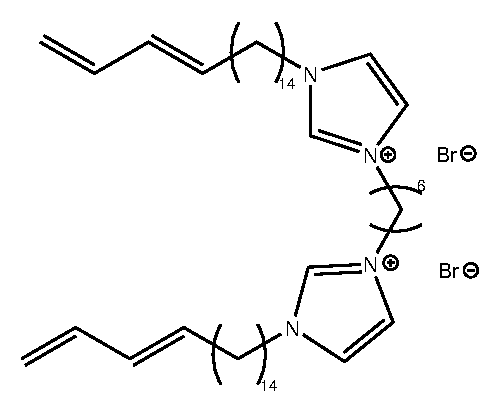
\includegraphics[trim=-2cm 0 0 0, clip, height=4.5cm]{Dibrpyr14.eps}
%        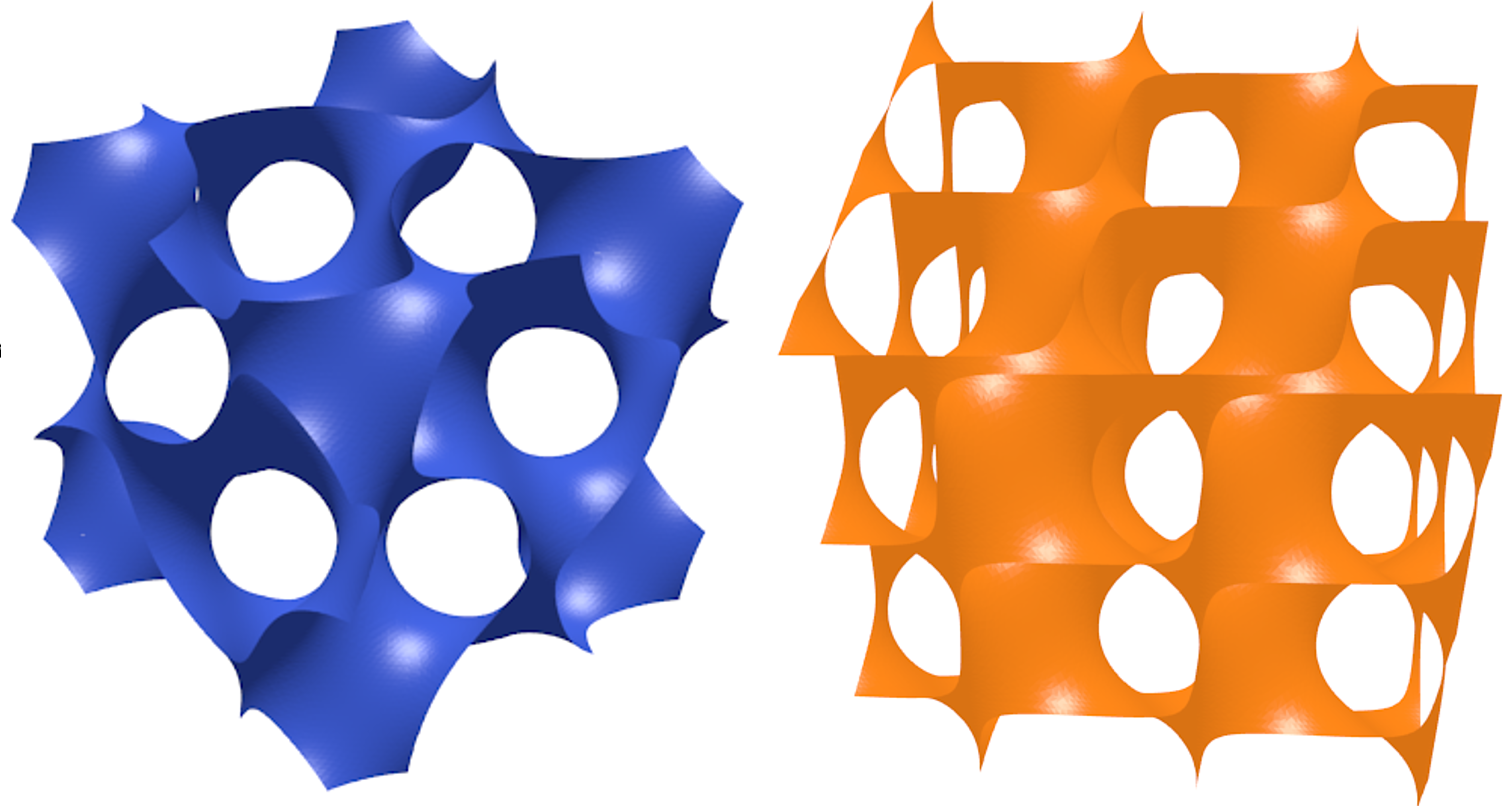
\includegraphics[height=4.5cm]{bcc_phases.png}
%        \caption{}\label{fig:bcc_phases}
%  \end{subfigure}
%  \hspace{1cm}
%  \begin{subfigure}{0.45\textwidth}
%        \centering
%        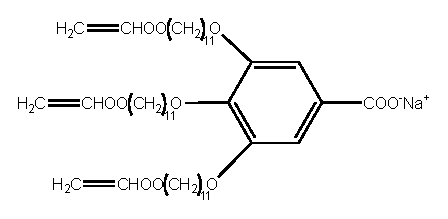
\includegraphics[trim=0 -0.5cm 0 -0.5cm, clip, height=4.5cm]{NaGA3C11.eps}
%        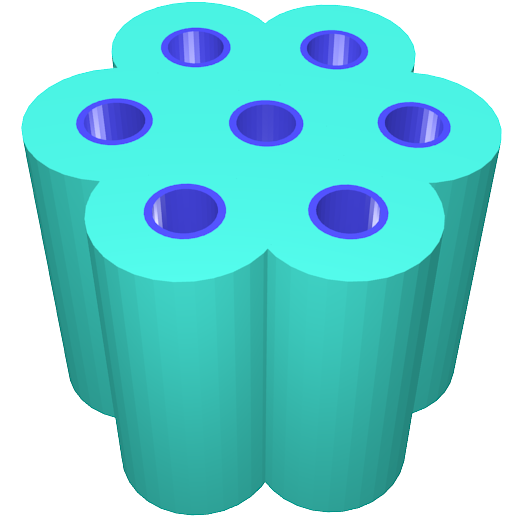
\includegraphics[height=4.5cm]{hexagonal_packing.png}
%        \caption{}\label{fig:hII_phase}
%  \end{subfigure}
%%MRS5: not sure Q should be in here.  Could cut length by removing some of the detail about Q phase, since it 
%%isn't discussed in the paper. 
%  \caption{The choice of LLC monomer and solvent leads to different accessible liquid
%        crystalline phases. The monomer shown in (a) forms the Q\textsubscript{I} phase
%        in either the Ia3d (left) or Pn3m (right) space group. The surfaces shown
%        represent the interface between the hydrophilic and hydrophobic regions of the unit
%        cell. 
%        %MRS7: not needed
%        %As pictured, we assume that each region occupies an equal volume. 
%        The
%        monomer shown in (b) will form the hexagonal columnar phase
%        (H\textsubscript{II} in the presence of water or Col\textsubscript{h} when no
%         water is present) The blue region represent the hydrophilic pores while the cyan region represents the surrounding hydrophobic monomer tails.}\label{fig:bcc_v_hII}
%  \end{figure}

  %Nanostructured porous membrane materials have become increasingly popular for
  %aqueous separations applications such as desalination and biorefinement because
  %they offer the ability to control pore architecture at the molecular scale,
  %thereby permitting the design of solute-specific separation membranes
  %\cite{humplik_nanostructured_2011}. One can achieve most membrane-based aqueous separations of
  %small molecules using reverse osmosis (RO) or nanofiltration
  %(NF) \cite{van_der_bruggen_review_2003}. While RO and NF have seen many
  %advances in the past few decades, they are far from perfect separation 

   %MRS4: these two paragraphs are perhaps not ideal.  They describe the process
  %of making the membranes, but that is not what we need as the introduction to
  %THIS paper.  Instead, you need to focus on the strength/issues with RO and
  %NF that motivate this research.
  % BJC2: The point I am trying to make is that the way the membranes are made 
  % results in either low selectivity or low permeability. I could just state
  % that, or give a little background on the processes to make the point more
  % tangible

  %Commercial RO membranes are typically dense thin-film composite (TFC)
  %membranes with a porous support layer and an active layer made of a polymer
  %matrix formed through interfacial polymerization \cite{jeong_interfacial_2007}.
  %During interfacial polymerization, a step-growth polymerization reaction occurs
  %at the interface of an aqueous monomer solution that has been soaked into the
  %support layer, and an organic solution of a second monomer. The polymer matrix
  %is dense and highly cross-linked which gives high rejections but low
  %permeability. 

  %During membrane fabrication,
  %aqueous diamine solution is allowed to penetrate into the polysulfone support
  %layer which is then immersed in trimesoyl chloride, a compound that is
  %immiscible in water. Diamine polymerizes with trimesoyl chloride at the
  %solution interface and creates a thin film that physically adheres to the
  %polysulfone support. 
 
%  solution.  Through the use of a non-solvent, a polymer-rich and polymer-poor
%  phase is formed. A membrane is created as the polymer-poor phase forms pores in
%  the polymer-rich phase. 
%  During phase inversion, a thin polymer film is precipitated out of a polymer

%  NF membranes are typically porous membranes made by a phase-inversion
%  process. The most widely used phase-inversion process is immersion
%  precipitation, during which one submerges a polymer, dissolved in a solvent, in
%  a non-solvent. A solid, porous polymer membrane is all that remains once all
%  solvent has been removed by non-solvent exchange
%  \cite{smolders_microstructures_1992}.  The resultant pores are polydisperse in
%  size, which hurts membrane selectivity. A second technique used to create NF
%  membranes is call track-etching in which a polymer film is bombarded with
%  charged particles, then chemically etched to create pores
%  \cite{apel_track_2001}. The pores are uniform, which benefits selectivity;
%  however, the membranes have a low porosity and subsequently low permeability. 
 
%MRS3: this is a little disconnected to the contents as well.  You want
%the paper to explain the why of doing this research.  Paragraph gives background, but doesn't motivate. 

%  Current commercial RO membranes are thin film composite membranes with a
%  porous support layer and an active layer made of a dense polymer matrix. The
%  membranes are unstructured with tortuous and polydisperse diffusion pathways.
%  Separation occurs based on differences in solubility and diffusivity of solutes
%  within the polymer matrix \cite{wijmans_solution-diffusion_1995}. With
%  optimization, one can exploit these differences to create a functional
%  selective barrier. RO operation costs are suboptimal because high feed
%  pressures are required in order to achieve a useful solvent flux. 

  %BJC : I don't know that this paragraph fits.  
  %MRS3: not really. Maybe take a look at Osuji's recent review (2016, I think) that addresses applications of nanostructured membranes and uses.  Could rewrite the introduction to be more about the general possibilities of nanostructured membranes, not just desalination.  It should be an introduction to what you will talk about in the paper, not to everything related.
 % Improved RO membranes can make desalination more sustainable. Only 0.5\% of
 % the world's water is fresh. Desalination is an important source of potable
 % water, necessary in order to keep up with demand generated by a rapidly growing
 % global population. Although RO is currently the cheapest form of desalination,
 % the cost must be further decreased in order to meet demand. A typical seawater
 % desalination process requires feed pressures in the range of 800 to 1000 psi
 % \cite{fritzmann_state---art_2007}. By designing better membranes for
 % desalination, we can achieve higher water fluxes and reduce feed pressure
 % requirements which will decrease the cost of fresh water production.
 % \cite{humplik_nanostructured_2011}.  

  % financially straining developing regions and contributing strongly to
  % CO\textsubscript{2} emissions. \cite{mcginnis_global_2008} Moreover,
  % designing RO membranes to achieve targeted separations of specific solutes
  % in a complex feed solution is nearly impossible

  %NF was introduced as an intermediate between RO and ultrafiltration, having
  %the ability to separate organic matter and salts on the order of one nanometer
  %in size. Explicit pore pathways running through the thickness of the membrane
  %permit high solvent fluxes at lower pressures than RO. NF membranes typically
  %have a surface charge resulting from ionizable groups which affords separation
  %of ions smaller than the pore radius by the mechanism of Donnan exclusion
  %\cite{van_der_bruggen_review_2003}. NF is often used as a precursor to reverse
  %osmosis since it can efficiently remove a significant portion of dissolved
  %solutes. Following NF pretreatment, RO can further purify the permeate. 
  %Unfortunately, NF membranes, like RO, possess a pore size
  %distribution which limits their ability to perform precise separations
  %\cite{bowen_modelling_2002}. 

%  The permeability-selectivity tradeoff has the potential to be overcome by
%  designing membranes at the molecular level. Next-generation nanoporous
%  membranes with high selectivity, permitted by a precisely controlled pore size,
%  and high permeability, allowed by its porous architecture, have the potential to
%  replace traditional RO and NF membrane technologies. 

%MRS3: I think that this paragraph probably should be couched in terms of what they COULD do, since are not widely used yet.
%MRS3: if talking about existing membranes, should cite performance.
%  Nanostructured membranes can bypass many of the performance issues which
%  plague traditional NF and RO membranes. One can accomplish targeted separations
%  with high selectivity by tuning shape, size and functionality of the molecular
%  building blocks which form these materials. As a result, solute rejecting pores
%  can have their sizes tuned uniformly, resulting in strict size cut-offs.
%  Entirely different mechanisms may govern transport in a given nanostructured
%  material which can inspire novel separation techniques.

%  Development of nanostructured porous materials has been limited by the
%  ability to synthesize and scale various fundamentally sound technologies.
%  Graphene sheets are atomically thick which results in excellent water
%  permeability but defects during manufacturing severely impact selectivity
%  \cite{cohen-tanugi_multilayer_2016}. Molecular dynamics (MD) simulations of
%  carbon nanotubes show promise \cite{humplik_nanostructured_2011}, but synthetic
%  techniques are unable to achieve scalable alignment and pore monodispersity
%  \cite{hata_water-assisted_2004,maruyama_growth_2005}. Zeolites have sub-nm
%  pores with a narrow pore size distribution, and MD simulations of these
%  materials show that they exhibit complete rejection of solvated ions
%  \cite{murad_molecular_1998}- however, experimental rejection was low and
%  attributed to interstitial defects formed during membrane synthesis
%  \cite{li_desalination_2004}. Consequently, there is a need for a scalable
%  nanostructured porous membrane. 

%  Polymeric membranes based on self-assembling lyotropic liquid crystals (LLCs)
%  are suitable candidates for aqueous separation applications. LLCs are
%  amphiphilic molecules that share the characteristic ability of nanostructured
%  porous membrane materials to create highly ordered nanostructures with the
%  added benefits of low cost and synthetic techniques feasible for large-scale
%  production \cite{feng_scalable_2014}. LLC systems created by the monomer
%  Na-GA3C11 (Fig.~\ref{fig:monomer}) have been extensively studied experimentally
%  \cite{feng_scalable_2014,smith_ordered_1997,zhou_supported_2005,resel_h2-phase_2000,feng_thin_2016}.
%  The neat Na-GA3C11 monomer forms the thermotropic liquid crystalline (TLC)
%  Col\textsubscript{h} phase (Fig.\ref{fig:assembly}). The presence of ca. 10
%  wt\% added water results in formation of the lyotropic H\textsubscript{II}
%  phase. In both cases, Na-GA3C11 monomers assembles into mesophases made of
%  hexagonally packed, uniform size, cylinders with hydrophilic head groups
%  oriented inward towards the cylinder center. This LLC assembly is then
%  polymerized in situ to form a cross-linked polymer network to stabilize the
%  structure. The hydrophilic region can act as a pore for aqueous separations
%  \cite{zhou_supported_2005}.  One can envision tailoring the pore region for
%  specific separations by changing the monomer chemistry
%  \cite{resel_h2-phase_2000}.

%  Research into the H\textsubscript{II} phase of polymerized LLC membranes has
%  been revived in recent years. 
%  During early stages of exploration, hexagonal
%  mesophases formed by Na-GA3C11 (Figure~\ref{fig:assembly}) could not be
%  macroscopically aligned, resulting in low flux membranes, and no clear route
%  towards scalable and economical filtration. 
%  For this reason, research efforts

  However, recently researchers have learned how to macroscopically align the
  hexagonal domains which has revived research into H\textsubscript{II} phase LLC
  membranes. In 2014, Feng et al.~showed that one can align Col\textsubscript{h}
  hexagonal domains, created by the monomer Na-GA3C11, using a magnetic field
  with subsequent cross-linking to lock the structure in
  place\cite{feng_scalable_2014}. In 2016, Feng et al. showed that one could
  obtain the same result by confining neat monomer between PDMS or glass
  substrates since hexagonal mesophases preferentially anchor perpendicular to
  both surfaces\cite{feng_thin_2016}.
%  the same result using a second technique termed soft confinement\cite{feng_thin_2016}.
  %MRS8: maybe say what it is, not just what it's named? 
  Current experimental efforts are focused on extending the method to the
  H\textsubscript{II} phase and characterizing the performance of these newly
  aligned systems.

  % BJC: Not sure this figure needs to be in the paper. 
  %MRS2: good question.  It helps give people context, which is necessary to
  %move forward.  Perhaps leave it in for now, though may need to get
  %permission to reprint it.
  %\begin{figure} \centering
  %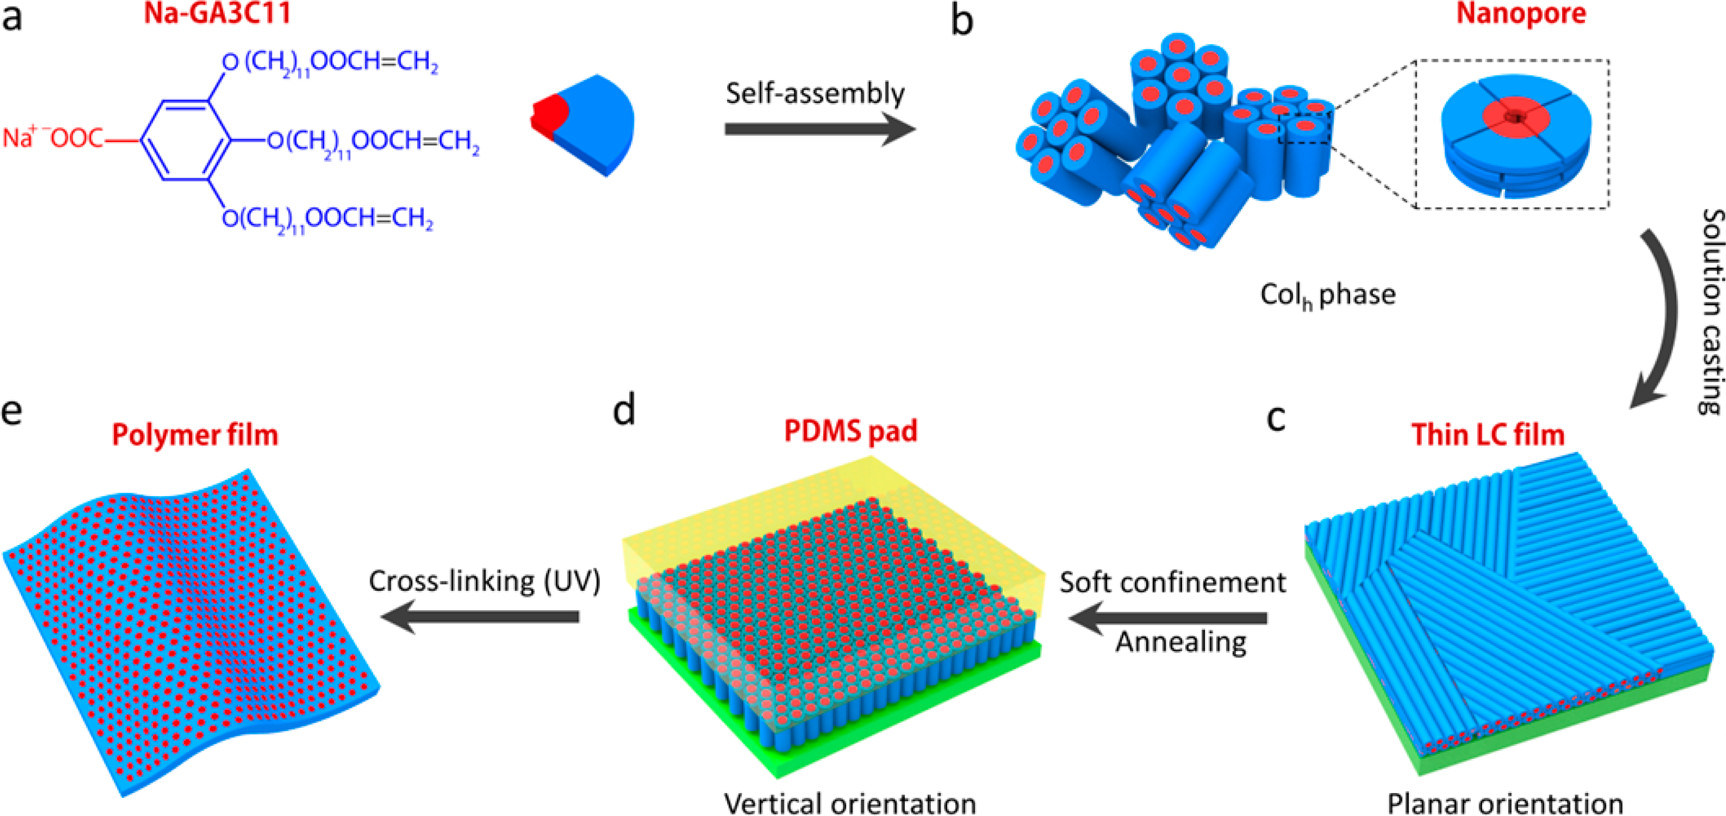
\includegraphics[width=\linewidth]{soft_confinement.png} \caption{The wedge
  %	  shaped liquid crystal monomer (a) self assembles into mesophases with
%		  hexagonally packed pores (b). The pores are made of stacked monomer disks. A
%		  sub-micron-thick film is created by casting a dilute solution of Na-GA3C11/THF
%		  solution onto a silicon substrate and and allowing the solvent to evaporate.
%		  The thin film contains nanoporous columns which lie parallel to the film plane.
%		  (d) When a soft PDMS pad is imposed to the thin film, with subsequent thermal
%		  annealing, the columns align perpendicular to the film plane. (e)
%		  Photo-cross-linking of the aligned film creates a mechanically stable thin film
%		  with vertically aligned nanopores}~\label{fig:soft} \end{figure}

  \begin{figure}
	\centering
	\begin{subfigure}{.3\textwidth}
		\centering
		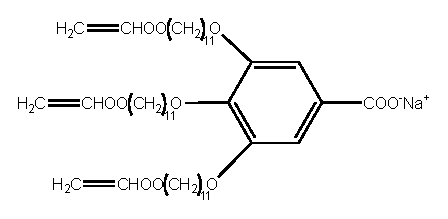
\includegraphics[width=\textwidth]{NaGA3C11.eps}
		\caption{}~\label{fig:monomer}
	\end{subfigure}
	\begin{subfigure}{.3\textwidth}
		\centering
		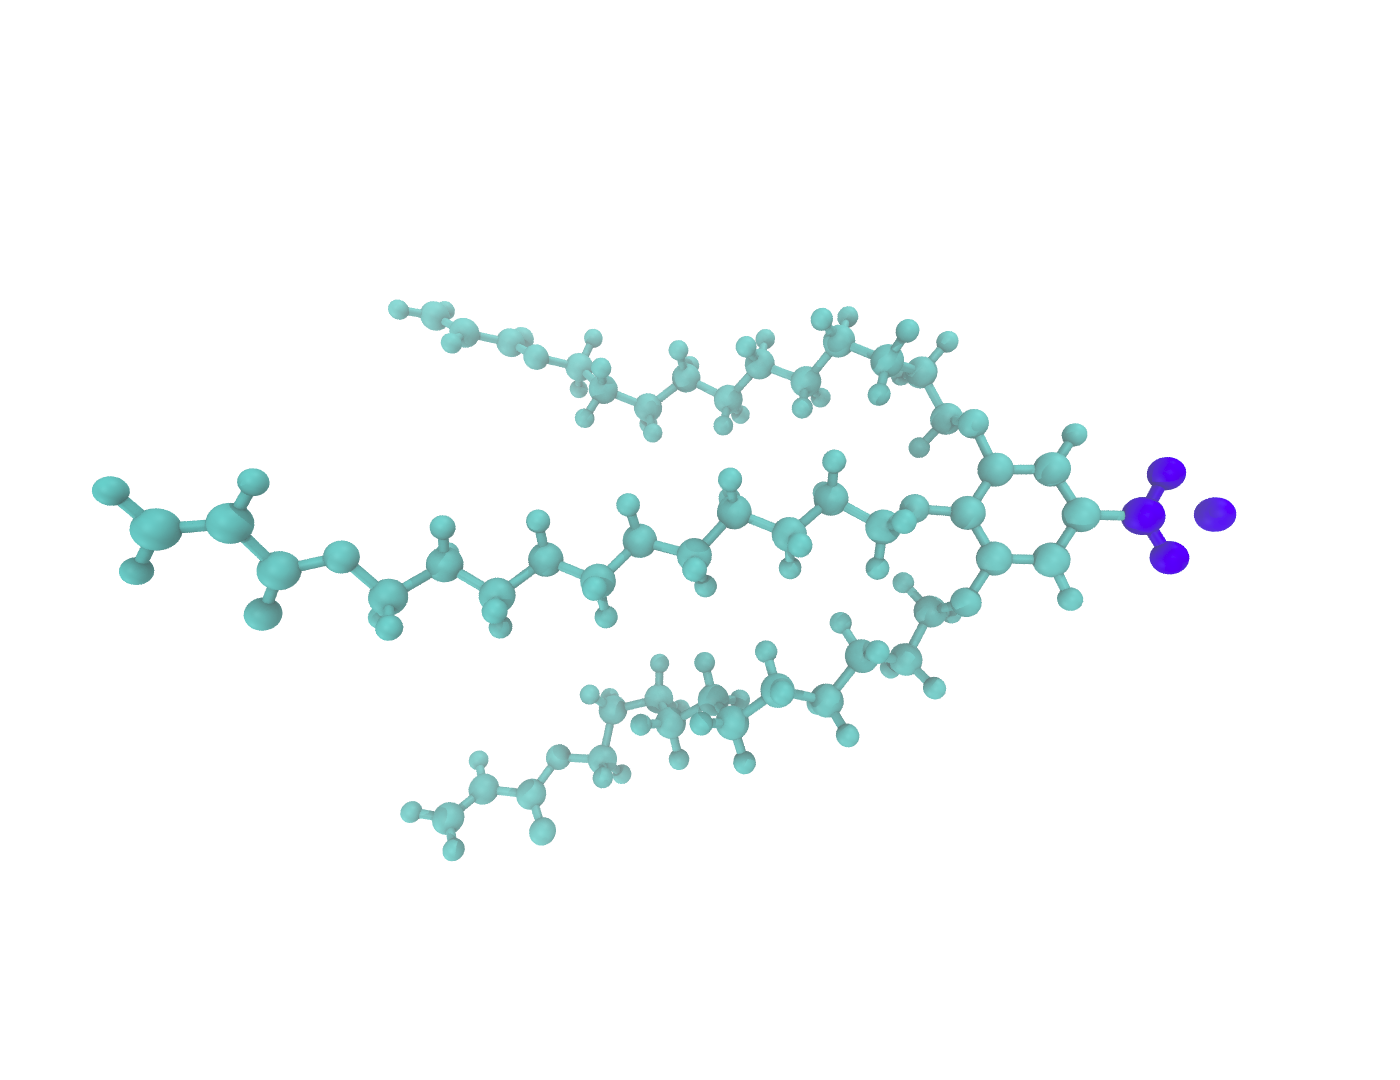
\includegraphics[width=\textwidth]{monomer_twocolor.png}
		\caption{}~\label{fig:atomistic_monomer}
	\end{subfigure}
	\begin{subfigure}{0.3\linewidth}
		\centering
		
\includegraphics[width=\textwidth]{wedge_thick.png}
		\caption{}~\label{fig:wedge}
	\end{subfigure}
		\begin{subfigure}{0.4\linewidth}
		\centering
		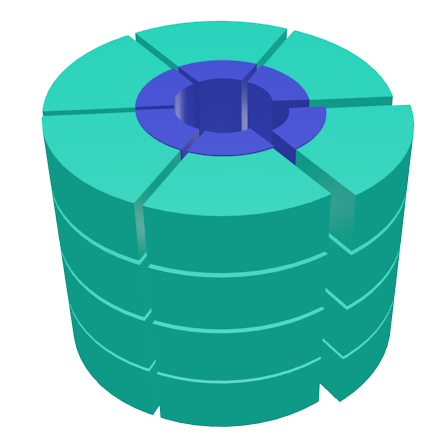
\includegraphics[width=\textwidth]{columns.png}
		\caption{}~\label{fig:wedge_layer}
	\end{subfigure}
	\begin{subfigure}{0.4\linewidth}
		\centering
		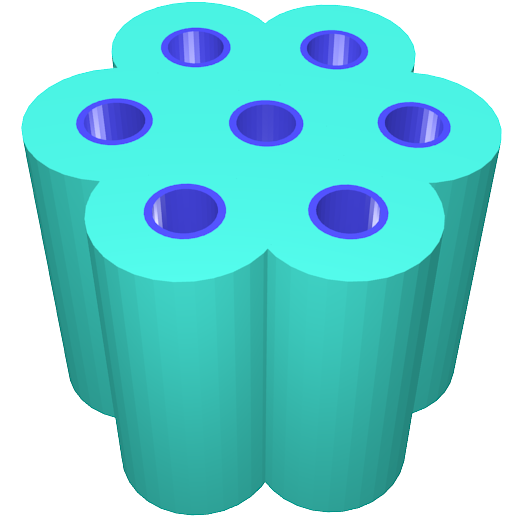
\includegraphics[width=\textwidth]{hexagonal_packing.png}
		\caption{}~\label{fig:hex_packing_simple}
	\end{subfigure}
	\caption{(a) The LLC monomer Na-GA3C11 (b) rendered atomistically (c)
	exhibits wedge-like character. (d) Monomers stack on top of each other with
	short range order and assemble into pores. (e) The hydrophilic head groups 
	(blue) facing towards the pore center. The pores assemble into hexagonally
	packed columnar mesophases.}~\label{fig:assembly}
  \end{figure}

  % BJC14: (5) justify need for simulations
  % BJC14: dishchinger example seems like a good thing to bring up since they 
  % explicitly state in the paper that they need a better understanding of
  % transport
  Our current understanding of the molecular details of LLC membranes'
  nanostructure is not sufficient to be able to precisely design them for
  specific separations. Dischinger et al. attempted to use an empirical model
  that correlates the physiochemical properties of the counterion used in a 
  Q\textsubscript{I} phase LLC membrane to solute rejection\cite{dischinger_effect_2017}.
  Although their model showed some qualitative agreement with experiment, the
  quality of fit of their model was limited due to complex solute-membrane 
  interactions which could not easily be modeled. Additionally, they observed
  an unexpected discrepancy in the relationship between uncharged solute
  rejection and water permeability which will require a more in-depth knowledge of
  the difference between solute and solvent transport.
  
  Over the past 20 years, H\textsubscript{II}-phase LLC
  polymer membrane studies have been limited primarily to Na-GA3C11 with some
  characterization done after minor structural modifications. Resel et al.~varied
  the length of the monomer tails and the counterion used and observed its effect
  on pore spacing \cite{resel_structural_2000}.  In a later study of rejection
  performance, it was shown that membranes formed by cross-linked Na-GA3C11 in
  the H\textsubscript{II} phase cannot separate solutes less than 1.2 nm in
  diameter because the pores are too large \cite{zhou_supported_2005}. We do not
  yet understand how to controllably reduce the effective pore size or how to
  tune the chemical environment in the nanopores of this or related materials for
  small molecule separations. The only source of predictive modeling for LLC
  systems have been macroscopic models that likely do not adequately describe
  transport at these length scales \cite{hatakeyama_water_2011}. Modeling with
  molecular detail could provide sufficient information about the mechanisms and
  chemical features to better inform experimental design of similar
  nanostructured membranes. 

  A molecular-level understanding of LLC membrane structure, enabled by
  molecular dynamics (MD) simulations, can provide guidelines to reduce the large
  chemical space available to design monomers for creation of separation-specific
  membranes. Useful molecular-level modeling should incorporate a detailed picture of the
  nanoscopic pore structure which is crucial to understanding the role of
  monomer structure in solute transport and membrane design. 
  Atomistic molecular dynamics simulations can provide the required level of detail
  (Figure \ref{fig:detail}), assuming the force fields are sufficiently accurate.
  With such an atomistic model, we can directly observe molecular-level solute
  transport and suggest governing mechanisms. We can observe how the choice of
  head group interacts with solutes of interest. We can interchange
  counterions which may influence both the pore size and the strength of the
  Donnan potential. 
  %which affects the degree to which the membrane can exclude
  %charged species at the membrane surface. 

  In this study, we achieve a  more realistic atomistic description of LLC
  membranes than, to our knowledge, has ever previously been created, and explore
  what new structural information can be gained and what structure hypotheses are
  supported by this model. We validate the results using as much experimental
  information as possible. We are most interested in reproducing the conclusions
  about structure drawn from small angle X-ray scattering (SAXS) and wide angle
  X-ray scattering (WAXS) experiments as well as in matching ionic conductivity
  measurements \cite{feng_thin_2016}.

  \begin{figure}[!htb]
  \centering
	\begin{subfigure}{0.45\linewidth}
		\centering
		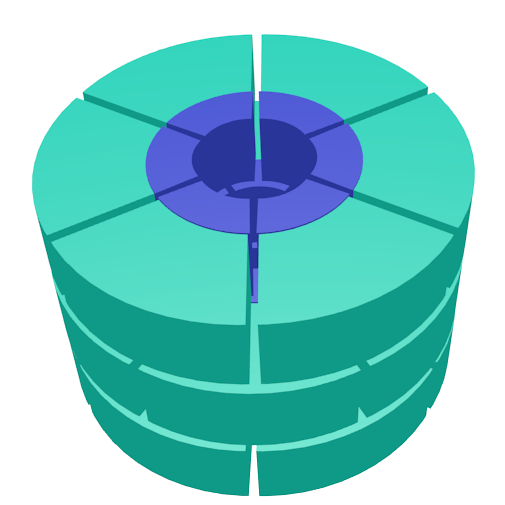
\includegraphics[width=\textwidth]{cartoon_pore.png}
		\caption{}~\label{fig:undetailed_pore}
	\end{subfigure}
	\begin{subfigure}{0.45\linewidth}
		\centering
		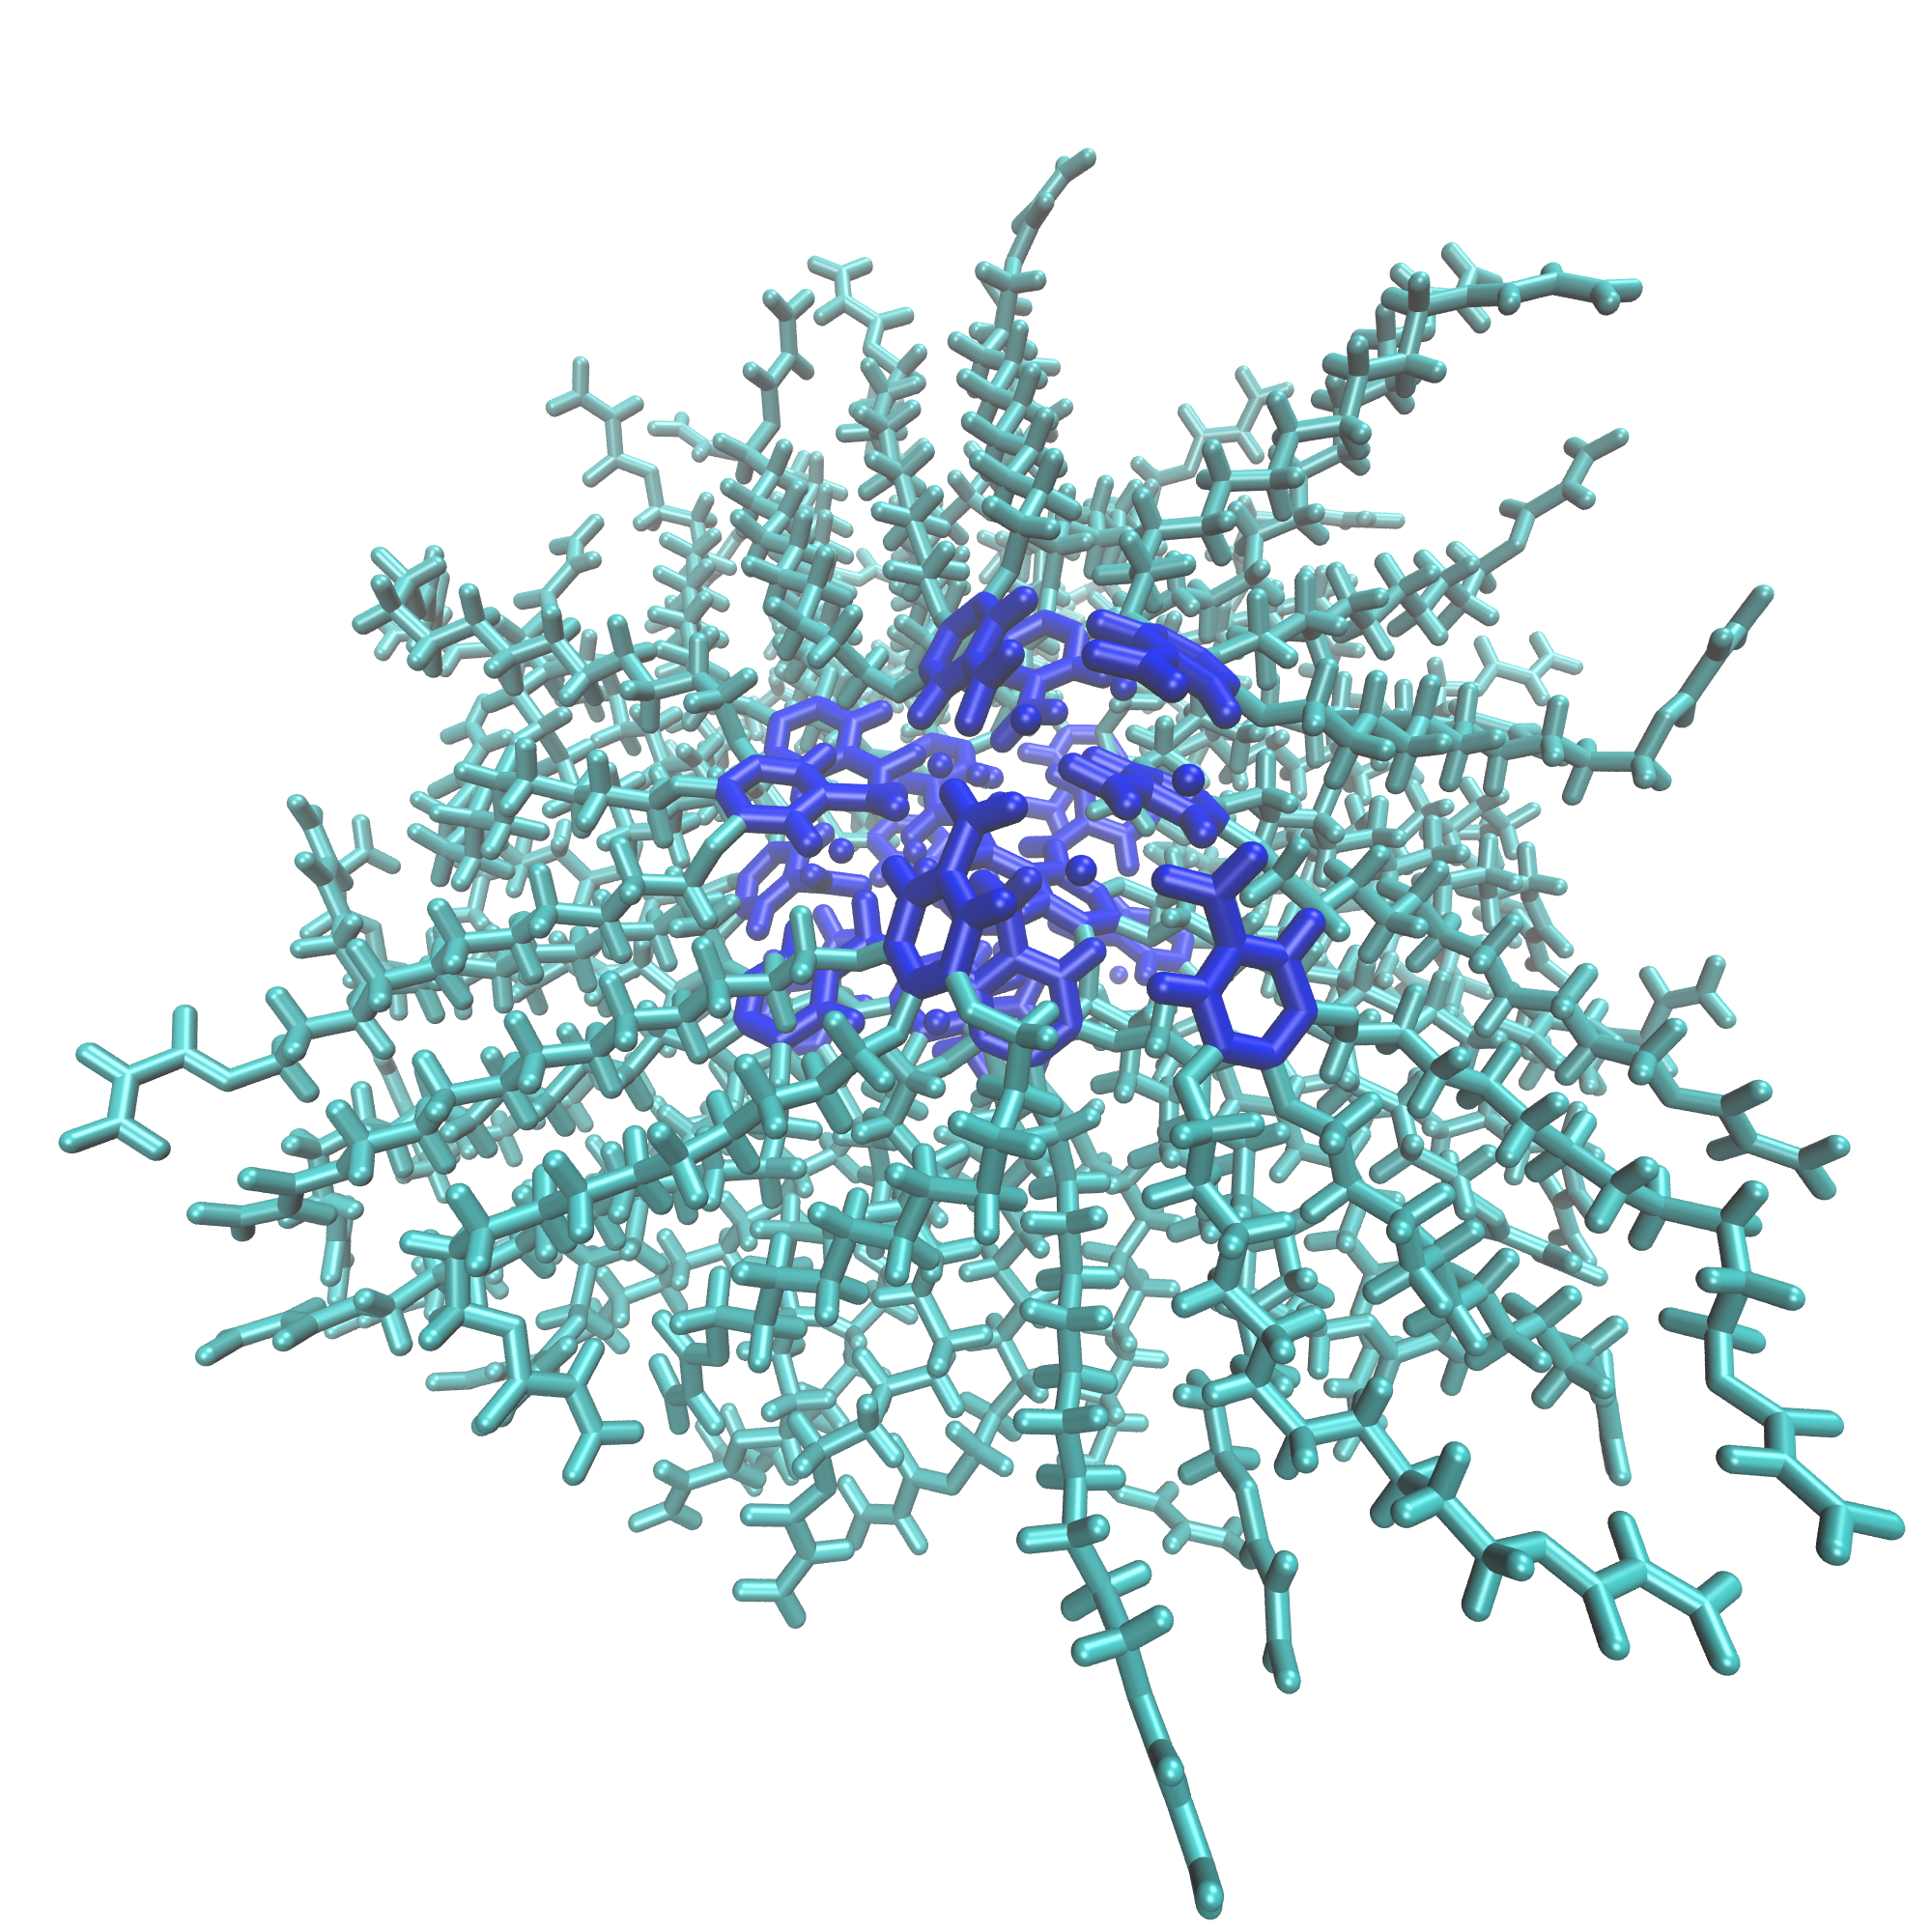
\includegraphics[width=\textwidth]{detailed_pore.png}
		\caption{}~\label{fig:detailed_pore}
	\end{subfigure}
    \caption{(a) Previous understanding of the pores are essentially speculations 
    based on limited chemical and experimental data. (b) We use detailed molecular 
    modeling in this paper in order to appropriately model the pore's complex architecture
    which is crucial to understanding the mechanism of solute transport. In both 
    pictures, the head group region is colored blue and the tail region is colored cyan.}~\label{fig:detail}
  \end{figure}
 
  In this paper, we perform molecular modeling of the Col\textsubscript{h}
  assembly formed by Na-GA3C11. Compared to the H\textsubscript{II} phase, the
  Col\textsubscript{h} phase is a simpler starting point. The system is not
  assembled in aqueous phase which allowed us to simulate longer timescales, and
  there exists detailed experimental characterization of the fully aligned state,
  including 2D wide-angle X-ray scattering (WAXS) patterns
  (Figure~\ref{fig:WAXS}) which are useful for reconstructing structural data. 
  
  %MRS8: I started tweaking the below, but it might be better just to eliminate.
  % Modeling of Col\textsubscript{h} will help in modeling 
  %H\textsubscript{II} in the future.
  %The two phases appear to share similar structural characteristics since the
  %pore spacings in each system are in close agreement
  %\cite{feng_thin_2016,resel_structural_2000}.
  
%  We used experimental small-angle X-ray scattering (SAXS) data from
%  \cite{feng_thin_2016} (Fig.~\ref{fig:SAXS}) and wide angle X-ray scattering
%  (WAXS) data (Fig.~\ref{fig:WAXS}, produced as described in
%  \cite{feng_scalable_2014}) for comparison to our model. We rely primarily on the 2D WAXS data
%  since it encodes all structural details down to the sub-nm scale.  
  There are five major features of interest present in the 2D experimental
  pattern shown in Figure~\ref{fig:WAXS}.

  \begin{enumerate} 
  
	\item \textit{R-$\pi$}: The location of the first is at $q_z$ = 1.7
	\AA$^{-1}$, corresponding to a real space separation of 3.7 {\AA}. Previous
	work~\cite{feng_scalable_2014} attributes this reflection to $\pi$-$\pi$
	stacking between aromatic rings in the direction perpendicular to the membrane
	plane, or z-axis \cite{feng_scalable_2014}. For simplicity, we will refer to
	this reflection as R-$\pi$.
 
	\item \textit{R-double}: A weak intensity line, located at exactly half
	the $q_z$ value of R-$\pi$ ($q_z$ = 0.85 \AA$^{-1}$), corresponds to real
	space periodicity of 7.4 \AA. Since this reflection corresponds to double
	the spacing of R-$\pi$ in real space, we will refer to it as R-double. 
	R-double has been previously interpreted as 2\textsubscript{1} helical ordering of aromatic
	rings along the $z$ axis\cite{feng_scalable_2014}.
        %meaning if one traces the 
	%positions of the aromatic rings with a helical curve, then for each full turn 
	%in the helix, one will encounter two aromatic rings.

	\item \textit{R-alkanes}: A low intensity ring located at $|\mathbf{q}|$ = 1.4
	\AA$^{-1}$ marks the third major reflection of interest. The real space
	separation corresponds to 4.5 \AA~ which is characteristic of the average
	spacing between packed alkane chains \cite{mcintosh_organization_1980}. We will
	call this reflection R-alkanes.

	\item \textit{R-spots}: Within R-alkanes, are four spots of higher
	relative intensity.  Accordingly, we name these reflections R-spots. The
	location of all spots is $\sim\,37^{\circ}$ from the $q_z$ axis in their
	respective quadrants. In many liquid crystal systems one can explain the spots
	as the product of alkane chains tilted with respect to the membrane
	plane\cite{govind_simple_2001}.
 
	\item \textit{R-pores}: The final feature corresponds to the spacing
	and symmetry of the pore columns. 
        %d\textsubscript{100} plane. This plane is geometrically
        %related the distance between pores.
	The feature, which we named R-pores, is characterized by reflections along the
	equatorial axis defined by $q_z$ = 0. The spacing between dots is indicative of
	the hexagonal symmetry of the packed pores. We observe the same information
	with higher resolution using SAXS (Fig.~\ref{fig:SAXS}). 

  \end{enumerate}

  \begin{figure}[!htb]
        \centering
                \begin{subfigure}[t]{0.495\linewidth}
                \centering
                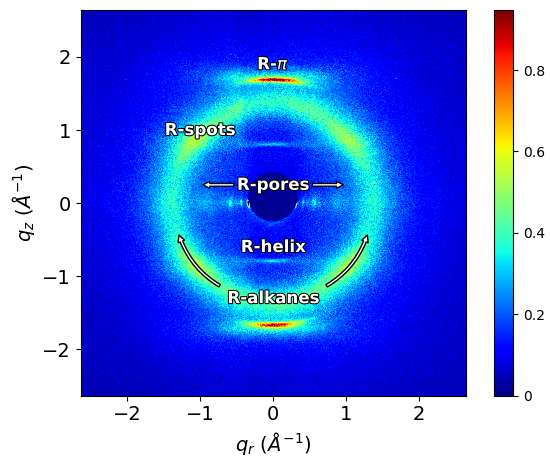
\includegraphics[width=\linewidth]{WAXS_annotated_words.png} 
                \caption{}\label{fig:WAXS}
        \end{subfigure}
	\begin{subfigure}[t]{0.405\linewidth}
                \centering
                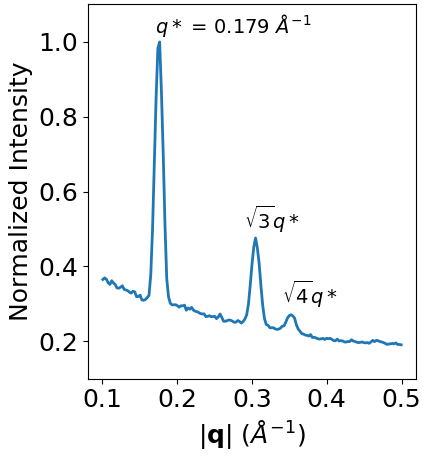
\includegraphics[width=\linewidth]{SAXS.png}
                \caption{}\label{fig:SAXS}
        \end{subfigure}
	\caption{(a) 2D WAXS gives details about repeating features on the
		order of angstroms. Experimentalists have explained each of the 5 major
		reflections present as follows: (R-$\pi$) Aromatic head groups $\pi-\pi$ stack
		3.7 \AA~apart. (R-double) Monomers arrange vertically in a 2\textsubscript{1}
		helix. (R-alkanes) Alkane chain tails pack 4.5 \AA~apart. (R-spots) Monomer
		tails are tilted with respect to the membrane plane. (R-pores) As derived from
		SAXS, the pores are spaced 4.12 nm apart and pack hexagonally (b) (Reproduced
		from \citenum{feng_thin_2016}) The repeat spacing in the 1D small angle X-ray
		scattering pattern is characteristic of hexagonal packing. The leading peak,
		q*, represents the distance between the d\textsubscript{100} planes. Using this
		distance, we know that the distance between pore centers is 4.12 nm.} 
	\label{fig:SWAXS}
 \end{figure}
  
 Despite having structural data, there is still information which experiment
 cannot definitively answer. Specifically, we want to know:
 \begin{enumerate}
    \item What is the density of monomers that pack around each hydrophilic core? 
    \label{point:monomernum}

 	Authors often describe this and similar systems as being made up of layers. A simple
 	molecular simulation study of a similar molecule suggested that there are 4 monomers
 	in each layer. Their estimation is based on a simulated system containing only 16 total
 	monomers which likely does not sufficiently model the chemical environment present in
 	the real system.~\cite{zhu_methacrylated_2006}. A separate calculation based on the 
 	volume of the liquid crystal monomers proposes that there are seven monomers in each 
 	layer~\cite{resel_structural_2000}. 

  	We are careful to avoid the term 'layers' since many liquid crystalline systems
 	have long range order in 1 or 2 spatial dimensions and short range order in 	
 	the other dimensions.~\cite{chaikin_principles_1995}  % page 58
 	In the system we are studying, there are long-range 2D correlations in the 
 	hexagonal array of pores (xy plane) and short range z-direction correlations between 
        stacked columns of monomers. In this study, we use atomistic molecular modeling
        to study how the system's structure is affected by the density of these monomer columns
        that surround each pore's hydrophilic core. 

	\item What structural motif best matches experimental 2D WAXS patterns?\label{point:xrdmatch}

	On the short timescales accessible to MD (even the 100's of nanoseconds of simulation 
	performed here are short compared to experimental timescales), we observe distinct metastable
	configurations which depend on starting configuration. We simulated XRD patterns of our system and 
	compared them to experimental 2D WAXS patterns (Figure~\ref{fig:WAXS}) so that we ensure our
	model creates a nanoscopic chemical environment maximally consistent with experiment within 
	the constraints	of our forcefield. Using this approach, we are able to confirm some previous
	interpretations	of the WAXS pattern and refute others. 
	
	%BJC5: I could add brief references to other LLC studies which look at hexagonal phase, but
	% without scrutinizing the structural details. In other words, other authors have gotten 
	% hexagonal phases with self-assembly, but they can't prove that their structure is the same
	% as experiment. The best there are, are 1D structure factors in the small angle regime.

        \item Is it necessary to include any water in order to appropriately model the 
        Col\textsubscript{h} phase? \label{point:water}

	While the Col\textsubscript{h} phase is described as dry, it is likely
	that small amounts of ambient water are absorbed into the system. The hydrogen
	bonding network formed by the water may play a role in structuring the pore. We
	used simulated X-ray diffraction (XRD) patterns to uncover any 
        %see if there is any
	meaningful structural difference between a "dry" and a "wet" system.

	\item What is the detailed atomistic structure of the pores?\label{point:composition}

	The limited picture that experiment provides tells us that there are hexagonally packed, 
	hydrophilic regions where transport is likely to occur. One may instinctively imagine these 
	regions as tube-like pathways with well-defined boundaries. We explored the composition
	of the pores, the partition between the hydrophilic and hydrophobic regions, and its 
	sensitivity to initial configuration, including both dry and wet systems. 

  \end{enumerate}
  
%  In order to appropriately model transport in these ordered, nanoporous
%  organic systems, we must first gain a thorough understanding of the nanoscopic
%  structure of LLC polymer membranes. Our current level of understanding about
%  the structure at the nanoscale is limited. Using X-ray diffraction and TEM data
%  we can infer that monomers aggregate into hexagonally packed columns with their
%  head groups facing towards the column center. There remain several key questions
%  that we will investigate in order to expand this understanding: 
%
%  \begin{enumerate}

%BJC3: reworded a lot of these to be more in line with Matt's way of thinking about LC systems
%MRS6: formatting suggestion
%  \item \textit{If layers do exist, how many monomers constitute a single layer? \label{point:monomernum}} 
%  \item \textit{How many monomers pack around a single pore column?\label{point:monomernum}} 
%  A simple molecular simulation study of a similar molecule suggested that
%  4 monomers radially pack around hydrophilic pore columns \cite{zhu_methacrylated_2006}.
%  Their model likely does not sufficiently imitate the chemical environment present
%  in the real system since it only contains 16 total monomers. A separate calculation
%  for NA-GA3C11, based on the estimated volume of the liquid crystal monomers,
%  proposes that each pore is surrounded by seven
%  monomers\cite{resel_structural_2000}. Our best chance to answer this question
%  is by using a molecular model orders of magnitude larger than any other
%  reported atomistic liquid crystal membrane simulation, as we present here. We
%  will directly change the density of monomers in each pore and note its effect
%  on membrane structure.
%
%%  \item \textit{How do monomers in each layer position themselves with respect to
%%  surrounding layers? \label{point:orientation}}
%  \item \textit{In what orientation do monomer head groups stack on top of each
%  other \label{point:orientation} 
%  $\pi$-$\pi$ stacking interactions between aromatic monomer head groups may be
%  a driving force of self-assembly in this system \cite{gazit_possible_2002}. Gas
%  phase \textit{ab initio} studies of benzene dimers have shown a clear energetic
%  advantage for parallel displaced and T-shaped $\pi$-$\pi$ stacking
%  conformations over a sandwiched conformation \cite{sinnokrot_estimates_2002}.
%  Substituted benzene rings exhibit an even stronger $\pi$-$\pi$ stacking
%  attraction which favors the parallel displaced configuration in all cases except
%  where the substitutions are extremely electron withdrawing  
%  \cite{waller_hybrid_2006,ringer_effect_2006}. We did not consider the T-shaped 
%  configuration due to its geometric incompatibility with a hexagonal columnar phase.
%  The entropic contribution of the long alkane tails should overwhelm any attraction
%  between aromatic head groups in the T orientation. We limit our studies to
%  comparison of systems built in the parallel displaced and sandwiched configurations.  

% BJC3: I don't want to limit X-ray diffraction patterns just to deciding between
% parallel displaced and sandwiched. Since it doesn't actually decide either way.  
%  In this study, we
%  compare simulated X-ray diffraction patterns to experiment in order to deduce
%  which stacking configuration is most likely. We also dive deeper into the
%  origin of features present in the 2D diffraction patterns.  

%  \item \textit{Does our model support the existence of layers and if so, how well
%  defined are the layers? \label{point:layers}}
%  Indications of strong $\pi$-$\pi$ stacking interactions in the direction
%  perpendicular to the membrane plane, combined with the wedge-like character of
%  the LLC monomers, suggests that monomers should arrange into disks that stack in
%  layers. $\pi$-$\pi$ stacking will only occur between the aromatic
%  monomer head groups which leaves no description of what is happening in the
%  monomer tail region. The tails may entangle isotropically while maintaining
%  stacking order among headgroups.  
% BJC3:rephrasing everything about the above question. 
%  \item \textit{How strong are stacking correlations between monomer head groups?
%  \label{point:layers}}
  

%BJC3: Going to talk about temperature rather than ordered/disordered states
%  \item \textit{Can the system exist in other metastable states or phases that are not
%  accessed during experiments? \label{point:metastable}}
%  There remains the possibility that there is more than one metastable state
%  associated with a given LLC phase. Simulating a membrane atomistically
%  requires many atoms which limits the timescales acessible with MD. It is
%  reasonable to expect that we will generate configurations which are kinetically
%  trapped in a metastable free energy basin. We must be able to identify which
%  states 
  %MRS6: best not to set up too high expectations
  %is produced experimentally.
%  are most consistent with experiment.

%  \item \textit{What constitutes a pore, and what are the details of its composition?
%  \label{point:poredefinition}}
%  The limited picture that experiment provides tells us that there are
%  hexagonally packed, hydrophilic regions where transport is likely to occur.
%  One may instinctively assume that these regions are hollow tube-like pathways.
%  We will explore the composition of the pores and the partition between the
%  hydrophilic and hydrophobic regions. 
% 
%
%  \item \textit{Is it necessary to include any water in order to appropriately model
%  the Col\textsubscript{h} phase? \label{point:water}}
%  While past work describes the Col\textsubscript{h} phase as dry~\cite{feng_scalable_2014}, 
%  it has been suggested by experimentalists, in
%  unpublished communications, that it is likely that neat monomer leaches small
%  amounts of ambient water. Experimentally, achieving a hexagonal phase with a
%  completely dry system has proven difficult. If neat monomer sits in ambient
%  conditions, its color turns from transparent to slightly opaque and a hexagonal
%  phase forms. Although we will not explore whether water is necessary for
%  self-assembly, we hypothesize that the hydrogen bonding network formed by the
%  water may play a role in structuring the pores and holding together the
%  hexagonal phase. We can look at correlation functions and use simulated X-ray
%  diffraction patterns to see if there is any meaningful structural difference
%  between a ``dry'' and ``wet'' system.
%
%  \end{enumerate}
  
  %Once we have addressed all of the above questions, we must show that the 
  %developed molecular model is consistent with physical observations so that we
  %can rely on conclusions drawn about structural features characteristic of 
  %the system.

  \section{Methods}
 
  \subsection{Monomer Parameterization}

  We parameterized the liquid crystal monomer Na-GA3C11 using the Generalized AMBER
  Force Field (GAFF) \cite{wang_development_2004} with the Antechamber package
  \cite{wang_automatic_2006} provided with AmberTools16
  \cite{case_ambertools16_2016}. We assigned atomic charges using the am1bccsym
  method of \texttt{molcharge} shipped with QUACPAC from Openeye Scientific
  Software. We ran all molecular dynamics simulations using GROMACS 2016
  \cite{bekker_gromacs:_1993,berendsen_gromacs:_1995,van_der_spoel_gromacs:_2005,hess_gromacs_2008}.

  We generated an ensemble of characteristic, low-energy vacuum monomer
  configurations by applying a simulated annealing process to a
  parameterized monomer. We cooled monomers from 1000K to 50K over 10
  nanoseconds. We randomly pulled a low energy configuration from the
  trajectory then reassigned charges using \texttt{molcharge}. Using the new
  charges, we annealed the monomer system again and pulled a random monomer
  configuration from the trajectory which we used for full system
  construction (Figure~\ref{fig:build_procedure}a). See section S-\ref{S-section:parameterization} 
  for further detail of the parameterization process.

  \subsection{Unit Cell Preparation}

  The timescale for self-assembly of monomers into the hexagonal phase is
  unknown and likely outside of a reasonable length for an atomistic simulation,
  calling for a more efficient way to build the system. Previous work has shown
  a coarse-grained model self assemble into the H\textsubscript{II} phase
  configuration in $\sim$1000 ns \cite{mondal_self-assembly_2013}.  We
  attempted atomistic self-assembly by packing monomers into a box using Packmol
  \cite{martinez_packmol:_2009}. Simulations of greater than 100 ns show no
  indicators of progress towards an ordered system (see section S-\ref{S-section:self_assembly}). 
  To bypass the slow self-assembly process, we use Python scripts to assemble monomers
  into a structure close to one of a number of hypothesized equilibrium configurations
  (Figure~\ref{fig:build_procedure}).
  %MRS13: Would be nice to say we put the scripts on GitHub.  Additional details about which scripts can be in supporting.
  These initial structures may result in equilibration into slowly-intercoverting metastable states, an issue we will address later in the paper. 
  % BJC5: This needs to be modified to reflect columnar build procedure
  \begin{figure}[!htb]
  \centering
  \begin{subfigure}[t]{0.45\textwidth}
  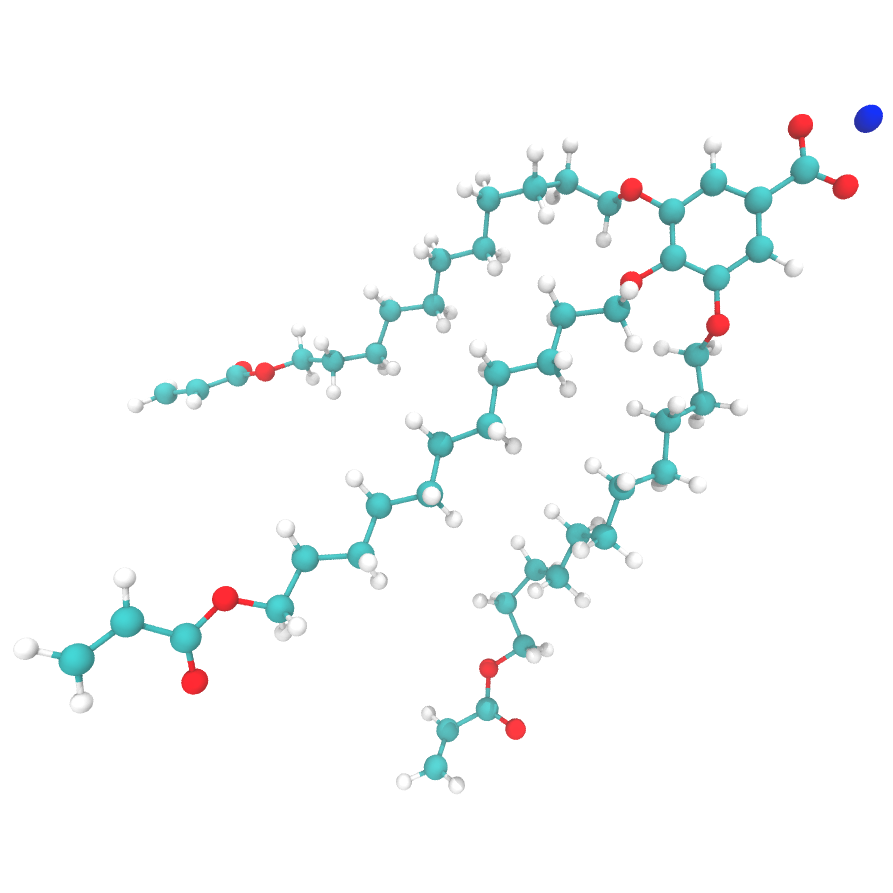
\includegraphics[width=\linewidth]{monomer_diagonal.png}
  \caption{}
  \end{subfigure}
  \begin{subfigure}[t]{0.42\textwidth}
  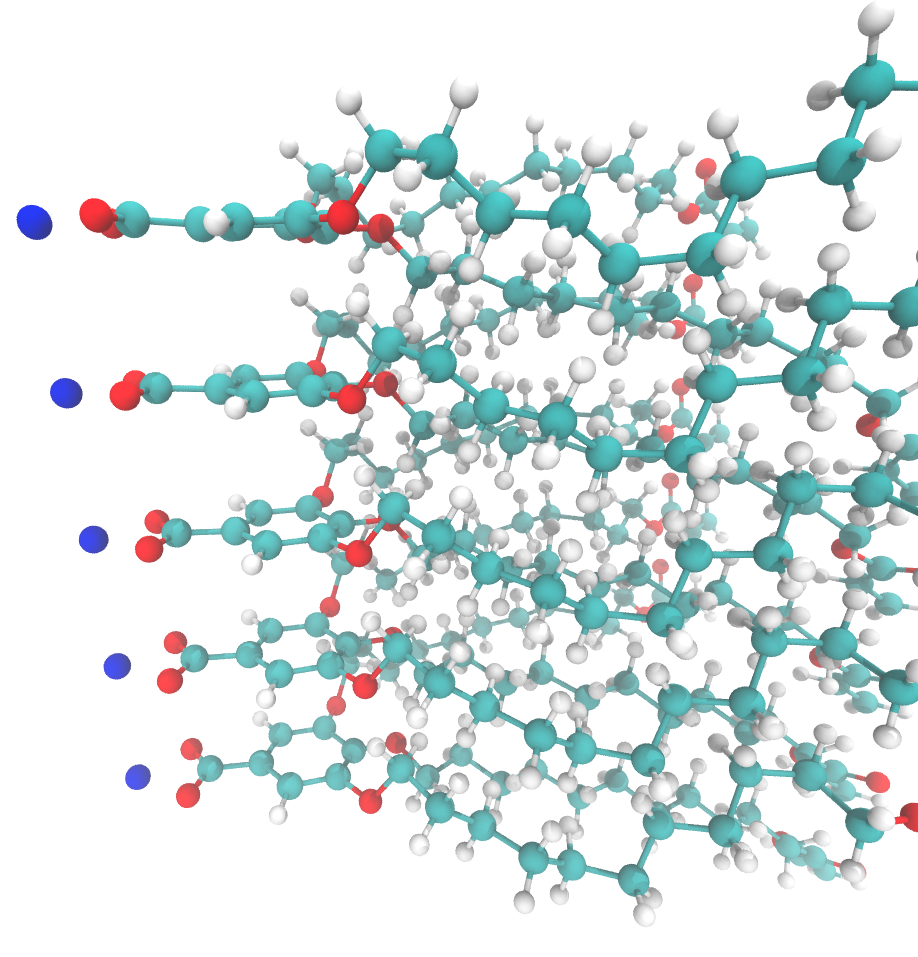
\includegraphics[width=\linewidth]{stacked_monomers.png}
  \caption{}
  \end{subfigure}
  \begin{subfigure}[t]{0.35\textwidth}
  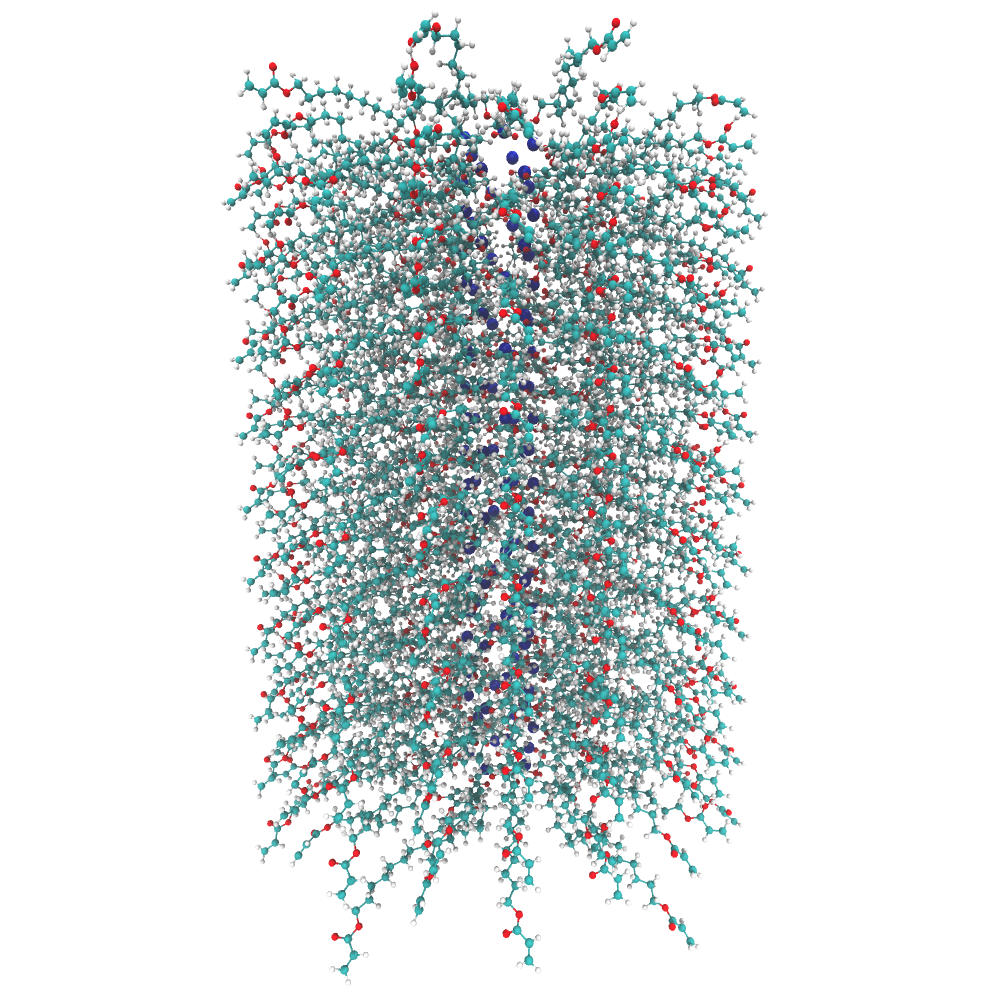
\includegraphics[width=\linewidth]{initial_pore.png}
  \caption{}
  \end{subfigure}
  \begin{subfigure}[t]{0.45\textwidth}
  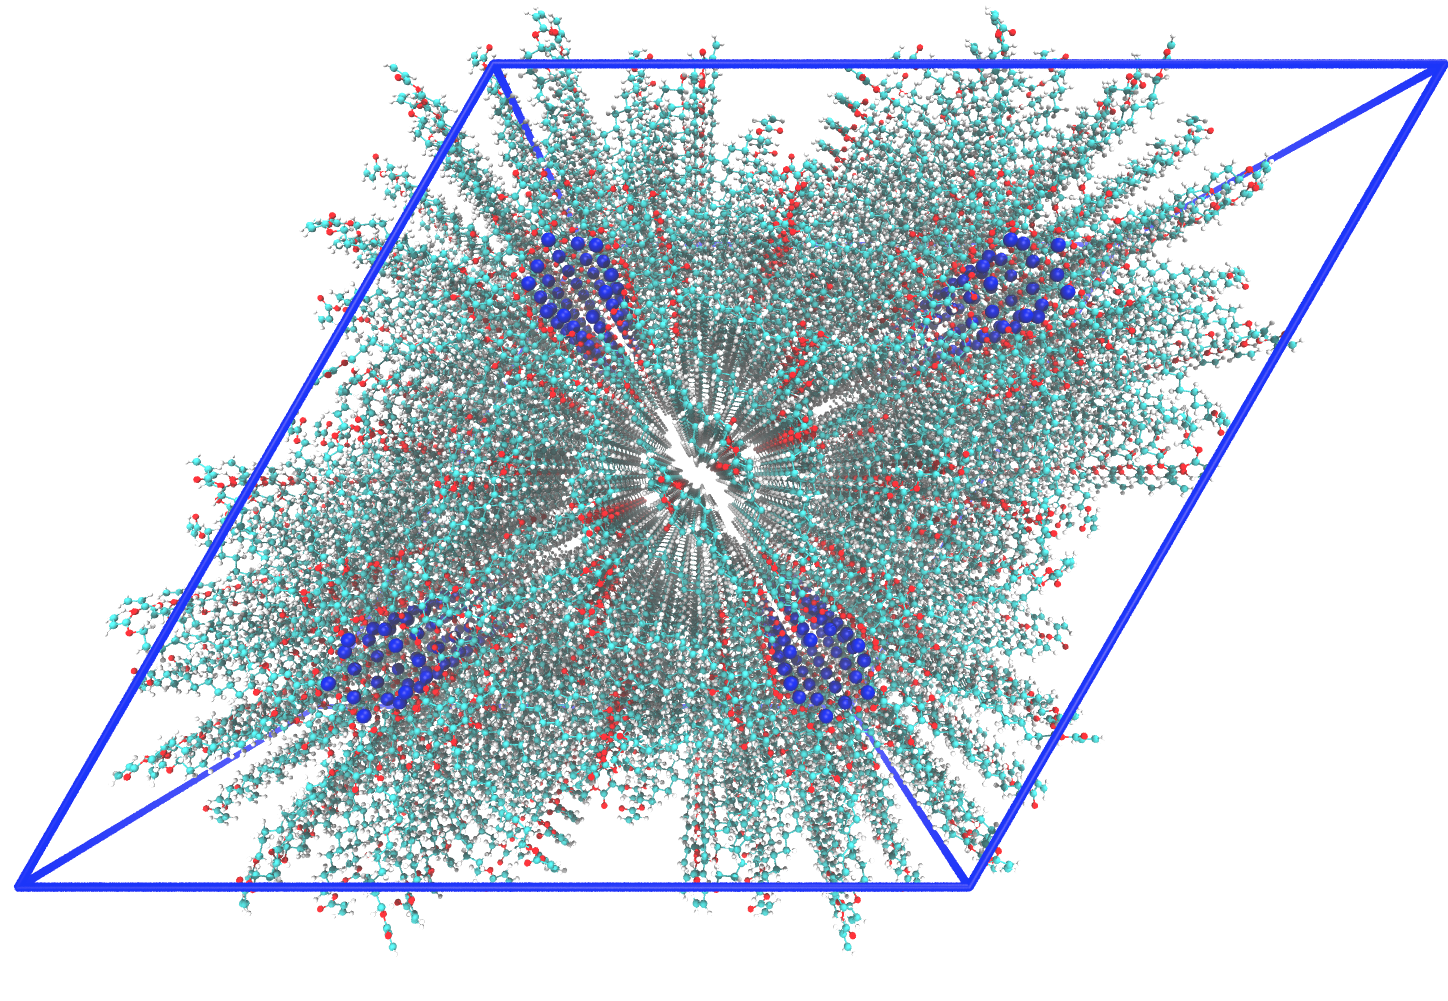
\includegraphics[width=\linewidth]{initial_unit_cell.png}
  \caption{}
  \end{subfigure}
  \caption{(a) We parameterized a single monomer and annealed it to produce a low energy
		configuration. (b) We assembled monomers into columns by stacking them on top of each 
		other. (c) We duplicated each column and rotated them to create hydrophilic pore centers.
		We chose to stack twenty monomers into each column. (d) We duplicated the pores and 
		placed them into a monoclinic unit cell with hexagonal symmetry.}\label{fig:build_procedure}
  \end{figure}
  
  %BJC7: old
%  \begin{figure}
%	\centering
%	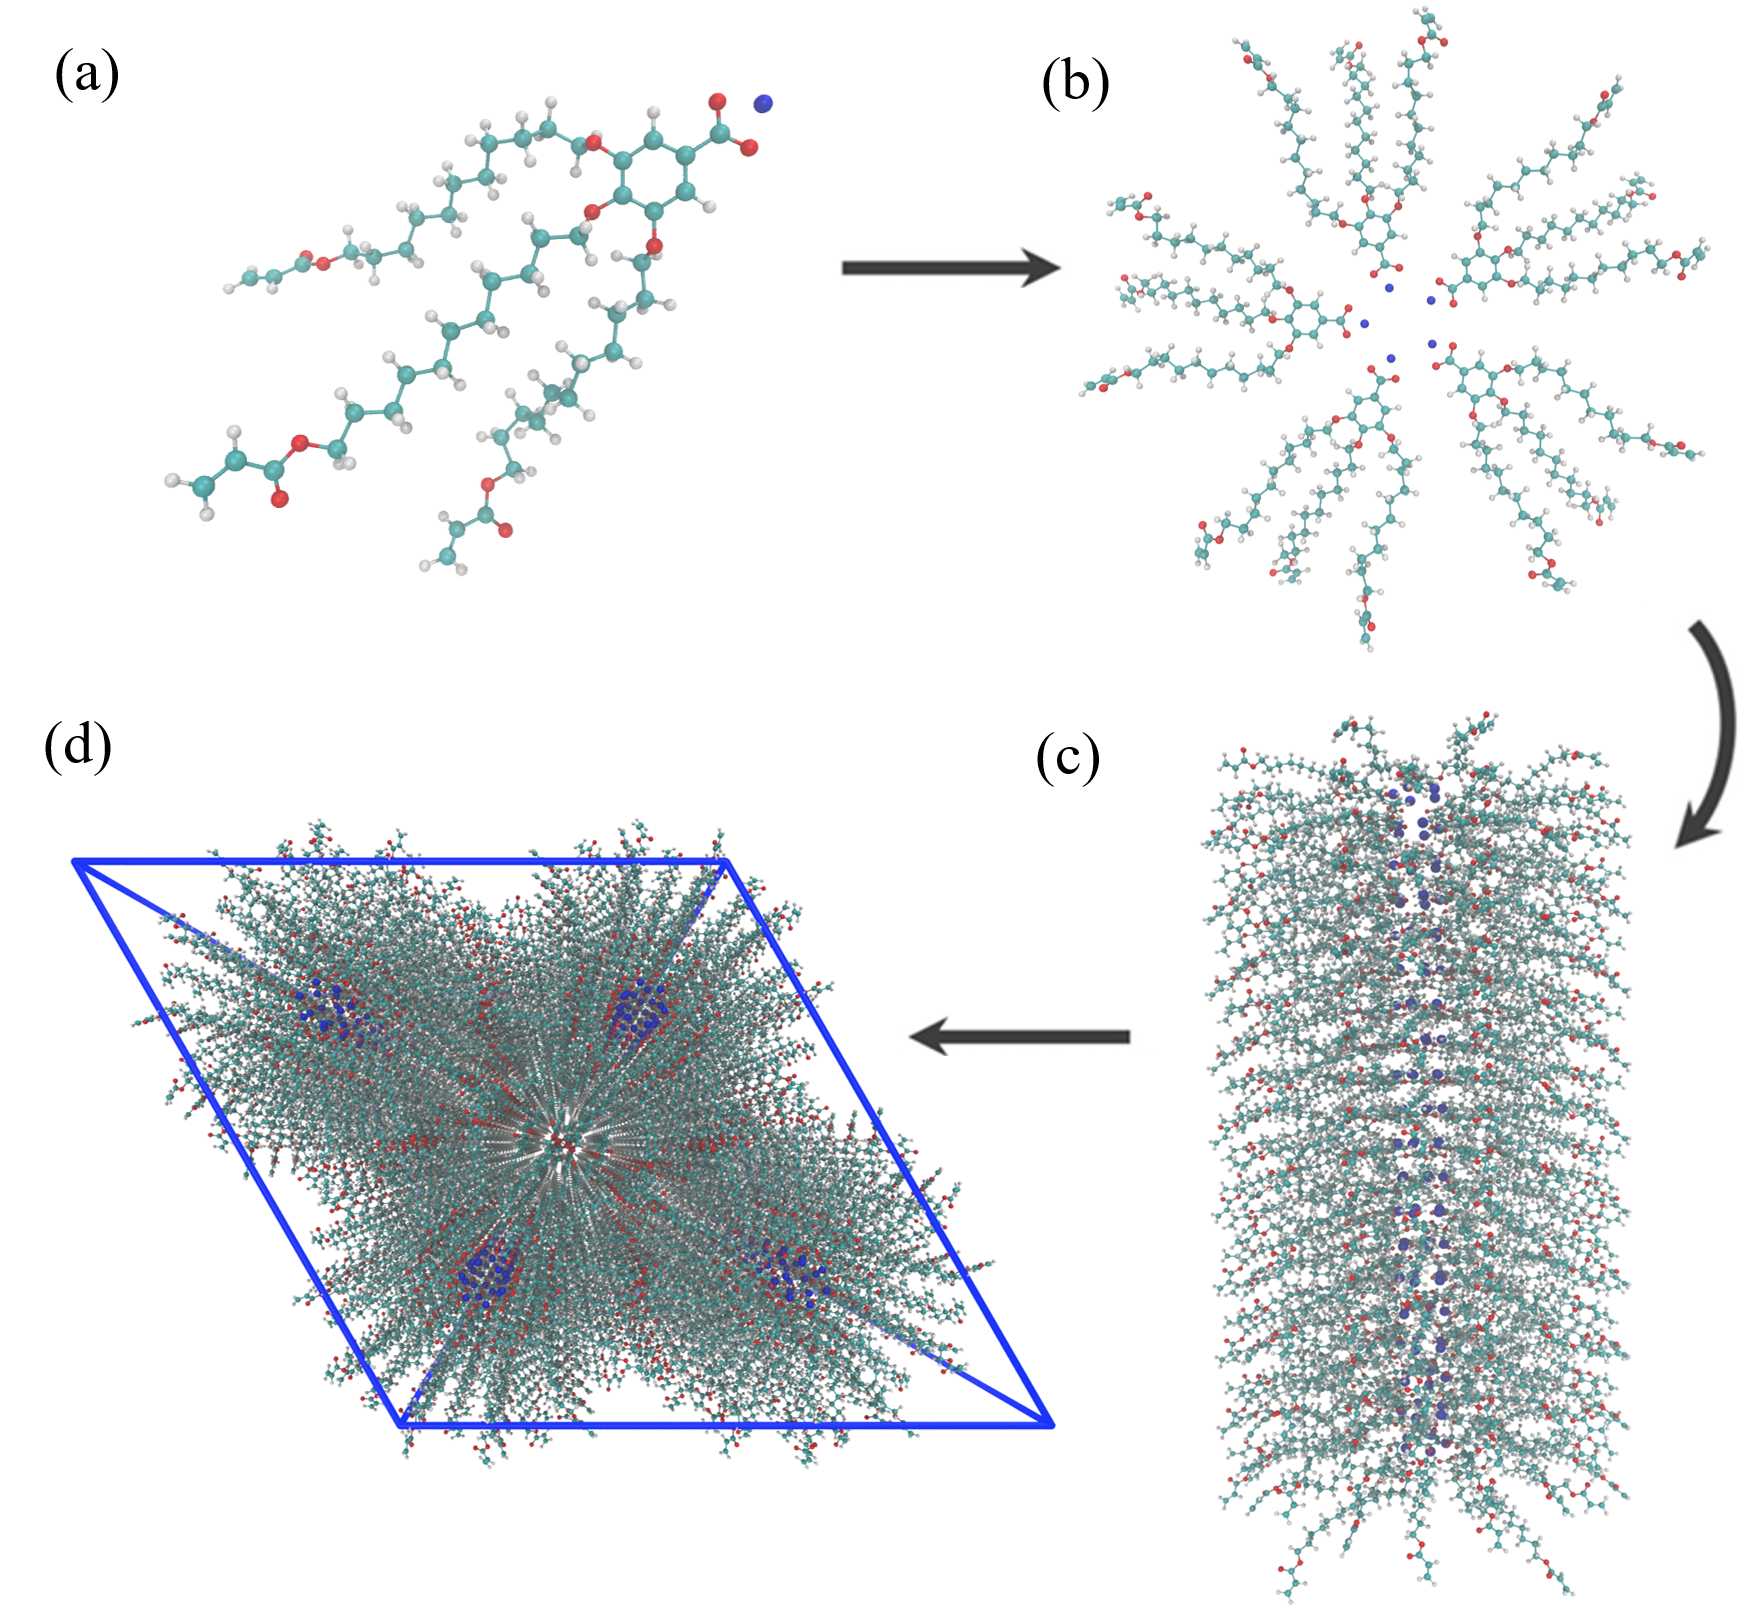
\includegraphics[width=0.75\linewidth]{build.PNG} %BJC: put an xyz axis with the unit cell
%	\caption{(a) We parameterized a single monomer and annealed it to produce a low energy
%		configuration. (b) A Python script assembles monomers into columns which are duplicated 
%		and rotated to surround hydrophilic pore centers. (c) We chose to stack twenty monomers
%		into each column. (d) The pores are duplicated and placed into a monoclinic unit cell.}\label{fig:python}
%  \end{figure}
  
  A typical simulation volume contains four pores in a monoclinic unit cell,
  the smallest unit cell that maintains hexagonal symmetry when extended
  periodically. Each pore is made of columns of stacked monomers with periodic
  continuity along the pore axis, avoiding any edge effects and creating an
  infinite length pore ideal for studying transport. We prefer a small number of stacked
  monomers in order to reduce computational cost and to allow us to look at
  longer timescales. Ultimately, we chose to build a system with 20 monomers
  per column in order to minimize finite size effects with reasonable computational expense 
  and to obtain sufficient resolution when simulating XRD patterns (see further discussion
  in section S-\ref{S-section:monomers_per_column}).
 
  \subsection{Monomer Placement} 

  When constructing an initial configuration, there are a number of variables
  which require careful consideration while placing monomers. The equilibrium
  configuration is sensitive to some while insensitive to others. We find the starting
  pore radius, defined as the distance of a chosen head group carbon from the
  pore's central axis, does not influence the equilibrium structure if one chooses
  a reasonable value. The pore radius is chosen to be 0.5 nm in our initial
  configurations. The initial distance between pores, within a wide range, also has 
  little effect on the the equilibrated structure. However, one should not start them
  too close or there will be high energy repulsions during early equilibration. We 
  chose an initial pore spacing of 4.5 nm, $\sim$10\% larger than the experimental value
  of 4.12 nm. A sensitivity analysis of both parameters is presented in the 
  %MRS13: be consistent on capitalization of ``Supporting'' ``Information'' and ``section''. Look at JPCB for guidance.
  Supporting information, section S-\ref{S-section:initial_config_dependence}. The 
  distance between vertically stacked monomers, the xy position of monomers with respect 
  to vertically adjacent monomers, and the number of columns per pore do influence the 
  equilibrated structure and require further justification for their choices. We rely on 
  experimental data to inform them. 

  We chose the vertical spacing between monomers for the initial configuration based
  on R-$\pi$ and then allowed the system to readjust during equilibration. We rotated 
  each monomer so the plane of its aromatic head group would be coplanar with the xy plane. We
  explored three different initial monomer spacings. The first is exactly
  equal to R-$\pi$ with layers placed so aromatic rings stack 3.7 \AA~apart in
  the z-direction. We also extensively explored a second system with an initial spacing of 5
  \AA. We briefly explored a third system with an initial spacing of 10
  \AA. However this largest spacing yields non-physical behavior which is detailed in the 
  Supporting Information, section S-\ref{S-section:initial_dbwl}. 

%  This is true if initial equilibration is performed with pressure control
%  If we initially space layers too far apart, they will collapse on each
%  other while simultaneously slipping in between layers of adjacent pores, which
%  leads to an artificially thick membrane with pores spaced closely together.
%  Further details of simulations with layer stacked 10 \AA apart are in the supplemental
%  information.

  We chose the relative orientation between vertically adjacent monomers in each column 
  based on clues from diffraction data as well as the various known stacking modes of 
  benzene and substituted benzene rings: sandwiched, parallel-displaced and T-shaped
  \cite{sinnokrot_estimates_2002}. We ruled out the T-shaped configuration
  because its $\sim$5 \AA~equilibrium stacking distance \cite{sinnokrot_estimates_2002}
  is inconsistent with R-$\pi$. It is also infeasible for the monomers to orient in the 
  T-shaped conformation because of the bulky tail groups. We explored the system's 
  preference towards the sandwiched vs. parallel displaced stacking modes in some detail.
  Both have reported stacking distances near the R-$\pi$ value of 3.7 \AA. Head groups in
  our sandwiched initial configuration stack directly on top of each other while
  head groups in the parallel displaced initial configuration stack with an offset
  of $180^\circ/ncol$ where $ncol$ is the number of columns per pore. See Figure 
  S-\ref{S-fig:stacking} for a detailed illustration of the initial configurations in each mode.
  
  % BJC5: figure here illustrating parallel displaced vs. sandwiched?

  The number of columns per pore is unknown, as stated in question
  (\ref{point:monomernum}). We tested configurations constructed with a varied
  number of columns per pore. We built systems in the sandwiched and parallel
  displaced configurations with 4, 5, 6, 7 and 8 monomers per layer.

  \subsection{Equilibration}\label{section:equilibration}
  We developed equilibration schemes for creating dry and wet configurations.
  Both schemes start with an initial configuration generated according to the
  previous guidelines. For wet systems, we added the desired concentration of
  water to the initial configuration and carried out equilibration in the same
  way as the dry systems. First, we fixed monomer head groups in place using
  position restraints with a force constant of 10$^6$ kJ mol$^{-1}$ nm$^{-2}$. We
  gradually released the position restraints by decreasing the force constants
  over a series of NVT simulations. We allowed the resulting unrestrained
  structure to equilibrate for 5 ns in the NPT ensemble with pressure controlled
  by the Berendsen barostat followed by NPT equilibration simulations run for at
  least 400 ns using the Parrinello-Rahman barostat. More equilibration details
  are given in section S-\ref{S-section:equilibration}.

  \subsection{Equilibrium Calculations}

  \subsubsection{\textit{Determining equilibration time}}\label{method:equil_time}

  Using equilibrated structures, we carried out various calculations to
  characterize the system. We defined the point at which a system is equilibrated
  based on when the distance between pores stopped changing.  We determined when
  the distances stopped changing by applying the statistical test of Chodera~\cite{chodera_simple_2016},
  implemented as \texttt{pymbar.timeseries.detectEquilibration}, to the time series. Typically, the pore-to-pore
  distance equilibrated between 200 and 350 ns. We used data collected after 
  equilibration to do all subsequent analysis.

  \subsubsection{\textit{Calculation of pore spacing}}\label{method:pore_spacing}

  To calculate the equilibrated pore spacing, we measured the distance between
  pore centers. We located the pore centers by averaging the coordinates of sodium
  ions in their respective pores. We generated pore spacing statistics 
  using the bootstrapping technique (See section S-\ref{S-section:p2p_stats} of the
  Supporting Information).

  %BJC5: moved to supporting info
  %BJC6: Do you think I should add this back since I used nematic order parameter to
  % differentiate between ordered/disordered basins?
  %MRS8: I think this is fine, since it's a relatively standard measure. 
% \subsubsection{\textit{The nematic order parameter}}\label{method:nematic_order}
%
%  We calculated the nematic order parameter for our system in order to
%  understand the degree of ordering among monomer head groups. Typically, the
%  nematic order parameter is calculated for nematic liquid crystal systems which
%  are characterized by unidirectional ordering of liquid crystal monomers. The
%  preferred direction of monomers is defined by the unit director vector,
%  $\mathbf{n}$. Assuming a single preferred direction of alignment, the nematic
%  order parameter, $S$, is defined as:
%  \begin{equation}
%	 S = \frac{1}{2} \langle(3\cos^2\theta -1)\rangle
%	\label{eqn:nematic_order_parameter}
%  \end{equation}
%  where $\theta$ is the angle between the molecular long axis and $\mathbf{n}$.
%  In a perfectly ordered system, the molecular axis should be aligned with
%  $\mathbf{n}$ and give an order parameter of $S=1$. We are interested in
%  quantifying the degree of monomer head group alignment between systems. We use
%  Eq.~\ref{eqn:nematic_order_parameter} to accomplish this by defining
%  $\mathbf{n}$ as the z-axis (or pore axis), and then measuring the angles,
%  $\theta$, between $\mathbf{n}$ and the vectors perpendicular to the plane of
%  the aromatic head groups. See the Supporting Information for a diagram.  

  \subsubsection{\textit{Generation of simulated X-ray diffraction patterns}}\label{method:xrd}
  
  %MRS13: I will talk to Matt about getting the code in GitHub.
  We generated simulated XRD patterns based on atomic coordinates in order to
  make a direct experimental comparison. We modeled all atomic coordinates as
  Gaussian spheres of electron density whose maximum and width are defined by
  each atom's atomic number electronic radius respectively. A three dimensional
  Fourier transform (FT) of the array of electron density results in a three
  dimensional structure factor which represents the unit cell in reciprocal
  space. The experimental WAXS measurement was made using a vertically aligned
  film whose pores were oriented perpendicular to the direction of the incident
  X-ray beam. 
  %BJC6: Below is the part I'm having a hard time putting into words. 
  Although the pores are vertically aligned, the crystalline domains are
  still misaligned with respect to the $xy$ plane. To account for this, we averaged
  2D slices of the structure factor at all angles about $|\mathbf{q}| = (0, 0, z)$. 

  We normalized all diffraction patterns relative to R-alkanes. We believe that
  the alkane-alkane density, averaged over all angles, is the feature most likely
  to be replicated between experiment and simulation, as atomistic alkane
  parameters are relatively well studied. Other features are dependent on system
  ordering which is likely to have some dependence on initial configuration.  We
  calculated the average intensity within R-alkanes of the experimental pattern,
  $I_{avg}$ and divided all intensities by this value. In this way, the average
  intensity of R-alkanes was equal to 1. When calculating $I_{avg}$, we excluded
  intensities within $\pm$ 30\degree~of the meridional axis defined by $q_r=0$,
  since the simulated patterns differ from experiment in those regions in all
  cases (See Figure~\ref{fig:ralkanes}). Specifically, in contrast to the
  experimental WAXS pattern, R-$\pi$, as it appears in the simulated diffraction
  patterns, intersects with R-alkanes (See Figure~\ref{fig:XRDsim}). We set an
  upper bound on the colorbar by multiplying $I_{avg}$ by a scaling factor, $f$.
  Intensities that appear in the patterns $\geq$ $f\times I_{avg}$ are colored
  uniformly.  We applied the same scaling method to the simulated patterns. We
  chose a scaling factor of $f=3.1$ in order to visibly display all
  features in all patterns.

%BJC12: redundant -- copied from methods
%  We developed standardized methods of measuring the intensity of reflections of interest
%  in the experimental and simulated X-ray diffraction patterns presented in this work. Here,
%  we graphically illustrate the methods used for measuring these intensities.

%  All diffraction patterns are normalized according to R-alkanes and the intensities
%  of all reflections are reported relative to the intensity of R-alkanes. The region
%  used to calculate the average intensity of R-alkanes is shown in
%  Figure~\ref{fig:ralkanes}. The top region is excluded because, in the simulated
%  patterns, R-$\pi$ intersects with R-alkanes.

  We reported the intensities of R-$\pi$ and R-double by recording the maximum values
  of the peaks of the $q_z$ cross-section of the experimental pattern at $q_r=0$ 
  (Figure~\ref{fig:rpi_rdouble}). In the case of the experimental pattern, the peak
  heights are not perfectly symmetrical, so we report the average of the two heights.

  We measured the intensity of R-spots by averaging the peak heights produced
  by radially integrating the patterns within the R-alkanes region
  (Figure~\ref{fig:rspots}).  In some patterns, the spots are not easily
  discernable due to obstruction by other features. In that case, we report the
  average intensity at the intersection of R-alkanes with the $q_z$ value of
  R-double since that is where we expect it to appear based on experiment. Since
  R-double does not appear in our simulated patterns, we estimate where it should
  appear as half of the $q_z$ value of R-$\pi$.

 % We measured the intensity of R-spots by calculating the average intensity
 % within a region selected by visual inspection. We report the average intensity
 % within the regions highlighted in red in Figure~\ref{fig:rspots}. 

  We measured the intensity of R-pores based on the intensity of the
  d\textsubscript{100} peak (the leading peak closest to $q_r$ = 0) of the $q_r$
  cross-section of the patterns at $q_z$=0 (Figure~\ref{fig:saxs_xsection}). The
  beamstop covers most of the small angle reflections in the experimental 2D WAXS
  pattern. In order to compare the simulated intensity of R-pores to experiment,
  we used the $q_r$ cross-section of 2D SAXS which was generated from the same
  sample (Figure S-\ref{S-fig:2DSAXS}). Since the d\textsubscript{200} peak is
  partially exposed in the experimental 2D WAXS pattern, we normalized the
  experimental 2D SAXS cross-section by matching the intensity of the
  d\textsubscript{200} peak between it and the experimental 2D WAXS
  cross-section. It is possible that the peak is not fully captured in the 2D
  WAXS pattern and that we have underestimated the intensity of R-pores in the
  experimental pattern.     

  \begin{figure}[!htb]
  \centering
  \begin{subfigure}{0.45\linewidth}
  \centering
  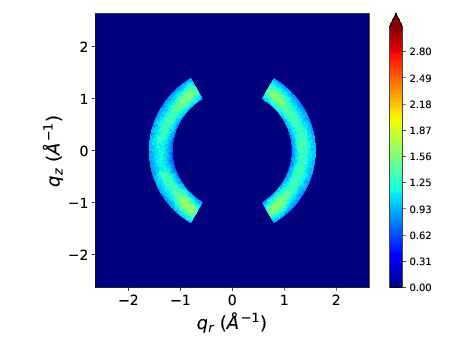
\includegraphics[width=\textwidth]{ralkanes.png}
  \caption{R-alkanes}\label{fig:ralkanes}
  \end{subfigure}
  \begin{subfigure}{0.45\linewidth}
  \centering
  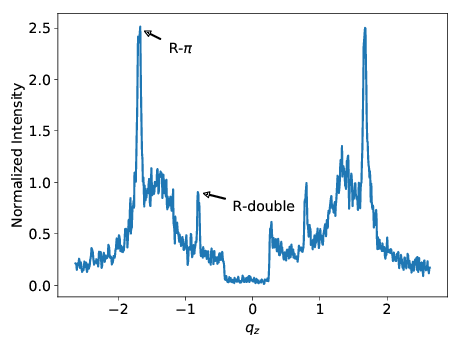
\includegraphics[width=\textwidth]{rpi_rdouble.png}
  \caption{$q_z|_{r=0}$}\label{fig:rpi_rdouble}
  \end{subfigure}
  \begin{subfigure}{0.45\linewidth}
  \centering
  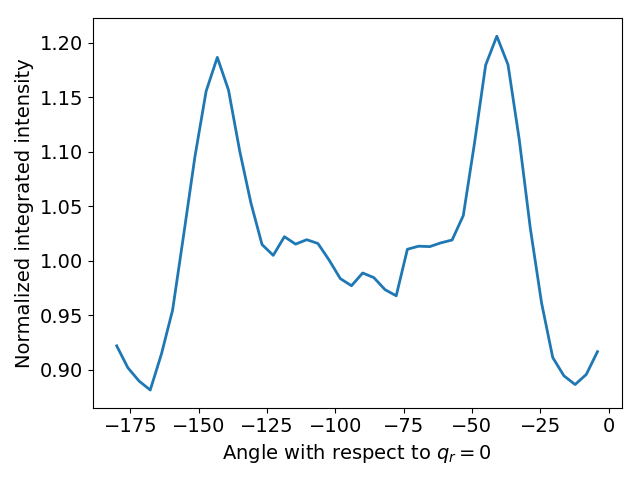
\includegraphics[width=\textwidth]{angular_integration.png}
  \caption{R-spots}\label{fig:rspots}
  \end{subfigure}
  \begin{subfigure}{0.45\linewidth}
  \centering
  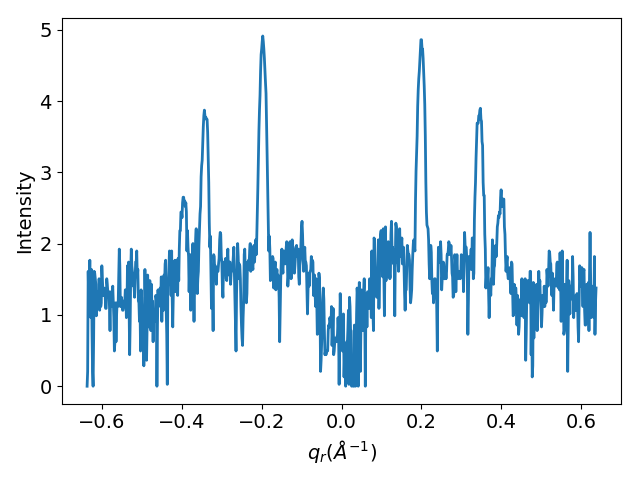
\includegraphics[width=\textwidth]{saxs_xsection.png}
  \caption{R-spots}\label{fig:saxs_xsection}
  \end{subfigure}
  \caption{(a) We measured the intensity of R-alkanes by calculating the average 
  intensity within the region bounded by $|\mathbf{q}|$ = 1.4~$\AA^{-1}$ and 
  1.57~$\AA^{-1}$ (between 4.0 and 4.5 \AA~in real space). We excluded intensities
  within $\pm$ 30\degree~of the meridional axis defined by $q_r=0$, since the 
  simulated spectra overlap with R-$\pi$ in that region. in those regions in all cases. (b) We
  measured the intensity of R-$\pi$ and R-double based on the peaks of the $q_z$
  cross-section of the diffraction pattern. (c) We measured the intensity of R-spots
  by averaging the peak heights produced by radially integrating the patterns within 
  the R-alkanes region. We took the intensity of R-spots as the average of the 
  peak intensities near 37 and 143$\degree$. (d) We measured the intensity of 
  R-pores by measuring the height of the d\textsubscript{100} peak (the leading
  peak closest to $q_r$=0) of the cross-section of the diffraction patterns along
  the $q_r$ axis at $q_z$=0.} \label{fig:xrd_intensities}
  %MRS13: it's confusing to have the same label (R-spots) beneath c and d.  Should be different labels if different data.
  \end{figure}
 
  \subsubsection{\textit{Pair distribution functions and correlation length}}\label{section:correlation_length}

  The normalized pair distribution function, $g(\mathbf{r})$, describes
  the probability of finding a pair of particles separated by $\mathbf{r}$,
  \begin{equation}
	g(\mathbf{r})= \frac{1}{\rho N} \Bigg \langle \sum_{i=1}^{N}\sum_{j\neq i}^{N} \delta(\mathbf{r}+\mathbf{r_j}-\mathbf{r_i}) \Bigg \rangle
	\label{eqn:correlation}
  \end{equation}
  where $\rho$ is the average number density of particles and
  $\delta(\mathbf{r})$ is the Dirac delta function\cite{kuriabova_linear_2010}.
  We applied equation \ref{eqn:correlation} in three dimensions and then
  extracted one dimensional distribution functions using slices of the grid
  along the appropriate axis.

  We measured the one dimensional pair distribution function, $g(z)$, between centers 
  of masses of aromatic head group rings along the z-axis (perpendicular to
  the membrane plane). We averaged all 1D $z$-directional slices of the full 3D 
  correlation function within 2.1~\AA~of $(x, y)=(0, 0)$. We chose 2.1 \AA~as a crude 
  approximation of the radius of the phenyl ring plane. 
  %In this way, we include any instances of 
  %overlapping electron density which would contribute to R-$\pi$. 
  We calculated the radius as the sum of the longest C-C distance within a phenyl 
  ring (2.8~\AA) and two times the carbon atom radius (0.7~\AA). % citation
  
  Here, $g(z)$ is characterized by an oscillatory function with a period equal to the
  average distance between stacked monomers, and an amplitude that decays exponentially
  (see Figure~\ref{fig:correlation}). The rate of decay is related to the correlation 
  length, L, between monomer head groups. We estimated L by fitting the peaks of $g(z)$
  %MRS13: I assume a linear least squares fit?  Be precise so it's reproducible.
  to a decaying exponential function of the form:
  \begin{equation}
  	Ae^{-z/L}
  	\label{eqn:decaying_exponential}
  \end{equation}
  where A is a fitting parameter for amplitude, $z$ is the independent variable of $g(z)$ 
  and L is the fit correlation length. We calculated the error in the estimated value
  of L as the square root of the diagonal entry of the covariance matrix of 
  optimized fit parameters.  %BJC6: reference scipy curve_fit?
  
  We also used $g(z)$ to calculate the equilibrated vertical stacking distance between
  monomers, $d_{equil}$. 
  %BJC5: in case there is an criticism of this method
  %The simplest way to do so, would be to Fourier transform
  %$g(z)$ and extract the highest amplitude frequency of the resulting Fourier series. 
  %However, the size of our system limits the width of the bins in Fourier space. The bins
  %are too large to extract a precise value of $\mathit{d}_equil$. Instead, 
  We fit a decaying sinusoidal function to $g(z)$ of the form:
  \begin{equation}
  	1 - A\cos\left(\frac{2\pi}{\mathit{d}_{equil}}z + B\right)e^{-z/L}
  	\label{eqn:decaying_sinusoid}
  \end{equation}
  where A and B are fit parameters for the function's amplitude and phase shift respectively.
  This function could be used in place of Equation~\ref{eqn:decaying_exponential}, however
  it does not consistently fit the peaks of $g(z)$ from parallel displaced configurations 
  well enough to extract a reliable value of L.
  %BJC5: maybe include plots of these fits in supporting info

% BJC5: I don't plan on showing any 2D correlation functions -- maybe to show swelling
% of solvated systems.

%  In two dimensions, we observed xy and xz pair distribution functions based on
%  the center of masses of the aromatic head group rings. For the xy pair
%  distribution functions, we used a rotated frame of reference. For a given center
%  of mass, we rotated the coordinates so that the vector created from the center
%  of mass to the pore center was aligned with the positive x-axis. 

  %We gave special
  %consideration to the xy cross-sections since multiple rings exist in the same
  %plane located at different vertices of a polygon. We used a rotated frame of
  %reference to avoid ambiguity in the final pair distribution functions. i

  \subsection{Simplified Systems}\label{method:simple_systems}
  
  In order to gain a deeper understanding of discrepancies between the experimental and
  and simulated R-$\pi$ reflection, we used a simplified model where we 
  represent each monomer as a single point scatterer located at the center of mass
  of its head group. In order to make a system approximately similar to our equilibrated 
  simulation geometries, we created 4 hexagonally packed pore regions spaced 42.5 \AA~ 
  apart, each with 5 columns of scatterers spaced 4.4 \AA~apart in the $z$-direction. We
  built the system 4 times taller in the $z$-direction (80 scatterers per column) in order
  to access higher $q_z$ resolution.
  
  We gave the simplified models the same amount of disorder present in the atomistic
  simulations. We observe two sources of disorder: thermal motion of atoms
  and quenched disorder which is created by rapid structural rearrangement during 
  early equilibration and is largely locked into place for the remainder of the 
  simulation. We measured thermal disorder by calculating the standard deviation of 
  the distribution of head group center of mass positions from their average positions.
  We measured quenched disorder by calculating the standard deviation of the distribution
  of head group center of masses from their idealized average positions. In the 
  $z$-direction, we measured the deviation of the head group center of masses from an
  equally spaced column of head groups. In the $xy$ plane, we calculated the standard 
  deviation in radial position from the pore center and the angular deviation from 
  equally spaced points surrounding the pore center. This method for calculating 
  quenched order inherently includes thermal disorder. 
  
  We approximated interactions between particles by correlating the $z$-distance 
  between points within each column of point scatterers. We placed points in each
  column by drawing random samples from a multivariate normal distribution defined
  by the mean positions of an equally spaced column of points. We gave the 
  distribution at each point along the column the same standard deviation, 
  $\sigma_z$ and we defined a covariance matrix such that the covariance, $v$, of
  the distance, $d$, between scatterers decays exponentially from $v$ according
  to the equation $ve^{-d/L}$, where $L$ is the correlation length. Unless noted
  otherwise, we used the experimental correlation length of 9.0 \AA. 
  
  We calculated averaged R-$\pi$ profiles by simulating the diffraction pattern
  of trajectories consisting of 1000 independent simple system configurations 
  generated with point scatterer placement based on the quenched order seen in
  atomistic simulations. The quenched disorder is greater in  magnitude than thermal 
  disorder (See Table~\ref{table:quenched_disorder} in section~\ref{section:rpi}).
  %MRS13: you just said this already, commenting out.
  %and inherently includes thermal disorder due to the way we calculate it.
  This method assumes that the timescales for large scale rearrangements of the
  system are much longer than what we can feasibly simulate.

  \subsubsection{\textit{Radial distribution functions}}

  We explored the pores' compositions by measuring the average number densities
  of various monomer components as a function of distance from the pore centers.
  We looked at the average number density of sodium ions, aromatic rings and 
  carbon atoms making up the monomer tails. We binned the radial distance of all
  atoms in each group from the pore centers, then normalized by the volume of the
  annulus defined by the bin edges and the z box vector (See Figure~S-\ref{S-fig:rdf_diagram}). 

  \subsubsection{\textit{Ionic conductivity calculations}}

  We calculated ionic conductivity using the Nernst-Einstein relationship, which 
  relates the DC ionic conductivity, $\sigma$, to ion diffusivity, $D$, 
  concentration, $C$, ion charge, $q$, the Boltzmann constant, $k_b$, and 
  temperature, $T$: 
  \begin{equation}
	\sigma = \dfrac{q^2CD}{k_b T} 
	\label{eqn:nernst_einstein}
  \end{equation}
  We measured sodium ion diffusion coefficients by calculating the slope
  of the linear region of the $z$-direction mean square displacement curve as
  indicated by the Einstein relation \cite{einstein_investigations_1956}. We
  visualized the MSD plot to determine where to begin and end a linear fit. We
  measured ion concentration with respect to the volume of the entire unit cell. 
  More details are provided in the Supporting Information, Section~S-\ref{S-section:ionic_conductivity}.

  \subsection{Cross-linking}
  
  In order to better match the experimental membrane synthesis process,
  we created a cross-linking algorithm that one can apply to equilibrated structures. 
  The primary purpose of cross-linking is to create a mechanically robust membrane.
  For that reason, we are not concerned with replicating the kinetics of the reaction, 
  but instead emphasize understanding how much and in what way cross-linking modulates
  the system's structure.

  We based our cross-linking algorithm on the known reaction mechanism 
  (Figure S-\ref{S-fig:xlink_mech}). The reaction takes place at the terminal vinyl groups
  on each alkane tail. The procedure is carried out iteratively. Each iteration, the
  algorithm chooses carbons to cross-link based on the distance between eligible 
  carbon pairs. The algorithm then updates the topology with the new bonds and atom
  types, energy minimizes the system and runs a short simulation before selecting 
  the next group of eligible carbons atoms.

  \section{Results and Discussion}
  
  \subsection{Density of monomers around pores}\label{section:mon_per_pore}

% BJC5: old
%  Our simulations best support a model built with 5 monomers per layer based on
%  the measured equilibrated pore-to-pore distances. To discern the composition of
%  the monomer layers, addressing question (\ref{point:monomernum}), we ran
%  simulations of systems created with 4--8 monomers per layer. We built systems
%  in both the parallel displaced and sandwiched configurations with layers
%  initially spaced 3.7 \AA~apart. We prepared equilibrated configurations
%  according to the dry equilibration procedure. The pore-to-pore spacing is stable
%  in all systems are stable after 400 ns of simulation. Figure~\ref{fig:p2p} shows
%  the equilibrated pore-to-pore distances for all systems tested. Systems built 
%  with 5 monomers in each layer equilibrate to a pore spacing that is most consistent
%  with the experimental value of 4.12 nm derived from SAXS measurements 
%  (Figure~\ref{fig:SAXS}).
%  
%  The remainder of this discussion will focus on the analysis of systems built with
%  5 monomers per layer. Systems built with 6 monomers per layer have an equilibrated
%  pore spacing c.a. 0.50 nm higher than experiment. Systems built with 4 monomers per 
%  layer equilibrate to a pore spacing 0.25 nm lower than experiment. In a sense, all
%  systems tested are at least metastable, however not all will make physical
%  sense or fit the experimental profile that we are trying to match. In the limit of
%  infinite time, all simulations will converge to a single density. It is our 
%  intention to choose an initial configuration which quickly reaches a monomer density
%  close to experiment.   
  
  Our simulations best support a model built with 5 monomer columns per pore based on
  the measured equilibrated pore-to-pore distances. To discern the composition of
  the monomer layers, addressing Question \ref{point:monomernum} above, we ran
  simulations of systems created with 4--8 columns per pore. We built systems in both
  the parallel displaced and sandwiched configurations and equilibrated them according
  to the dry equilibration procedure. We tested all systems with an initial vertical monomer 
  spacing, $\mathit{d}$, of 3.7 \AA~in accordance with R-$\pi$. We tested 4 additional 
  systems with monomers initially spaced 5 \AA~apart vertically (see section~\ref{S-section:initial_pore_spacing}
  of the Supporting Information for more details on sensitivity to initial layer spacing). 
  We considered the pore-to-pore spacing to be equilibrated as defined in section~\ref{method:equil_time}.
  Figure~\ref{fig:p2p} shows the equilibrated pore-to-pore distances for all systems tested. 
  
  \begin{figure}[!htb]
	\centering
	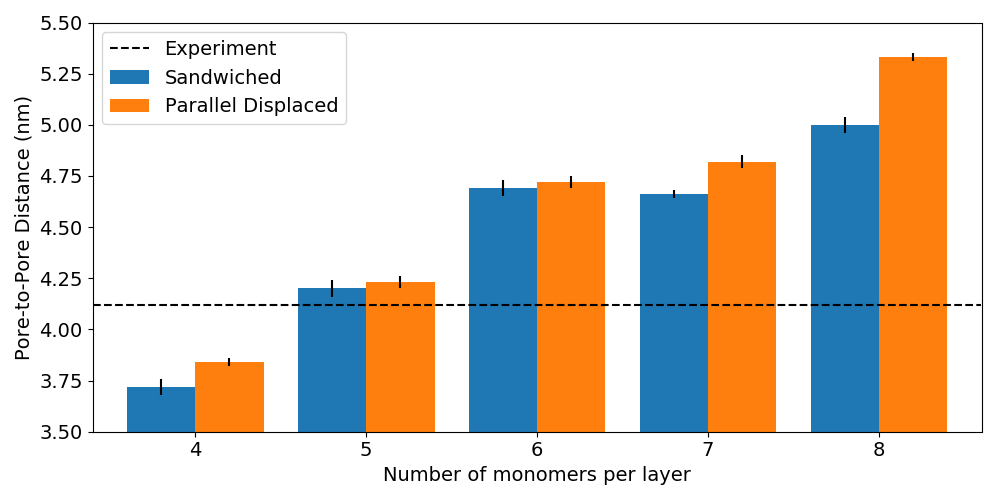
\includegraphics[width=\linewidth]{p2p.png}
	\caption{Systems with 5 columns per pore have equilibrated pore spacings closest to
			 the experimental value of 4.12 nm. The equilibrated pore spacing of the model 	
			 increases as the number of columns in each pore increases.}~\label{fig:p2p}
  \end{figure}  
  
  All systems tested, although equilibrated from the perspective of the metrics used here, are
  frozen in metastable basins. Not all make physical sense or fit the experimental profile that 
  we are trying to match. In the limit of infinite simulation time, all systems will in theory 
  converge to a single equilibrium configuration, but that time is far beyond the 100's of 
  nanosecond simulated here. For simplicity, we group the systems studied here into the ordered
  and disordered basins. What we find is that any system where $\mathit{d}=3.7$ \AA~can generally 
  be characterized as being in a more ordered basin, and any system where $\mathit{d}=5.0$ \AA~can
  be characterized as a more the disordered basin. Generally, when monomers are started further 
  apart, they stay further apart than systems where monomers are started closer together 
  (see Table~\ref{table:correlation_length}). Because of the extra space between stacked 
  monomers, monomer head groups have more rotational freedom. We quantified the ordering of
  the head groups using the nematic order parameter (see section S-\ref{S-method:nematic_order}
  for details of calculation). Disordered basin systems have a lower nematic order parameter 
  (meaning they are more disordered) than ordered basin systems.

  %MRS7: maybe above say where (i.e. what section) it will become clear?  Or possibly describe them here by order parameter instead of by starting distance, and state the correlation between starting distance and order parameter.
%    All systems tested are at least metastable on the timescales studied here, however not all 
%  make physical sense or fit the experimental profile that we are trying to match. In the limit
%  of infinite simulation time, all simulations will converge to a single density. It is our 
%  intention to choose an initial configuration which quickly reaches a monomer density close 
%  to experiment. We believe systems built with 5 columns per pore achieve this goal.
  
  Systems built with 5 columns in each pore equilibrate to a pore spacing that
  is most consistent with the experimental value of 4.12 nm derived from SAXS
  measurements (Figure~\ref{fig:SAXS}). Ordered basin systems built with 4
  columns per pore equilibrate to an average pore spacing 0.25 nm lower than
  experiment. Ordered basin systems built with 6 columns per pore, have an
  equilibrated pore spacing ca. 0.50 nm higher than experiment.  Monomers in
  disordered basin systems built with 6 columns-per-pore agree with experimental
  pore-to-pore distances within error, but stack too far apart. Those in the
  disordered sandwiched and disordered parallel displaced configurations stack
  $\sim$~4.87 and 4.94 \AA~apart respectively, which is ca. 1.2~\AA~further apart
  than suggested by experiment. 5 column-per-pore systems stack, at a maximum,
  0.9 \AA~further apart than experiment (see 
  Table~\ref{table:correlation_length}).  The remainder of this discussion will
  focus on the analysis of systems built with 5 columns per pore. 

% BJC6: I don't think I need to say the following in above paragraph since its all in the methods.
% Our methodology for calculating equilibrium stacking distance is fully explained in section~\ref{section:rpi}.
% MRS8: sounds good.  
%  Relative to ordered basin 
%  6 column-per-pore systems, the unit cell is elongated in its z dimension and contracted in its
%  x and y dimensions, however the box volume stays nearly constant in all cases 
%  (Figure~\ref{fig:box_dimensions}). The system is likely not fully equilibrated and may eventually
%  rearrange into something that resembles a 5 column-per-pore system. Further investigations 
%  into this are beyond the scope of this paper.

%  \begin{figure}[!htb]
%  \centering
%  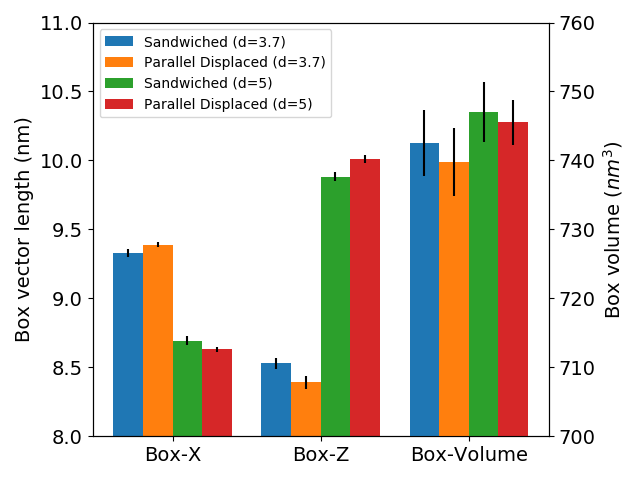
\includegraphics[width=\textwidth]{box_dimensions.png}
%  %MRS7: not really clear from the caption why this is shown.
%  \caption{When monomers are initially stacked 5 \AA~apart ($\textit{d}=5~\AA~$), the unit cell
%  expands in the z direction and contracts in its x and y dimensions. The volume remain nearly
%  constant across all cases. The y dimension box vectors are not included since we use 
%  semiisotropic pressure coupling which requires that the x and y box vectors change uniformly.}\label{fig:box_dimensions}
%  \end{figure}  
  
  \subsection{Simulated XRD comparison to 2D WAXS data}
  
  We can better understand the structure of the system by simulating X-ray
  diffraction patterns produced from equilibrated MD trajectories (see
  section~\ref{method:xrd}) and comparing them to experiment, addressing
  Question~\ref{point:xrdmatch}. We tested systems built with 5 columns per pore
  in the parallel displaced and sandwiched configurations at
  300 K in the ordered and disordered basins, as those were the most consistent
  with the most unambiguous X-ray diffraction features, the pore-to-pore spacing
  and the stacking distance.  We generated simulated patterns using the locally
  equilibrated portion of each simulation trajectory (See
  Section~\ref{method:equil_time}). There are two important factors to take into
  account when looking at differences between experimental XRD and simulated XRD.
  First, the simulated diffraction patterns have some noise, especially along the
  $q_z$ axis at $q_r$=0, which is where several of the more interesting features
  are located. This is due to the angle averaging of the 3D structure factor
  around the $q_z$-axis, meaning there are fewer samples as  $q_r$ approaches 0.
  The amount of samples required to to converge along the $q_z$ axis is analyzed
  in Supporting Information section S-\ref{S-section:xrd_noise}.  More
  importantly, our simulations do not appear to be long enough to sample truly
  independent configurations within their respective metastable basins (see
  section~\ref{section:slow_dynamics}), meaning we must take care in interpreting
  the results of the XRD. The simulated patterns generated for all systems
  studied are shown and compared to experiment in Figure~\ref{fig:XRDsim}.

  % BJC10: to be reformatted : add captions. Maybe shift experimental pattern to (a)
  % BJC10: be more terse in main caption. Add references to sections
  \begin{figure}[!htb]
	\centering
	\begin{subfigure}{0.88\textwidth}
	\begin{subfigure}{0.28\linewidth}
			\begin{subfigure}{\textwidth}
			\centering
		        	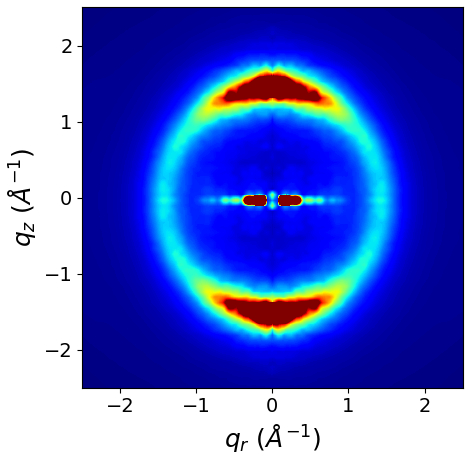
\includegraphics[width=\linewidth]{rzplot_layered_300K_jet_nocbar.png}
			\end{subfigure}
			\begin{subfigure}{\textwidth}
		       		\centering
	        		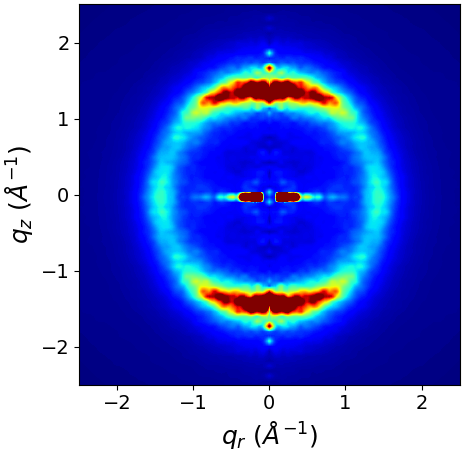
\includegraphics[width=\linewidth]{rzplot_layered_300K_disorder_jet_nocbar.png}
			\end{subfigure}
	\end{subfigure}
	\begin{subfigure}{0.4\linewidth}
	\centering
			\begin{subfigure}{\textwidth}
		       		\centering
	        		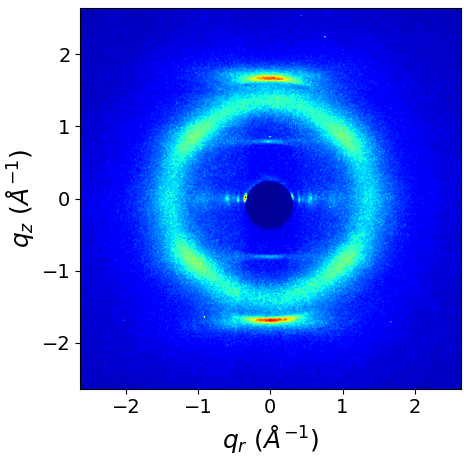
\includegraphics[width=\linewidth]{WAXS_raw_jet_nocbar.png}
			\end{subfigure}
	\end{subfigure}
	\begin{subfigure}{0.28\linewidth}
	\centering
			\begin{subfigure}{\textwidth}
			\centering
		        	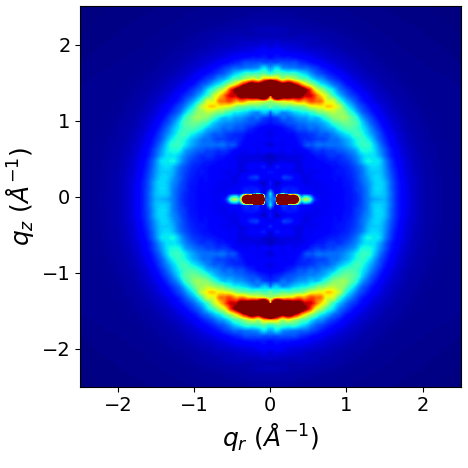
\includegraphics[width=\linewidth]{rzplot_offset_300K_jet_nocbar.png}
			\end{subfigure}
			
			\begin{subfigure}{\textwidth}
				\centering
			    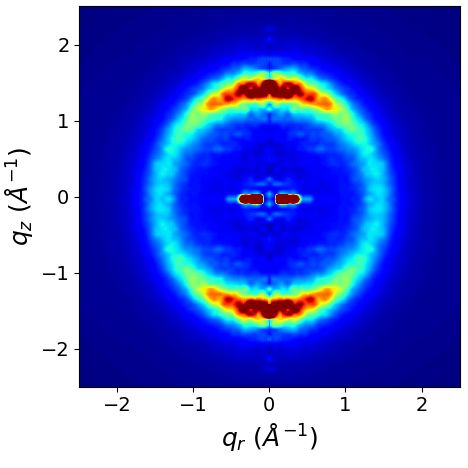
\includegraphics[width=\linewidth]{rzplot_offset_300K_disorder_jet_nocbar.png}
			\end{subfigure}
	\end{subfigure}
	\end{subfigure}
	\begin{subfigure}{0.1\textwidth}
		\centering
		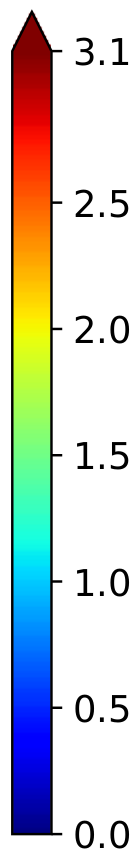
\includegraphics[width=\linewidth]{colorbar_jet.png}
	\end{subfigure}	
	\caption{Simulated XRD patterns show some qualitative agreement with
		experiment. Shown is a comparison of the (a) Sandwiched, ordered basin (b)
		Sandwiched, disordered basin (d) Parallel displaced, ordered basin and (e)
		Parallel displaced, disordered basin configurations with (c) experimental WAXS.
		The major reflections of interest (See Figure~\ref{fig:SWAXS} for their
		definitions) are present at varying degrees. In all cases, R-pores, R-alkanes
		and R-$\pi$ are present to some degree. R-spots is also present, however it is
		generally partially covered by the broad R-$\pi$ reflection. Quantitative
		comparisons of the relative intensities and locations of reflections of
		interest are presented in Table~\ref{table:relative_intensities_300K}. In both
		XRD patterns generated from parallel displaced patterns, there is a faint line
		across $q_z \sim 0.7~$\AA$^{-1}$, half the simulated value of R-$\pi$. Although
		it does not cross through $q_r = 0$~\AA$^{-1}$, it is at the same $q_z$ value
		where we expect R-double to be present. Still, R-double is not fully reproduced
		in any of the simulated patterns.}~\label{fig:XRDsim} 
  \end{figure}
  
  The simulated XRD patterns show moderate agreement with experiment. There 
  are key qualitative and quantitative differences between the experimental and simulated
  locations and intensities of each major reflection. The integrated intensity and location
  of each simulated reflection relative to its experimental counterpart are shown in  
  Table~\ref{table:relative_intensities_300K}. Our approach for measuring the intensity of
  each reflection is described in Section~\ref{method:xrd}. 
  %MRS12: should that be in Methods instead of suporting?  Not sure.
  %BJC12: moved into methods for now. 

  In the next few subsections, we individually address each major reflection, and the
  similarities and differences between simulation and experiment. We start with relatively 
  uncomplicated analyses of reflections that are very similar between experiment and simulation:
  \begin{itemize}
  	\item The location of R-alkanes (section~\ref{section:ralkanes})
  	\item The location and intensity of R-pores (section~\ref{section:rpores})
  \end{itemize}
  and then move onto more complicated explanations of those reflections whose characteristics
  do not match, or have not been fully explained by experiment:
  \begin{itemize}
  	\item The origin of R-spots (section~\ref{section:rspots})
  	\item The position, shape and intensity of R-$\pi$ (section~\ref{section:rpi})
  	\item The origin of R-double (section~\ref{section:rdouble})
  \end{itemize}
  
%  \begin{table}[h]
%  \centering
%  \begin{tabular}{c|cccccccccc}
%  \toprule
% 		   & \multicolumn{5}{c}{Configuration} \\
%  \hline
%           &\multicolumn{2}{c}{}            & \multicolumn{2}{c}{}          & \multicolumn{2}{c}{Parallel} & \multicolumn{2}{c}{Disordered} & \multicolumn{2}{c}{Disordered}         \\
%           & \multicolumn{2}{c}{Experiment} & \multicolumn{2}{c}{Sandwiched} & \multicolumn{2}{c}{Displaced} & \multicolumn{2}{c}{Sandwiched}  & \multicolumn{2}{c}{Parallel Displaced} \\
%  Reflection & Intensity & Location ($\AA^{-1}$) & Intensity & Location ($\AA^{-1}$) & Intensity & Location ($\AA^{-1}$) & Intensity & Location ($\AA^{-1}$) & Intensity & Location ($\AA^{-1}$) \\
%  \midrule
%  R-alkanes  & 1.0  & 1.4  & 1.0  & 1.4 & 1.0 & 1.4 & 1.0 & 1.4 & 1.0 & 1.4  \\  
%  R-spots    & 1.3  & 1.4  & 1.3  & 1.4 & 1.2 & 1.4 & 1.1 & 1.4 & 1.2 & 1.4  \\
%  R-$\pi$    & 2.8  & 1.7  & 44.0 & 1.4 & 7.7 & 1.4 & 8.4 & 1.4 & 10.1& 1.4  \\
%  R-double   & 0.9  & 0.85 & --   &  -- & --  & --  & --  & --  &  -- & --   \\ 
%  \bottomrule
%  \end{tabular}
%  \caption{The simulated XRD patterns of the systems tested, normalized so that the average 
%  intensity of R-alkanes equals 1, show R-$\pi$ reflections that are significantly higher 
%  than experiment and R-spots reflections that are slightly lower than experiment. R-double
%  does not appear in any patterns, and thus has no measurable intensity.}
%  \label{table:relative_intensities_300K} 
%  \end{table}
  
  \begin{table}[h]
  \centering
  \begin{tabular}{c|ccccc}
  \toprule
 		     & \multicolumn{5}{c}{Normalized Reflection Intensity}                   \\
  \hline
             &            &            & Parallel  & Disordered & Disordered         \\
  Reflection & Experiment & Sandwiched & Displaced & Sandwiched & Parallel Displaced \\
  \midrule
  R-alkanes  & 1.0        &  1.0       &  1.0      &  1.0       &  1.0               \\
  R-pores    & 4.91       & 49.5       & 54.0      & 50.8       & 53.4               \\
  R-spots    & 1.2        &  1.2       &  1.2      &  1.1       &  1.1               \\
  R-$\pi$    & 2.8        & 44.0       &  7.7      &  8.4       & 10.1               \\
  R-double   & 0.9        &  --        & --        &  --        & --                 \\ 
  \hline
   		     & \multicolumn{5}{c}{Reflection Location ($|\mathbf{q}|~\AA^{-1}$)}     \\
  \hline
             &            &            & Parallel  & Disordered & Disordered         \\
  Reflection & Experiment & Sandwiched & Displaced & Sandwiched & Parallel Displaced \\
  \midrule
  R-alkanes  & 1.39       &  1.44      &  1.44     & 1.42       & 1.43               \\  
  R-pores    & 0.176      &  0.170     &  0.170    & 0.173      & 0.172              \\
  R-spots    & 1.39       &  1.44      &  1.44     & 1.42       & 1.43               \\
  R-$\pi$    & 1.70       &  1.41      &  1.42     & 1.40       & 1.40               \\
  R-double   & 0.85       &  --        & --        &  --        & --                 \\ 
  \bottomrule
  \end{tabular}
  %MRS12: question: is the normalization for the simulated systems the same, no matter if disordered, etc.  If not chosen to be exactly the same, how different are they?
  %BJC12: Are you asking what the normalization constant is that I divide the patterns by for each system? I'll have to check. 
  \caption{The simulated XRD patterns of the systems tested, normalized so that
	  the average intensity of R-alkanes in each pattern equals 1, show R-pores and
	  R-$\pi$ reflections that are significantly higher than experiment and R-spots
	  reflections that are slightly lower than experiment. R-double does not appear
	  in any simulated patterns, and thus has no measurable intensity.}
  \label{table:relative_intensities_300K} 
  \end{table}  
  
%    \begin{table}[h]
%  \centering
%  \begin{tabular}{c|ccccc}
%  \toprule
% 		   & \multicolumn{5}{c}{Configuration} \\
%  \hline
%             &\multicolumn{2}{c}{}     &            & Parallel  & Disordered & Disordered         \\
%  Reflection & \multicolumnExperiment & Sandwiched & Displaced & Sandwiched & Parallel Displaced \\
%  \midrule
%  R-alkanes  & 1.0        &  1.0       &  1.0      & 1.0        & 1.0                \\  
%  R-spots    & 1.3        &  1.3       &  1.2      & 1.1        & 1.2                \\
%  R-$\pi$    & 2.8        & 44.0       &  7.7      & 8.4        & 10.1               \\
%  R-double   & 0.9        &  --        & --        &  --        & --                 \\ 
%  \bottomrule
%  \end{tabular}
%  \caption{The simulated XRD patterns of the systems tested, normalized so that the average 
%  intensity of R-alkanes equals 1, show R-$\pi$ reflections that are significantly higher 
%  than experiment and R-spots reflections that are slightly lower than experiment. R-double
%  does not appear in any patterns, and thus has no measurable intensity.}
%  \label{table:relative_intensities_300K} 
%  \end{table}
  
  %MRS10: would domain misalignment make a difference in itensity?  I though we decided it wouldnt (it would more broaden?).
  %You can talk about how you WILL analyze the intensity diffence later on, that it doesn't need to be analyzed here.
  % MRS4: comments from Matt suggest that domain misalignment shouldn't alone be responsible for 
  % the difference in intensity ratio. Some of the experiments should help explain it better. 	
  % Let's talk!
  % BJC4: So a combo of: domain misalignment, defects, slow dynamics of simulated system, only 4 
  % pores in unit cell, tortuosity (?)
  % MRS5: maybe, there's a question of how we can demonstrate the magnitude of any of these 
  % effects.
%  R-spots appears to be weaker, except for the ordered basin sandwiched configuration, in the 
%  simulated patterns. R-spots is also partially engulfed by the wide R-$\pi$ reflection. R-$\pi$
%  appears at a lower $q_z$ value than experiment. In all systems, the reflection reaches its 
%  maximum at $q_z < 1.5~\AA^{-1}$ which means that monomers prefer to stack at least 4.2 \AA~apart
%  rather than 3.7 \AA. R-double does not appear in any of the patterns. 
  
%  We will explore its possible origins and reasons
%  that it does not appear in our simulated patterns in Section~\ref{section:rdouble}.
  
  %  This type of pattern is characteristic of a helix~\cite{watson_structure_1953}, as the 
  %  head groups in the parallel displaced configuration are arranged in a helix.

%  We quantified the numerical discrepancies present when comparing the relative intensities
%  of each reflection of interest between experimental and simulated patterns. 
%  Table~\ref{table:relative_intensities_300K} shows the relative intensities of each reflection for 
%  all systems tested. The patterns are normalized so that the average intensity of R-alkanes 
%  must equal 1. We measured the approximate intensity of R-$\pi$ and R-double by measuring the
%  intensity of the appropriate peaks of the cross-section of the 2D pattern at $q_r=0$. The 
%  relative intensity of R-$\pi$ is significantly higher than experiment in our simulations. 
%  %MRS10: weird transition between these two; it's a result that interrupts the discussion of methods.
%  R-spots is measured as the average intensity within the region bounded by a 'spot'. We 
%  identified spots based on visual inspection. 
%  %MRS10: what criteria were used?  Need to provide what was used to make the decision.
%If the spots were not easily discernible, then the 
%  intensity was taken as that of the intersection of R-alkanes at half the $q_z$ value of
%  R-$\pi$, as that is where it appears experimentally. The intensity of R-spots is slightly
%  lower than experiment in all cases except for the ordered basin sandwiched configuration which 
%  agrees with experiment. There is no R-double intensity to be measured. %MRS10: specific where no R-double intensity was measured. None of the simulations, correct?
%Figures are provided in section S-\ref{S-section:xrd_intensities} to further clarify these measurements. %MRS10: Specify what figures clarify what things.  Also, use active voice in this section.

%  There are clear differences between simulated and experimental results that must be addressed
%  and justified. We will explore the possible origin of select experimental reflections and form 
%  structural hypotheses related to their appearance in our simulated patterns. Specifically, we 
%  want answer:  
%  %MRS10: should the ``why is R-pi in not quite the right place'' be here, to have those sorts of questions more centralized?
%  \begin{enumerate}
%	\item What is the origin of R-spots?
%	\item How can we modify our simulations to account for the discrepancies between the experimental and simulated R-$\pi$ peak.
%  	\item What is the origin of R-double?
%  \end{enumerate}
  
% BJC5: old version
%  Simulated XRD of the sandwiched configuration shows most all experimental features 
%  except R-double and R-spots. R-pores and R-alkanes appear in their expected locations. 
%  R-pores is more intense than experiment, likely because we are simulating a perfect,
%  infinite hexagonal array. The real system has defects and domain misalignment
%  which decreases the overall intensity. R-$\pi$ appears with very high intensity and
%  is shifted down to a lower value of $q_z$ meaning monomers in our model prefer to 
%  stack farther apart.   
%
%  Simulated XRD of the sandwiched configuration contains all experimental
%  features except for R-double. R-alkanes, R-spots and R-pores appear close to their
%  expected locations. R-$\pi$ is also present, however it intersects R-alkanes at
%  a $q_z$ value lower than experiment meaning the head groups in our model prefer 
%  to stack farther apart. 
%
%  Like the sandwiched configuration, the parallel displaced configuration creates
%  a simulated XRD pattern with all major experimental reflections except for R-double.
%  R-alkanes and R-pores appear as they do in the sandwiched configuration. R-spots
%  and R-$\pi$ appear, however with a lower intensity
%  relative to R-alkanes when compared to the sandwiched configuration. R-double
%  appears due to the parallel displaced aromatic rings. It is a subharmonic of
%  R-$\pi$ since the nearest vertically stacked head group to any given head group
%  is $2\times$R-$\pi$~away. 
%  %BJC: adjust figure size and alignment -- probably easiest to set figure size in matplotlib
%  \begin{figure}
%  \begin{subfigure}{0.3\linewidth}
%        \centering
%        \vspace{-0.2em}
%        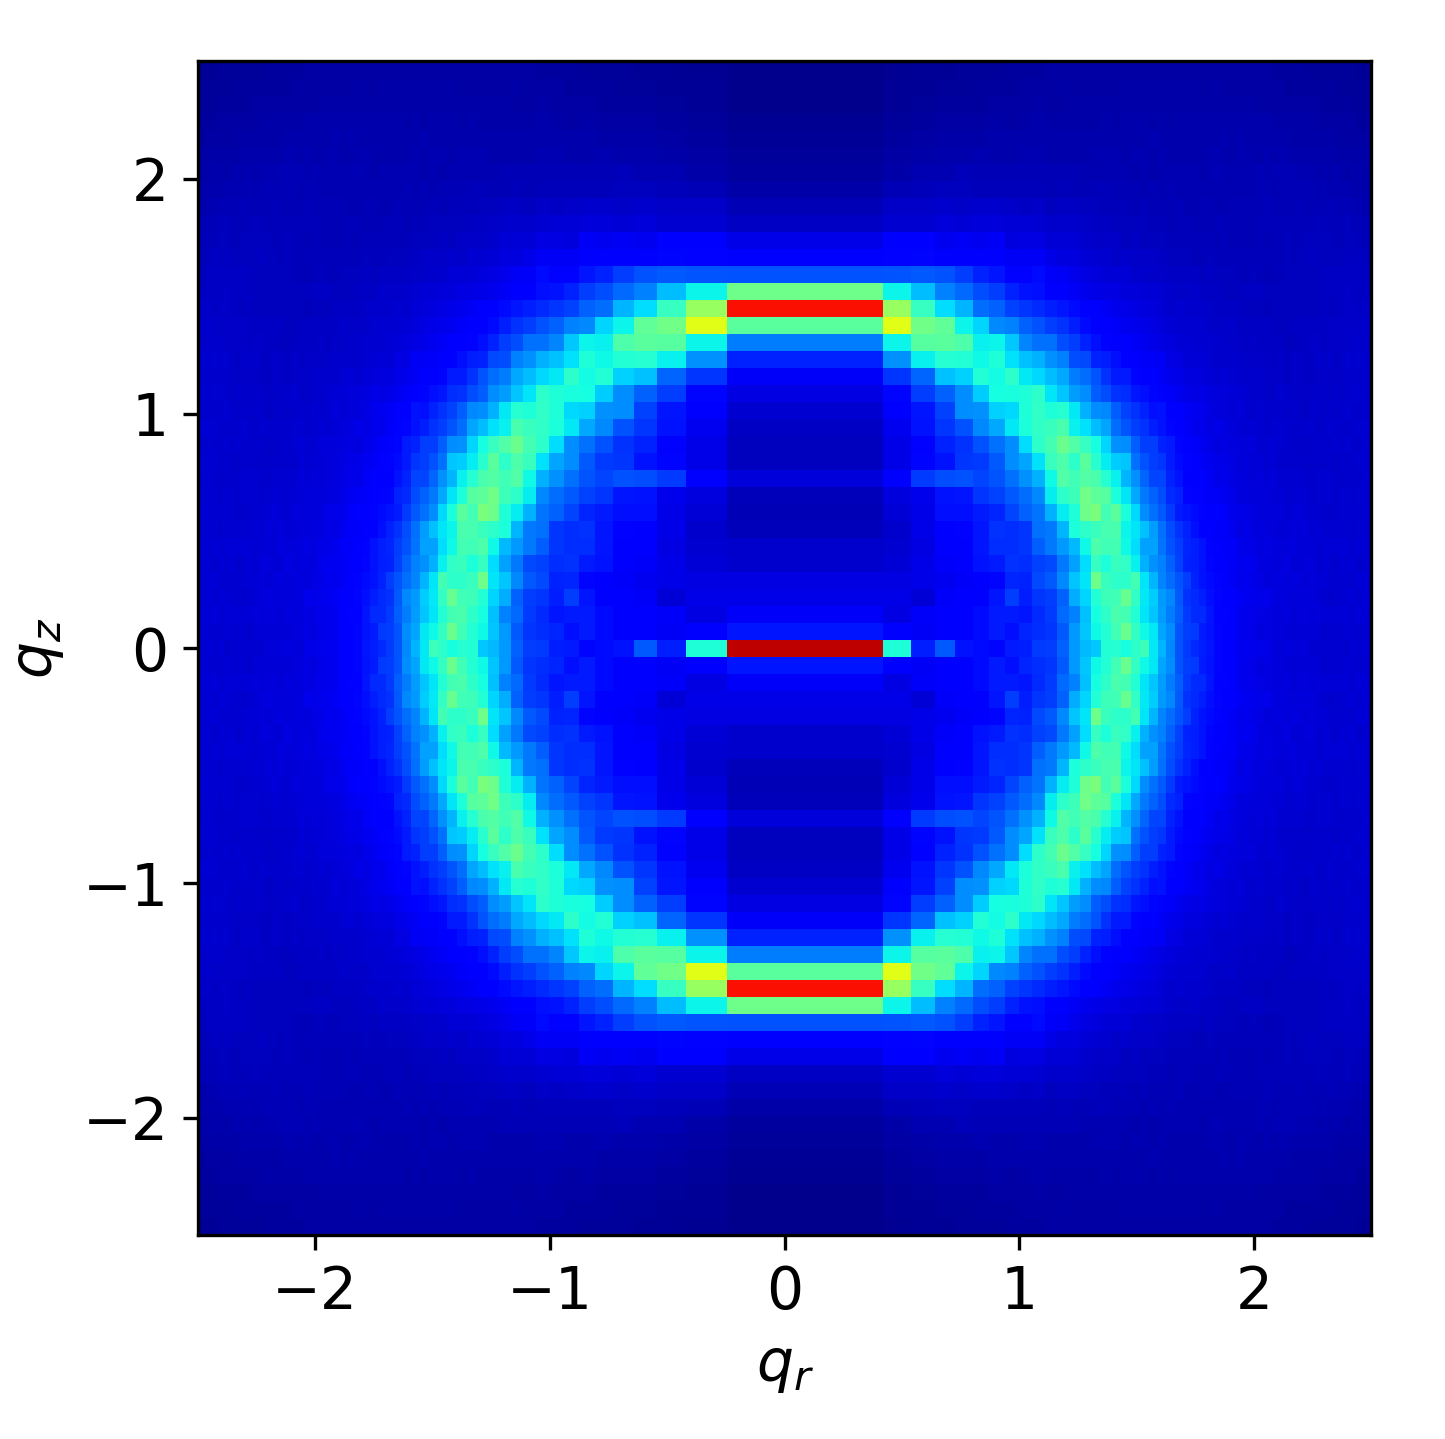
\includegraphics[width=1.1\linewidth,trim={1cm 0 1.3cm 0},clip]{offset_rzplot.png}
%        \caption{}~\label{fig:rz_offset}
%  \end{subfigure}
%  \begin{subfigure}{0.3\linewidth}
%        \centering
%%        \vspace{0.25em}
%        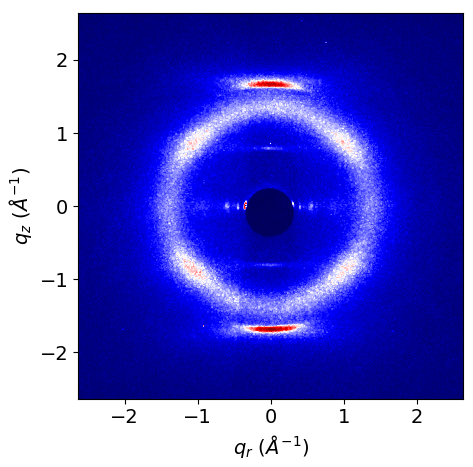
\includegraphics[scale=0.285]{WAXS_raw.png}
%        \caption{}~\label{fig:raw_waxs}
%  \end{subfigure}
%  \begin{subfigure}{0.3\linewidth}
%        \centering
%        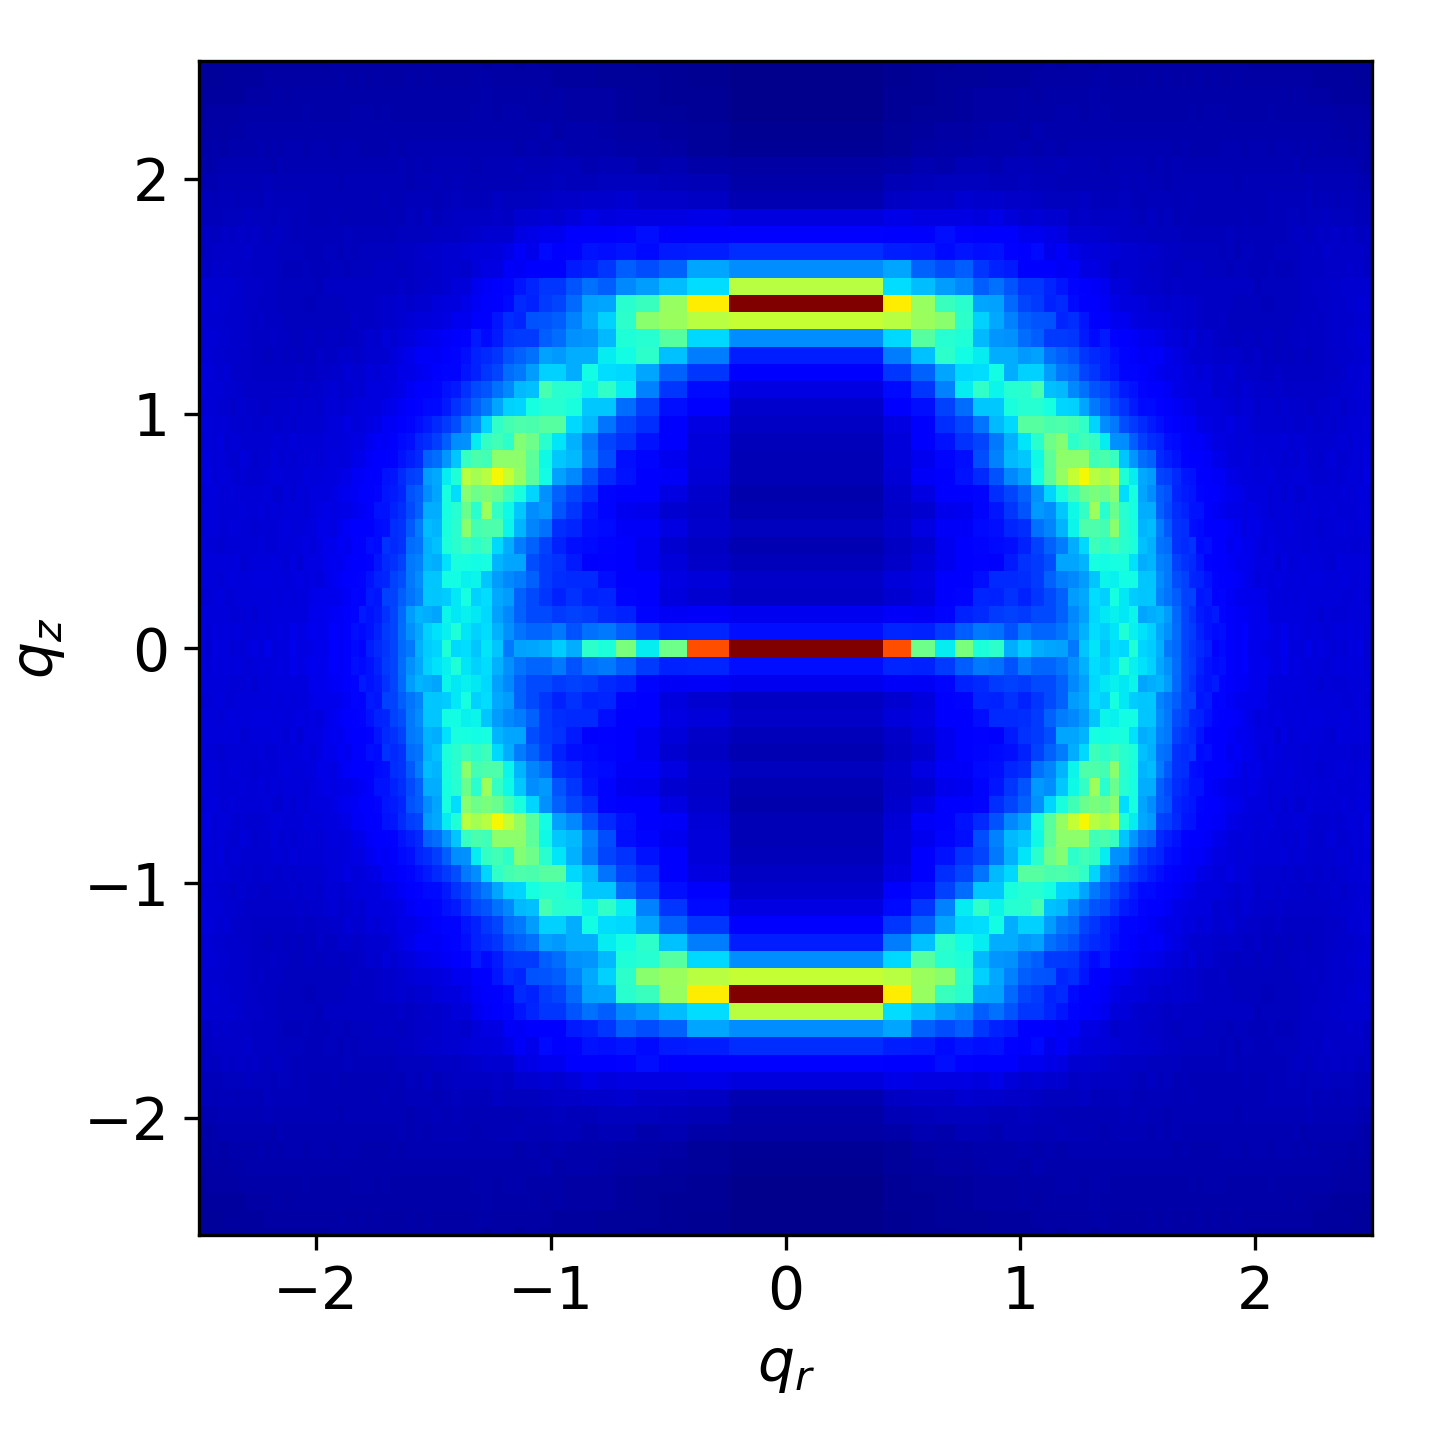
\includegraphics[width=1.1\linewidth,trim={1cm 0 1.3cm 0},clip]{layered_rzplot.png}
%        \caption{}~\label{fig:rz_layered}
%  \end{subfigure}
%  \begin{subfigure}{0.0544\linewidth}
%        \centering
%        \vspace{-4.00em}
%        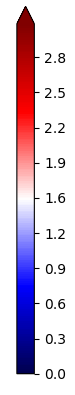
\includegraphics[width=\linewidth]{colorbar_seismic.png}
%  \end{subfigure}
%%MRS6: question: the SAXS region looks different between sandwiched and parallel displaced. Any thoughts why? We can discuss in person.  And seems like have to comment on the difference in intensity between Sandwich and parallel displaced in the pi-pi region.
%%MRS6: I wonder to what extent showing the reflections of tails removed would make it clearer pi-pi is really there.  Maybe in supporting info?
%%BJC2: Sure, I'll add that to supporting info
%  \caption{The simulated XRD pattern generated from the equilibrated trajectory
%	  of the parallel displaced configuration (a) exhibits all major reflections
%	  present in the experimental WAXS pattern (b). The simulated XRD pattern
%	  generated from the equilibrated trajectory in the sandwiched configuration (c) shows
%	  all major reflections except R-double.}
%  \label{fig:XRDsim}
%  \end{figure}

%  In both simulated diffraction patterns R-alkanes appears in the expected location. 
%  The location of R-pores is not well-defined in comparison to experiment. In order
%  to resolve those reflections it would be necessary to simulate a much larger system, 
%  but that is unnecessary since we can measure pore spacing manually as described 
%  earlier. R-$\pi$ and R

%  In both the parallel displaced and sandwiched configurations, we noted that
%  R-$\pi$ appears in a location which corresponds to a real space separation
%  larger than experiment. We attribute this discrepancy to GAFF's inability to
%  appropriately model the aromatic interactions which would be necessary to
%  achieve the correct $\pi$-$\pi$ stacking distance. 
%  %Systems have been modeled that exhibit the correct stacking distance, however
%  %they are typically made of planar molecules spanning a large area.
%  %BJC: I saw a paper like this a long time ago, but failed to save the citation and
%  % now I am having a hard time finding it again. 
%  The monomers in our model have bulky tails whose entropic contributions compete
%  with the $\pi$-$\pi$ stacking interaction energy. There have been efforts to
%  model systems that contain $\pi$ interactions in a classical mechanical context
%  using polarizable forcefields \cite{baker_polarizable_2015},
%  %MRS6: 
%  but they are significantly more computationally expensive to
%  reach the time scales required to equilibrate these systems at the present time.
%  %MRS6: not so relevant below.
%  %We could
%  %implement a polarizable force field, however it is likely not worth the extra
%  %computational cost. If our model proves to be inadequate when simulating
%  %transport, we will revisit our current choice of forcefield.  
%
%  In addition to R-$\pi$ being shifted to lower $\mathbf{q}$ values, a few
%  factors combine to make the simulated R-$\pi$ reflection visibly more intense
%  than in the experimental pattern. The simplest reason is that R-$\pi$ and
%  R-alkanes add together to boost the overall signal at intersecting values of
%  $\mathbf{q}$. In addition, we observe a much higher maximum intensity within
%  R-$\pi$. The maximum intensity within R-$\pi$ of the normalized experimental
%  pattern is 3.1, while the maximum intensity within R-$\pi$ of the normalized
%  parallel displaced simulated pattern is 32.9. 
%  %MRS2 10x is really big.  That seems hard to actually manage . . . I didn't realize it was that big. For some reason, I thought it was around 3x.  If it's that big, how come the 7.4 A reflection isn't big?  It's not clear to me how this is possible. Not clear how the angle averaging obscured this before?
%  %BJC2 From plots of raw structure factor, it doesn't seem like a normalization issue. It was probably obscured in the original angle averaging because it 
%  % was averaged with neighboring bins
%  While direct numerical
%  comparisons between simulation and experiment aren't necessarily precise due to
%  underlying assumptions, an order of magnitude difference suggests some
%  significance. We believe that we see such a high maximum for two reasons: (1)
%  We are simulating a perfectly aligned system so all X-rays reflected along the
%  pore axis would add constructively. The crystalline domains in the real system
%  are not perfectly aligned (See azimuthal distribution in Supporting
%  Information) which would lead to an overall decrease in the intensity of
%  R-$\pi$. (2) Our system is more ordered with high correlation between layers.
%  We will come back to this point further in ensuing discussions.
%
%  There is a grid-like pattern near $\mathbf{q}=0$ which appears because the
%  simulated system shows crystalline character. The grid features along nonzero
%  values of $q_z$ line up with reflections at $q_z=0$ which indicates positional
%  correlations between columns in the z-direction. This type of correlation is
%  expected for a crystalline material. 
%%MRS6: need some justification for why we are not totally surprised the system is crystalline.  But is is so crystalline in the x direction? The grid spacing is ``crystalline-ish'' in both x and z directions. . . we should talk. 
%If our system met the definition of a
%  columnar liquid crystalline system, we should observe only weak short-range
%  z-directional correlation within columns, with no correlation between
%  columns\cite{chaikin_principles_1995}. 
  
  \subsubsection{The location of R-alkanes}\label{section:ralkanes}

  We normalized the experimental and simulated diffraction patterns so that the
  average intensity within R-alkanes is equal to 1 because we believe that
  R-alkanes is the experimental feature most likely to be reproduced by our
  simulations.  We reach this conclusion because alkane parameters in GAFF and
  AMBER forcefields generally reproduce data well.~\cite{original_gaff_paper} 
  %MRS12: Citation is: https://doi.org/10.1002/jcc.20035  could also cite: https://pubs.acs.org/doi/pdf/10.1021/ct200731v

  %MRS12: below - say what appears close means?  radius of max is X vs Y.
  R-alkanes appears close to its expected location. In all cases, the maximum
  intensity of R-alkanes along the $q_r$ axis at $q_z$=0, which we use to
  estimate its location, appears at a $|\mathbf{q}|$ value that is, at most,
  3.5\% higher than higher than experiment. 
  %MRS12: different pass? Though need to specify WHAT the error is.  Can't be intensity, since that is what we are normalizing by, so is it LOCATION of the intensity?  Also, need to verify the statement is correct.  Could still good languange if the conclusion was that the binning error was similar in size to errors in the location R-alkane.
  %BJC12: I use the maximum intensity of R-alkanes along the q_r axis at qz=0 to determine its location.
  The error in the simulated diffraction patterns is less than the error due
  binning in each frequency direction, so was not further investigated. 
  %We expect that the exact location of R-alkanes will not be perfect in our simulations
  %since the simulated diffraction patterns are interpolated between a finite number of
  %bins in each frequency dimension. 
  %We can achieve higher resolution with a larger
  %system size, however we are satisfied with the packing distances shown by our simulations.
  %BJC11: I could integrate a 3D correlation function to get a better value.
  %MRS12: saying ``we are satisfied'' opens to claims that reviwers say ``well, I'm not''.  Pass at this above.

  \subsubsection{The location and intensity of R-pores}\label{section:rpores}
  
  R-pores is about 10 times more intense than experiment in all simulated
  systems. Some or all of this discrepancy may be a consequence of our
  normalization of the experimental 2D SAXS pattern, since the common peak
  between it and the 2D WAXS patterns is partially obscured by the beamstop in
  the WAXS. If our simulations do indeed predict an intensity of R-pores that is
  too high, we hypothesize that this is primarily due to the relatively perfect
  infinite hexagonal array of pores in the simulated systems. In the real system,
  periodicity of the hexagonal array is disrupted by misalignment of the
  crystalline domains and the pore-to-pore distances fluctuate more over long
  time scales. 
  % BJC11: Using simple systems, I can show that more highly fluctutating pore-to-pore
  % distances will decrease the intensity of R-pores. I don't think its worth getting
  % into in the main text. It's the same idea as how increased z-noise decreases the intensity of R-pi
  % BJC11: I also think that domain misalignment in the z-direction contributes. If you
  % imagine a hexagonal array of pores aligned along the z-axis, then rotate that axis
  % so it has an x and y component, then there will be constructive interference perpendicular
  % to that axis at non-zero qz values. That is why R-pores is arced. It's a different
  % type of broadening than R-pi - I think
  % BJC11: I don't think a deep dive into this is worth it. It's dependent on things
  % unrelated to the actual pore structure.
  % MRS12:  Agreed. Rephrased a bit.
  The agreement in intensity in R-pores obtained here is sufficient for this
  study because this intensity is primarily controlled by longer-range
  organization that cannot be captured by simulation of only 4 pores and because
  we are only concerned with the structure of the individual pores themselves. 
  
  The location of the leading peak of R-pores is directly related to the
  average distance between pores. However, there is substantial uncertainty in
  the exact location relative to the bin size resulting from the Fourier space
  transformation. We can instead measure the average distance between columns
  with more precision in real space (See Section~\ref{method:pore_spacing}). We
  showed that we achieve experimentally consistent pore spacings in our
  simulations in Section~\ref{section:mon_per_pore}. 

  \subsubsection{The origin of R-spots}\label{section:rspots}
  
  The intensity of R-spots is close to experiment when generated from any of
  our simulated systems. We measured the intensity of R-spots by radially integrating the simulated
  diffraction pattern between $1.4~\AA^{-1} < |\mathbf{q}| < 1.57~\AA^{-1}$
  (between 4 and 4.5 $\AA$ in real space) and then locating and recording the
  intensity of the appropriate peaks in the resulting distribution. Because the
  R-spots reflection is difficult to distinguish visually as it appears at the
  same $|\mathbf{q}|$ as R-alkanes, we calculate the intensity of R-spots by
  assuming that its $q_z$ location should be roughly in line with the
  experimental R-double, half the $q_z$ distance of R-$\pi$).

  %MRS12: here I'm going to break the rule of the thesis statement, since it reads strangely to have thesis, contradition, repeat thesis, there isn't any evidence. But it flows OK this way.   
  %R-spots is most likely a result of ordered packing of the monomer's alkyl tails. 
  Previous literature has attributed the R-spots reflection in this particular
  WAXS dataset as the result of tilted alkane chains~\cite{feng_scalable_2014}.
  We measured the tilt angle of the alkane chains of the 280K system by measuring
  the angle made by the vector extending from top to bottom of each tail with
  respect to the membrane plane. We found that it equilibrates to an average tilt
  angle of -2\degree~(Fig.~\ref{fig:tilt}), far from the 37\degree~tilt angle
  previously used to explain R-spots. Even when we placed position restraints on
  the monomers in a tilted initial configuration, monomers quickly reduced their
  tilt relative to the $xy$ plane to an angle statisically indistinguishable from
  zero. (See Section S-TBD). 
  %Similar lack of more than a statistically negligible
  %tilt occured when we performed the simulations with a number of other starting
  %configurations, obtaining similar results. 
  %MRS12: I know we discussed this earlier; there were a number of things that were done to verify this results was consistent, and I think that a rief summary would help. 
  %BJC12: It was primarily us trying to induce tilt by equilibrating with position restraints. I'm trying to think of what else we might have done. I changed the last sentence for now  

  In order to more clearly identify the structural reasons for R-spots, we
  equilibrated an ordered basin sandwiched configuration at 280K to moderately
  increase the order and therefore intensity.  Many force fields do not obtain
  the correct equilibrium structure at precisely the experimental temperature.
  Wang et al. highlighted the shortcoming of some of the most popular protein
  force field in predicting the temperature dependence of protein structural
  ensembles \cite{wang_building_2017}. It is therefore possible that   % page 12
  our membrane system, simulated at 300K, is under-structured in the tail region
  compared to the experimental structure at 300K. We found that lowering the
  temperature indeed better resolved R-spots (Figure~\ref{fig:sandwiched280K}),
  suggesting that our `effective' temperature might indeed be too high,
  understabilizing structure. 

%  The Evidence from the simulations strongly suggests that the R-spots signal
% is not a 
%  result of alkane chain tilt. 

  The evidence from simulations strongly suggest that the source of
  the R-spots reflection is packing of the tails in a hexagonal array.
  First, we demonstrate R-spots comes primarily from the tails, by
  removing all non-tail atoms from the trajectory and simulating the
  XRD diffraction pattern with the remaining atoms, which preserves
  R-spots (Figure~\ref{fig:tails_rzplot}).  Next, we plotted the center
  of masses of the first four tail atoms of all tails (Figure
  \ref{fig:centroids}). We measured the angle between each center of
  mass and its nearest neighbor center of masses with respect to the
  $xy$ plane of the membrane. We see distinct peaks in the
  distribution of these angles located ca. $-60\degree$, $0\degree$,
  and $60\degree$ which is consistent with a hexagonally packed
  configuration (Figure~\ref{fig:layered_tails}).  This ordering is
  primarily in the parts of the tail proximal to the heads, and dies
  off at the tail ends, where there is more space to fill causing them
  to pack nearly isotropically. See Section~S-\ref{S-section:tail_packing} for
  a more detailed explanation of the calculation and packing
  distributions generated from different sections of the tails.

  The peaks in the nearest neighbor angle distribution due to the hexagonal
  packing are consistent with the location of R-spots. The 2D Fourier transform
  of a simple hexagonal array constructed based on the peak angles in
  Figure~\ref{fig:layered_tails} shows reflections in the same locations as
  R-spots, in addition to vertical stacking reflections along the $q_z$ axis that
  would intersect with R-$\pi$ (Figure~\ref{fig:hexagonal_ft}). 

  \begin{figure}[!htb]
  \begin{subfigure}{0.32\linewidth}
  	\centering
  	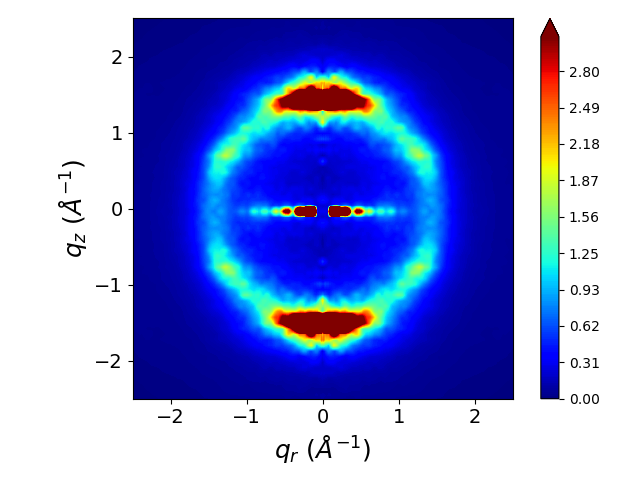
\includegraphics[width=\textwidth]{rzplot_layered_280K_jet.png}
  	\caption{}\label{fig:sandwiched280K}
  \end{subfigure}
  \begin{subfigure}{0.32\linewidth}
    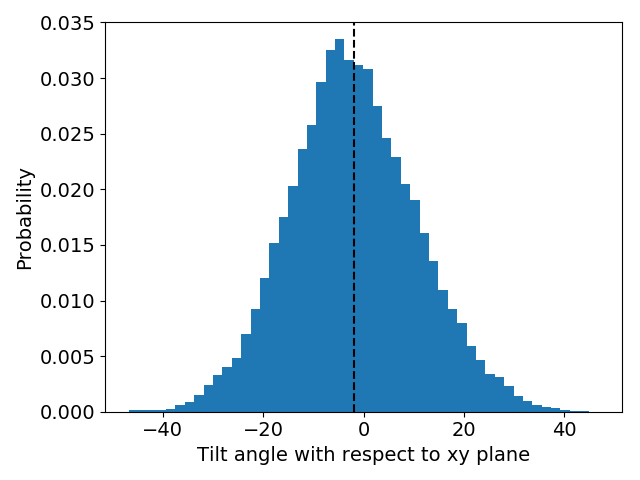
\includegraphics[width=\textwidth]{tilt_dist.png}
    \caption{}\label{fig:tilt}
  \end{subfigure}
  \begin{subfigure}{0.32\linewidth}
	\centering
	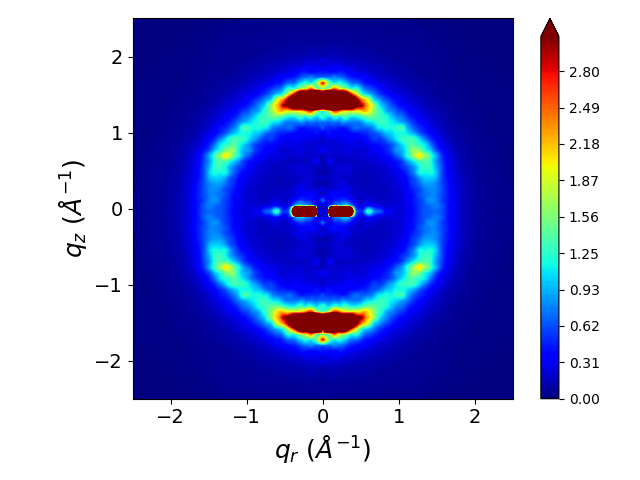
\includegraphics[width=\textwidth]{tails_rzplot_jet.png}
	\caption{}\label{fig:tails_rzplot}
  \end{subfigure}
  \begin{subfigure}[t]{0.32\linewidth}
    \centering
	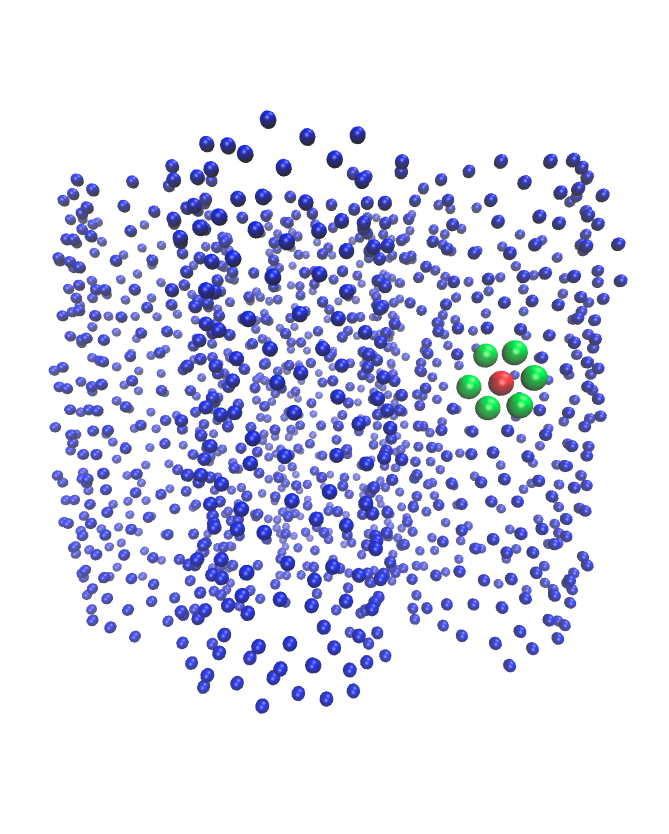
\includegraphics[scale=0.2]{centroids.png}
  \caption{}\label{fig:centroids}
  \end{subfigure}
  \begin{subfigure}[t]{0.32\linewidth}
        \centering
	        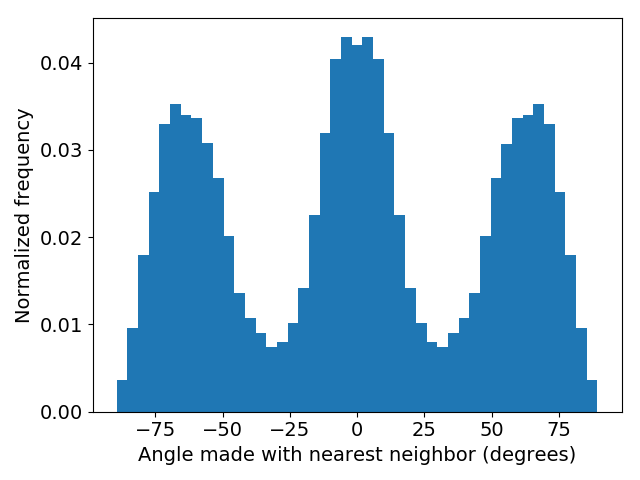
\includegraphics[width=\linewidth]{hexagonal_tail_packing.png}
	        \caption{}~\label{fig:layered_tails}
  \end{subfigure}
  \begin{subfigure}[t]{0.32\textwidth}
        	\centering
	        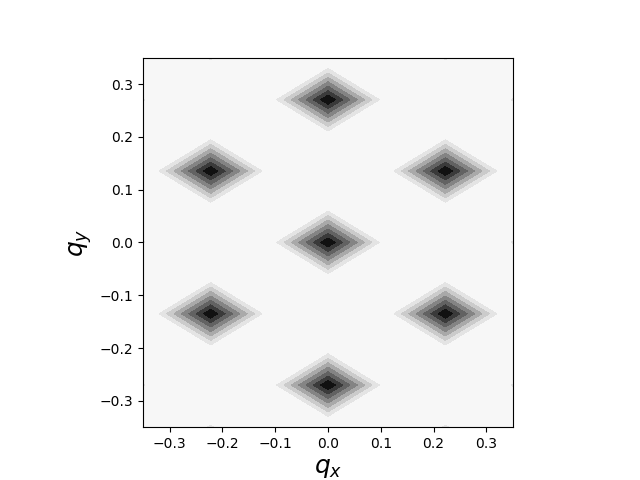
\includegraphics[width=\linewidth]{hexagonal_ft.png}  % generated from hexagonal_packing.py
	        \caption{}~\label{fig:hexagonal_ft}
  \end{subfigure}
  \caption{(a) R-spots increases in intensity when the temperature of the system is 
      lowered to 280K. (b) We measured the average angle made between each monomer 
      alkane tail and the membrane plane. The average tilt angle (dashed line) is 
      near -2\degree~which is far from the 37\degree~tilt angle previously used to
      explain R-spots. (c) To isolate the main cause of R-spots, we removed all atoms
      from the trajectory except for carbon atoms that constitute the tails. The
      simulated XRD pattern of the tails-only trajectory still shows R-spots. (d)
      Since the tails stay relatively flat, we plotted the center of mass of the first
      four carbon atoms of each tail originating from the head groups (for example,
      green colored centroids in the plot surround the red centroid in hexagonal fashion).
      Visually, the packing looks hexagonal. (e) We hypothesize
      that R-spots is the result of ordered tail packing. Defining
      the membrane plane to be 0\degree, we measured the angles between each center of 
      mass and its nearest neighbor center of masses for the equilibrated 
      sandwiched configuration simulated at 280K. Peaks appear in the distribution at 
      $-60\degree$, $0\degree$ and $60\degree$. (f) The Fourier transform of a hexagonally
      packed grid of points defined by the angles in (e) shows intensity at the same
      locations where we expect to see R-spots, as well as intensity along the $q_z$ axis
      where R-$\pi$ would appear.}~\label{fig:tail_packing}
  \end{figure}  

  \subsubsection{The position, shape and intensity of R-$\pi$}\label{section:rpi}

  The position, shape and intensity of R-$\pi$, generated from simulations at
%  300K, are qualitatively similar to experiment, but have significant
%  quantitative differences. 
% BJC12: I don't think I agree that they are qualitatively similar either. The
% simulated qr cross-sections are spikey and too low (which is qualitatively
% evident when you look at the simulated XRD patterns)
  300K have qualitative and quantitative differences from experiment.
  The reflections appear at lower $q_z$ values, they
  are more intense, and the shape of its cross-sections, especially in the $q_r$
  direction are different relative to the experimental system.  For comparison,
  see Figure~\ref{fig:rpi_exp_comparison} where we used cross-sections of the
  simulated XRD generated from the ordered parallel displaced configuration as an
  example. In this section, we explore the various contributions to these
  discrepancies, and use this information to speculate on what reasonable
  differences in the simulations could explain the discrepancies.
  
  \begin{figure}
  \centering
  \begin{subfigure}{0.45\textwidth}
  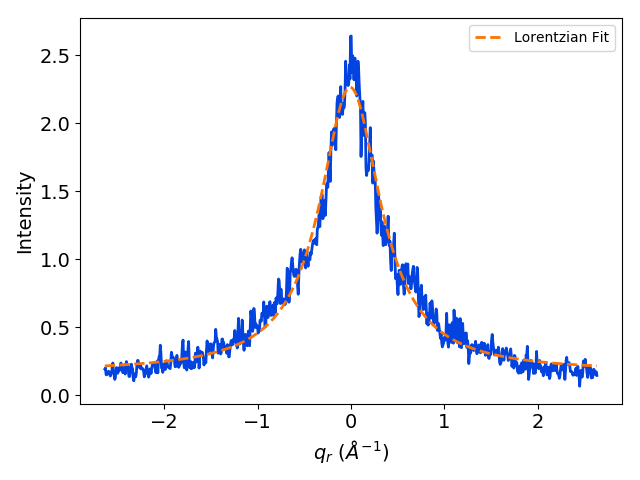
\includegraphics[width=\textwidth]{exp_rsection_fit.png}
  \caption{FWHM = 0.792 $\pm$ 0.009 $\AA^{-1}$}\label{fig:exp_rsection_fit}
  \end{subfigure}
  \begin{subfigure}{0.45\textwidth}
  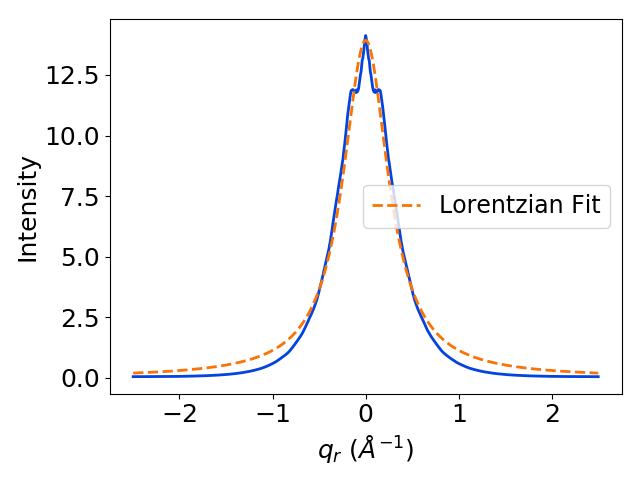
\includegraphics[width=\textwidth]{sim_rsection_fit.png}
  \caption{FWHM = 0.796 $\pm$ 0.011 $\AA^{-1}$}\label{fig:sim_rsection_fit}
  \end{subfigure}
  \begin{subfigure}{0.45\textwidth}
  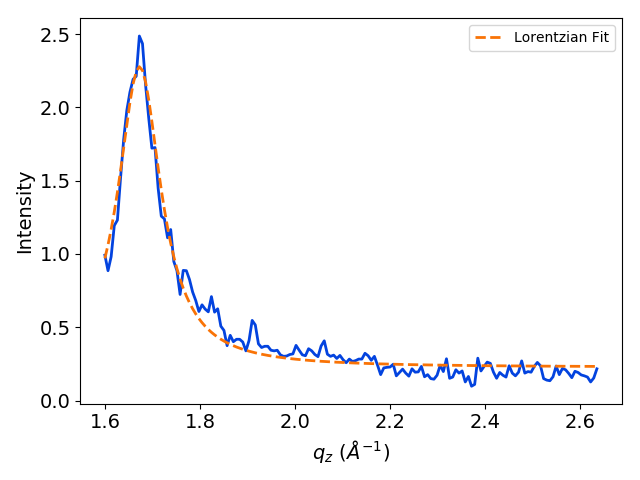
\includegraphics[width=\textwidth]{exp_zsection_fit.png}
  \caption{FWHM = 0.110 $\pm$ 0.003 $\AA^{-1}$}\label{fig:exp_zsection_fit}
  \end{subfigure}
  \begin{subfigure}{0.45\textwidth}
  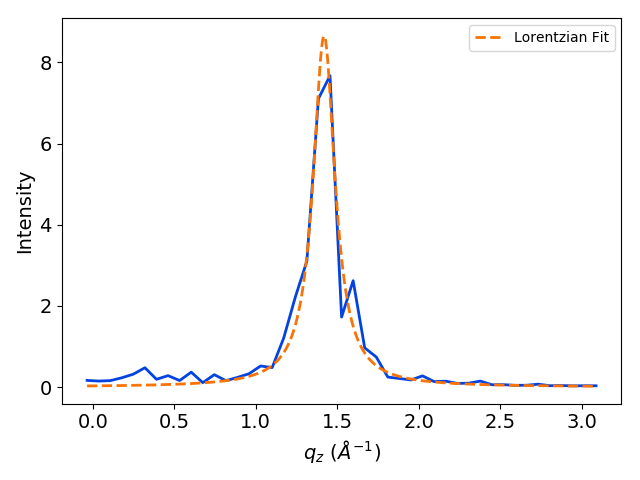
\includegraphics[width=\textwidth]{sim_zsection_fit.png}
  \caption{FWHM = 0.163 $\pm$ 0.011 $\AA^{-1}$}\label{fig:sim_zsection_fit}
  \end{subfigure}
  \caption{
  The maximum intensity of R-$\pi$ generated from simulations of the ordered
  parallel displaced configuration is 3 times larger than experiment. The $q_r$
  cross-section of R-$\pi$ ((a) and (b)) is qualitatively different between 
  experiment (a) and simulation (b). We fit Lorentzian profiles to each peak and
  the FWHM (full width at half maximum) of the simulated pattern agrees with experiment within error. However
  the fit to the simulated data is affected by the three sharp peaks which appear
  near $q_r$ = 0. The $q_z$ cross-sections of R-$\pi$ ((c) and (d)) are 
  qualitatively similar. Each fits a Lorentzian profile well, however the FWHM
  of the simulated cross-section (d) is 48\% larger than the experimental 
  cross-section. Additionally, the peak of the simulated $q_z$ cross-section is 
  located at a lower $q_z$ value than experiment.}\label{fig:rpi_exp_comparison}
  \end{figure}
  
%  The difference in intensity ranges from 3 times too high in the ordered parallel
%  displaced system to 15 times too high in the ordered sandwiched configuration 
%  (Table~\ref{table:relative_intensities_300K}).

  R-$\pi$ appears at a lower $q_z$ value in our simulations versus experiment because
  monomers in the simulated system stack further apart than those in the experimental
  system (Table~\ref{table:correlation_length}). We calculated $z$-direction pair distribution
  functions, $g(z)$, as described in Section~\ref{section:correlation_length}.
  %BJC11: Below is in methods but might be worth restating here? 
  %MRS12: no, OK here.
%  based on the center of mass of each monomer head group. In order
%  to calculate $g(z)$, we averaged all $z$-slices of the 3D pair distribution function, $g(x, y, z)$, 
%  (Equation~\ref{eqn:correlation}) within
%  2.1 \AA~of $g(0, 0, z)$. In this way we are measuring correlation between head 
%  groups within the same column. 
  The resulting distributions are generally characterized by decaying
  oscillatory behavior where the average distance between peaks corresponds to
  the average distance between stacked monomer head groups
  (Figure~\ref{fig:correlation}).  We calculated this equilibrated vertical
  stacking distance, $\mathit{d}_{equil}$, between monomers using
  Equation~\ref{eqn:decaying_sinusoid}. The distance between stacked monomers is
  greater than experiment by 0.5--0.9 \AA~across all cases, with disordered
  basins at the high part of that range and are on average 0.2 and 0.3 \AA~more
  distant. This behavior is
  not surprising since GAFF models atoms as point charges and  % BJC11: need reference %MRS12: just cite the GAFF paper.
  does not appropriately model the aromatic $\pi-\pi$ interactions, which would make
  it more energetically favorable for the monomers to stack closer together.  It
  is also possible that the tails prevent close stacking of monomer head groups
  and we do not achieve the timescales necessary for them to rearrange into a
  necessarily more tightly packed configuration. However, we equilibrated the
  system at 500 K then annealed it to 300 K in an attempt to coerce the tails into
  a more tightly packed configuration, however we saw no improvement in packing
  distance over our 300 K models. See section S-TBD for details.

  The system size, in the $z$-direction, does not significantly alter $g(z)$.
  In Figure~\ref{fig:correlation}, oscillations do not fully decay, so a taller
  system may be necessary to fully capture the correlation function. We therefore
  equilibrated a sandwiched system with twice as many monomers per column so that
  the system size doubled in the $z$-direction. The correlation length increases
  modestly from 4.5 $\pm$ 0.4 to 7.3 $\pm$ 1.2 \AA. However, visually, the
  correlation functions are nearly identical and oscillatory behavior persists
  throughout $g(z)$ in both cases (See
  Figure~S-\ref{S-fig:z_correlation_overlay}).

  The broadening of the $q_z$ cross-section of R-$\pi$ is related to
  $z$-directional correlation between scatters within monomer columns. The
  correlation length varies as the inverse of the full width at half maximum
  (FWHM) of the $q_z$ cross-section of R-$\pi$.  Using this technique, we
  calculated the correlation length of the experimental system to be 9.0 \AA. As
  scatterers become less correlated, we expect that R-$\pi$ will broaden.

  The correlation lengths of vertically stacked scatterers in our atomistic
  simulations are in reasonable agreement with experiment. Since it is not
  feasible for us to simulate membranes with much taller columns in order to
  obtain increased $q_z$ resolution of our simulated XRD patterns, and because
  the simulated peak shape is convoluted by the extremely intense maximum of
  R-$\pi$, we measured correlation length by fitting
  Equation~\ref{eqn:decaying_exponential} to the peaks of $g(z)$. The correlation
  length of the parallel displaced, ordered basin system shows the closest
  agreement with experiment (Table~\ref{table:correlation_length}). 
  %BJC11: below might confuse the reader
%  Note that its correlation length
%  ($L$ = 14.5 \AA) is larger than what we would expect by inverting the FWHM of the $q_z$
%  cross-section of R-$\pi$ shown in Figure~\ref{fig:sim_zsection_fit} ($L$ = 1 / 0.163 
%  = 6.1 \AA). The reason is likely a combination of artificial broadening caused by the
%  overlap of R-alkanes and R-$\pi$ as well as uncertainty in the fit due to low simulated
%  XRD resolution.
  We could not extract a reliable correlation length from the disordered
  parallel displaced configuration since the peaks do not show clear patterns
  that can easily be fit to an exponential decay. The correlation length of both
  sandwiched systems are relatively low because the height of the first peak of
  $g(z)$ is so high. 
  
  %BJC11: trying to figure out how to communicate distance correlation
  % wikipedia's explanation of distance correlation makes it seem like we are using it right:https://en.wikipedia.org/wiki/Distance_correlation
  % could say "distance covariance"
  Overall, we believe our simulations exhibit a realistic amount of distance
  correlation in the direction parallel to the pore axis between head groups
  within each column. The difference in the FWHM of the $q_z$ cross-section of
  R-$\pi$ between experiment and simulation is less than one bin size
  (Figures~\ref{fig:exp_zsection_fit} and ~\ref{fig:sim_zsection_fit}). The more
  signficant difference between the two cross-sections is their maximum intensity
  which we study in more detail below.
  
  \begin{figure}[!htb]
  \centering
  \begin{subfigure}{0.45\textwidth}
  \centering
  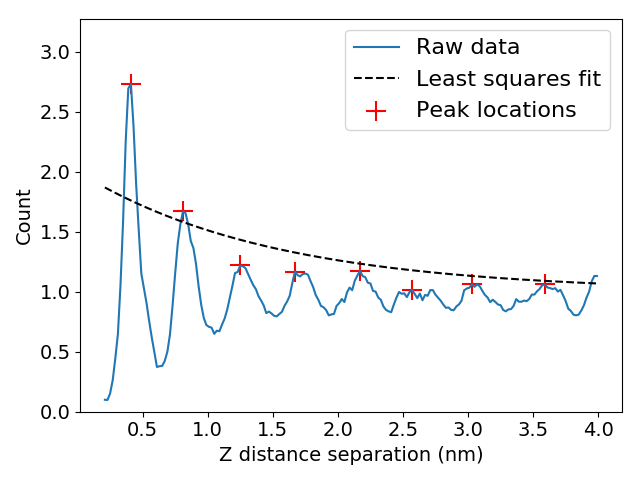
\includegraphics[width=\textwidth]{z_correlation_sandwich.png}
  \caption{Sandwiched, Ordered Basin}\label{fig:z_correlation_sandwich}
  \end{subfigure}  
  \begin{subfigure}{0.45\textwidth}
  \centering
  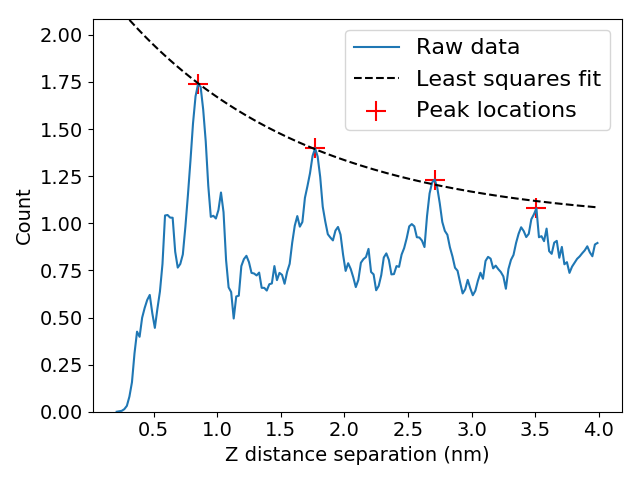
\includegraphics[width=\textwidth]{z_correlation_offset.png}
  \caption{Parallel Displaced, Ordered Basin}\label{fig:z_correlation_offset}
  \end{subfigure}  
  \begin{subfigure}{0.45\textwidth}
  \centering
  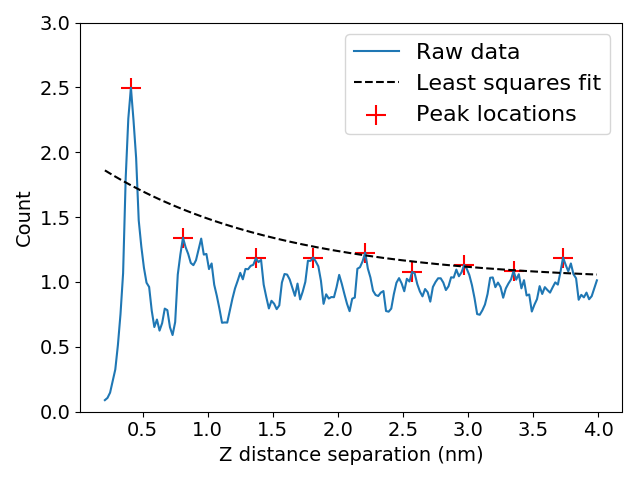
\includegraphics[width=\textwidth]{z_correlation_sandwich_disordered.png}
  \caption{Sandwiched, Disordered Basin}\label{fig:z_correlation_sandwich_disordered}
  \end{subfigure}  
  \begin{subfigure}{0.45\textwidth}
  \centering
  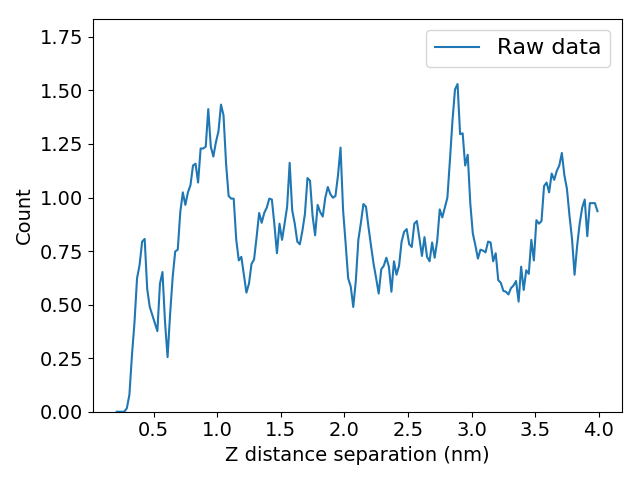
\includegraphics[width=\textwidth]{z_correlation_offset_disordered.png}
  \caption{Parallel Displaced, Disordered Basin}\label{fig:z_correlation_offset_disordered}
  \end{subfigure}  
  %MRS10: should say something here about whether this is consistent or not with experiement (and why/why not)
  %MRS10: maybe include correlation lengths as well calculated from these, and compare to experiment?  I know it's in the table as well, but seems missing here.  1D correlation functions are given, but not how that data proves central points.
  \caption{1D correlation functions of the center of masses of aromatic head
	  groups, $g(z)$, show decaying oscillatory behavior and have consistent correlation lengths with experiment. We calculated the
	  correlation length by fitting a decaying exponential function
	  (Equation~\ref{eqn:decaying_exponential}) to the peaks of $g(z)$. The
	  correlation length is longer for ordered basin systems
	  (Table~\ref{table:correlation_length}). We did not attempt to calculate the
	  correlation length for (d) because there are no clear peaks. We assume that its
	  correlation length is less than the vertical distance between monomers.}\label{fig:correlation}
  \end{figure}  
  
  \begin{table}[h]
  \centering
  \begin{tabular}{cccc}
  \toprule
  System             & $\mathit{d}$ (\AA) & $\mathit{d}_{equil}$ (\AA) & Correlation Length (\AA) \\
  \midrule
  Sandwiched         & 3.7                &    4.27 $\pm$ 0.03         & 4.2 $\pm$ 0.8            \\
  Parallel Displaced & 3.7                &    4.33 $\pm$ 0.04         & 14.5 $\pm$ 1.3           \\ 
  Sandwiched         & 5.0                &    4.48 $\pm$ 0.07         & 3.2 $\pm$ 0.9            \\
  Parallel Displaced & 5.0                &    4.60 $\pm$ 0.08         & $<$ $d_{equil}$ \\ 
  Experiment         & --                 &    3.70                    & 10 $\pm$ 1               \\
  \bottomrule
  \end{tabular}
  \caption{The correlation length is larger for systems in the ordered basin. The equilibrated vertical
  stacking distance, $\mathit{d}_{equil}$, is also smaller.}
  \label{table:correlation_length}
  \end{table}

  In addition to the maximum intensity of R-$\pi$ being too high, the shape
  of its $q_r$ cross-section in the simulated XRD is qualitatively different
  from experiment (Figures~\ref{fig:exp_rsection_fit}
  and~\ref{fig:sim_rsection_fit}). We attempted to fit a Lorentzian profile to 
  the $q_r$ cross-section and although the FWHM agrees with experiment within
  error, the fit is not optimal due to the three sharp peaks that appear near
  $q_r$ = 0. 
  
  An exact quantitative comparison between the intensity and FWHM of the
  experimental and simulated cross-sections of R-$\pi$ is not feasible for
  several reasons. Experimental peaks broaden due to effects that we can not
  easily simulate such as finite size crystalline domains and instrumental % reference needed
  resolution.  In our simulated XRD patterns, the system size imposes limitations
  on the resolution, which makes it difficult to reliably fit peaks. This is
  especially problematic when comparing the FWHM of the $q_z$ cross-section of
  R-$\pi$, where the experimental FWHM (0.11 $\AA^{-1}$) is similar to the bin
  size in the $q_z$ direction (ca. 0.07 $\AA^{-1}$).  Additionally, we model each
  atom with a Gaussian sphere of electron density, which is a simplification.
  However, we can explore reasons for which differences in the simulation
  structure could change the peak shapes and intensities to be in better
  agreement with experiment.

% BJC9: old version of above paragraph
%  The full width at half maximums (FWHM) of the $q_r$ and $q_z$ cross-sections
%  of R-$\pi$ are broader than experiment (Figure~\ref{fig:rpi_exp_comparison}).
%  The FWHM of the $q_z$ cross-section is 76\% larger than experiment and the
%  $q_r$ cross-section FWHM is 21\% larger than experiment. Note that the
%  experimental data is best fit with a Lorentzian function while the simulated
%  patterns are best fit using a Gaussian function. The simulated spectra do not
%  incorporate the effects of finite domain sizes, pressure broadening and
%  instrumental broadening which would alter the peak shape. In the absence of
%  these and other peak broadening effects, the experimental peak would actually
%  be narrower, further increasing the discrepancy with simulation.

% BJC11: paragraph seems unnecessary
%  We have identified a number of potential ways that simulation conditions,
%  forcefield and initial configurations could affect the intensity and shape of
%  R-$\pi$, and we assessed each using a simplified model of the pores. Our simplified model 
%  represents each monomer head group as single point scatterers and places them in either
%  a parallel displaced or sandwiched configuration. We chose to explore the 
%  influence of thermal noise in each dimension, the effect of $z$-direction 
%  distance correlations between scatterers within columns, as well as correlation
%  between columns since these are the variables we believe have the largest 
%  influence on peak shape and intensity.
   
  We studied the shape and intensity of R-$\pi$ by setting up simplified
  systems where we represent monomer head groups as point scatterers, as
  described in Section~\ref{method:simple_systems}. The amount of quenched and
  thermal disorder present in the atomistic system, which we applied to the
  simplified systems, are given in Table~\ref{table:quenched_disorder}. The
  quenched disorder, the deviation of monomers from idealized symmetric
  configurations, is several times greater than thermal disorder, the 
  deviations of the monomers from their average positions during the 
  production simulations. We hypothesize that, experimentally, the quenched disorder is the 
  same as thermal disorder, but we cannot reach the necssary transition
  timescales to fully thermalize in these simulations.  
  %MRS12: when reworking the first part of the simulation, our hypothesis for the REASONS behind the quenched disorder will ahave to be addressed. The two options are 1) the quenched disorder is just thermal disorder whose transition timescales we can't reach, and 2) the system if simulated for miliseconds/seconds would still be glassy. It PROBABLY should go before here, when it's first described.
  %BJC12: I first describe in methods, which seems the wrong place to put that hypothesis, so I tacked it on here.
  
  \begin{table}[h]
  \centering
  \begin{tabular}{c|ccc|ccc}
  \toprule
   		                        &           \multicolumn{3}{c}{Thermal Disorder}             &             \multicolumn{3}{c}{Quenched Disorder}               \\
  \midrule
  System                        & $\sigma_x$ ($\AA$) & $\sigma_y$ (rad) & $\sigma_z$ ($\AA$) & $\sigma_z$ ($\AA$) & $\sigma_\theta$ (rad) & $\sigma_r$ ($\AA$) \\
  \midrule
  Ordered Sandwiched            &         0.31       &       0.33       &        0.34        &        1.48        &     0.43              &     2.30           \\
  Ordered Parallel Displaced    &         0.51       &       0.52       &        0.30        &        1.45        &     0.43              &     2.28           \\ 
  Disordered Sandwiched         &         0.41       &       0.57       &        0.32        &        1.58        &     0.43              &     2.93           \\
  Disordered Parallel Displaced &         0.39       &       0.31       &        0.33        &        1.65        &     0.43              &     2.63           \\
  \bottomrule
  \end{tabular}
  \caption{Deviation of the positions of the center of mass of head groups from their average
  positions (thermal disorder) as well as their idealized positions (quenched disorder) to use 
  as simulated disorder into our model system.}
  \label{table:quenched_disorder} 
  \end{table}

  %MRS10: somewhere in here, we need to address whether thermal and quenched disorder are 
  % the same experimentally. If not the same, then it's glassy, if they are the same, then 
  % we are making the assumption that the the timescales of motion of that noice are > 1 microsecond but < 1 second.  
  %BJC11: most of this section moved to methods.
%  We can study the shape and intensity of R-$\pi$ using a simplified baseline model
%  which has the same amount of disorder present in our atomistic simulations. For these
%  models, we represent each monomer as single point scatterers located at the center of mass of
%  each monomer head group, and place them in a configuration spatially similar to those
%  seen in our simulations. We made them 4 times taller in the $z$-direction in order to access
%  higher $q_z$ resolution. When placing points, there are two sources of disorder to consider: 
%  thermal motion of atoms and quenched disorder which is created by rapid structural 
%  rearrangement during early equilibration and is largely locked into place for the remainder
%  of the simulation. We measured thermal disorder by calculating the standard deviation of 
%  the distribution of head group center of mass positions from their average positions. We 
%  measured quenched disorder by calculating the standard deviation of the distribution of head
%  group center of masses from their idealized average positions. In the $z$-direction, we
%  measured the deviation of the head group center of masses from an equally spaced column
%  of head groups. In the $xy$ plane, we calculated the standard deviation in radial position
%  from the pore center and the angular deviation from equally spaced points surrounding 
%  the pore center. This method for calculating quenched order inherently includes thermal 
%  disorder. The values measured for each system and type of disorder are given
%  in Table~\ref{table:quenched_disorder}. The magnitude of quenched disorder is greater than
%  thermal disorder.
  
  %BJC11: moved a variation of this to methods
%  To avoid any dependence on initial configuration, we calculated the average R-$\pi$
%  profile using simple system trajectories of 1000 independent configurations. We
%  determined the amount of disorder to add to each independent configuration using
%  the values for quenched disorder given in Table~\ref{table:quenched_disorder}. 

  %MRS10: this is more of a methodological thesis than is ideal. Can you make it more about what we are learning, or at least what was done and the reasoning?  
%  The expected maximum intensity of R-$\pi$ can be calculated from a single
%  trajectory of uncorrelated configurations rather than from the average of 
%  multiple trajectories of correlated frames. Theoretically, in order to
%  mimic the simulated system, we should build an initial configuration which 
%  has the same amount of quenched disorder as our simulations and then create
%  a trajectory to which we add thermal noise to each subsequent frame. In this
%  scenario, the positions of each scatterer will not change in a way that 
%  significantly affects the intensity of R-$\pi$ since most of its character 
%  is defined by the far more disordered initial configuration. To uncover the
%  expected intensity of R-$\pi$, we would need to average over many such 
%  trajectories. To bypass this expensive calculation, we instead calculate the
%  R-$\pi$ intensity from a trajectory consisting of many independent initial 
%  configurations. This simulates the long time scales over which we expect 
%  columns to sample many configurational states. %We use the latter method 
%  %for the remainder of this section since we can extract the trends we 
%  %need using a single trajectory at a fraction of the computational cost.

% BJC11: I eliminated this figure and the discussion of distance correlation between
% scatterers since the only real issue with the qz cross-section is the intensity. 
% I explain how we create correlated distances in the methods. We weren't really 
% showing anything new since correlation length equal 1 / FWHM_qz
%  \begin{figure}[!htb]
%  \centering
%  \begin{subfigure}{0.3\textwidth}
%  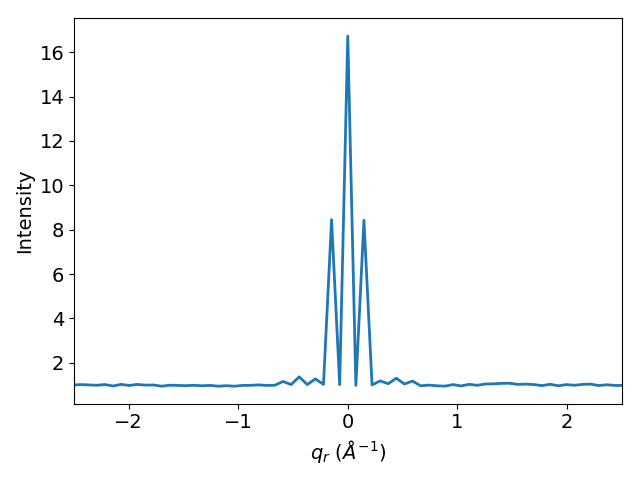
\includegraphics[width=\textwidth]{sf_qy_nocorrelation.png}
%  \caption{}\label{fig:sf_qy_nocorrelation}
%  \end{subfigure}
%  \begin{subfigure}{0.3\textwidth}
%  \includegraphics[width=\textwidth]{sf_qy_correlation.png}
%  \caption{}\label{fig:sf_qy_correlation}
%  \end{subfigure} 
%  \begin{subfigure}{0.3\textwidth}
%  \includegraphics[width=\textwidth]{sf_qz_correlation.png}
%  \caption{}\label{fig:sf_qz_correlation}
%  \end{subfigure}   
%  \caption{We generated X-ray diffraction patterns for simplified systems consisting of 
%  points meant to represent monomer head groups. We added a similar amount of noise to 
%  that seen in our simulations. (a) We added Gaussian noise to each particle in the $z$, 
%  $\theta$ and $r$ directions. The $q_y$ cross-section of R-$\pi$ contains three sharp
%  peaks. (b) When we correlate the distance between points within each column, the 
%  intensity of R-$\pi$ increases but the sharp peaks remain with the same ratio of
%  intensity between the center and outer peaks. (c) Correlation of the distance between
%  scatterers in the $z$-direction causes R-$\pi$ to broaden in the $q_z$ direction.}\label{fig:sf_correlation}
%  \end{figure}

%  The $q_r$ and $q_z$ profiles of R-$\pi$ generated from a simplified parallel displaced trajectory
%  where we represented monomer head groups with point scatterers exhibits sharp peaks with
%  no breadth. Figure~\ref{fig:sf_qy_nocorrelation} and~\ref{fig:sf_qz_correlation} shows
%  the $q_y$ and $q_z$ cross-sections of R-$\pi$ generated by simulating the structure 
%  factor of the trajectory. The distance between peaks in the $q_y$ cross-section is 
%  equivalent to the distance between pores in real space.
  
  % BJC11: probably unnecessary discussion. Could add to supplemental.
%  Correlation between scatterers increase the intensity of R-$\pi$ and broadens
%  its $q_z$ cross-section. In the simplified system described above, we added
%  Gaussian noise to the mean positions of an equally spaced column of points. 
%  This ignores any interaction head groups might have with each other. To remedy
%  this, we placed points in the $z$-direction by drawing random samples from a
%  multivariate normal distribution defined by the mean positions of an equally
%  spaced column of points. We gave the distribution at each point along the column
%  the same standard deviation, $\sigma_z$, shown in Table~\ref{table:quenched_disorder}.
%  We defined a covariance matrix such that the covariance, $v$, of the distance, 
%  $d$, between scatterers decays exponentially from $v$ according to the equation
%  $ve^{-d/L}$, where $L$ is the correlation length. We simulated the structure
%  factor of a simple system built as described above with a correlation length of
%  30 $\AA$. We chose 30 $\AA$ in order to exaggerate the effect of correlation
%  length for visual purposes. Subsequent structure factor calculations are all
%  done with a correlation length of 9 $\AA$. The shape of the $q_y$ cross-section
%  (Figure~\ref{fig:sf_qy_correlation}) remains the same while the the $q_z$
%  cross-section (Figure~\ref{fig:sf_qz_correlation}) broadens, as seen in
%  experiment. Additionally, there is a near 20\% increase in the maximum
%  intensity of R-$\pi$ when the distances between scatterers are correlated.

  %BJC8: Can show correlation effect on intensity in supporting info

% BJC9: omitted because these are not strong points
%  The peak height
%  indicates the degree of local ordering and influences the intensity of R-$\pi$.
%  If vertically adjacent sandwiched head groups were less ordered, which might be
%  achieved with much longer simulations, then the leading peak intensity should
%  decrease and the correlation length would increase. We expect that the leading
%  peak would only get more intense if monomers stacked 3.7 \AA~apart. Conversely,
%  parallel displaced head groups are not as confined by their vertically adjacent
%  neighbors. This z-direction translational freedom may still be feasible if
%  monomers stack 3.7 \AA~apart in a parallel displaced configuration, meaning the
%  system would maintain a correlation length and R-$\pi$ intensity in relative
%  agreement with experiment.
  
  Increasing thermal noise in the $z$-direction will reduce the intensity
  of R-$\pi$, however the $q_r$ profile remains unchanged. When we increase the
  thermal noise of the simplified parallel displaced system in the $z$-direction by
  12\% and 27\%, we see a 3 and 15-fold decrease in the maximum intensity of 
  R-$\pi$ respectively (Figure~\ref{fig:znoise}). Despite the decrease in 
  intensity, the 3 cross-sections have the same shape 
  (Figure~\ref{fig:rpi_xsection_vs_zsigma}), whose sharp Bragg-like peaks are
  not consistent with experiment. 
  
  \begin{figure}[!htb]
  \centering
  \begin{subfigure}{0.45\textwidth}
  \includegraphics[width=\textwidth]{intensity_vs_zsigma.png}
  \caption{}\label{fig:intensity_vs_zsigma}
  \end{subfigure}
  \begin{subfigure}{0.45\textwidth}
  \includegraphics[width=\textwidth]{rpi_xsection_vs_zsigma.png}
  \caption{}\label{fig:rpi_xsection_vs_zsigma}
  \end{subfigure}
  \caption{We can decrease the maximum intensity of R-$\pi$ by increasing
  thermal noise in the $z$-direction, however the $q_r$ cross-section profile does
  not change. (a) The intensity of R-$\pi$ drops precipitously as we increase
  $\sigma_z$. We can decrease the intensity of R-$\pi$, relative to the
  background intensity, relative to systems with simulation levels of disorder (blue)
  %as seen in simulation (blue) 
  by a factor of 3 when we
  increase $\sigma_z$ by 12\% (green) and by a factor of 15 when we increase
  $\sigma_z$ by 27\% (red). (b) Although the maximum intensity of R-$\pi$
  decreases with increasing $\sigma_z$, the peak shape remains the same.}\label{fig:znoise}
  \end{figure}
  
  However, when we allow monomer columns to move independently in the
  $z$-direction, the intensity of R-$\pi$ drops and the $q_r$ cross-section of
  the simulated diffraction patterns smooths out. We can demostrate this by
  creating a simplified sandwiched configuration (simplified in the same way as
  described above), 
  %simple systems 
  %MRS10: simple systems is not very exact. Point scatters that represent the head groups?
  %BJC11: It feels redundant and wordy saying the above rather than simple systems.
  with varying amounts of statistical correlation between columns. In the low
  limit, the center of mass of columns are situated at the same $z$-coordinate.
  We allow increasing independence of columns by randomly shifting each column in
  the $z$-direction according to a uniform distribution bounded by (0, $f \times
  \mathit{d}_{equil}$) where $f$ ranges between 0 and 1. We limit this discussion
  to the sandwiched configuration since it is not feasible for columns in the
  parallel displaced configuration, as we have set them up, to move past each
  other. When $f = 1$, the columns move independently and the $q_r$ cross-section
  smooths out completely (Figure~\ref{fig:column_displacement}). Any amount of
  dependence results in some presence of independent sharp peaks, though
  significantly attenuated at $f$ nearer 1. The intensity of R-$\pi$ also
  decreases with increasing column independence. We see an 8-fold decrease in the
  intensity of R-$\pi$ when $f=1$ versus when $f=0$ for our simplified model
  systems.
  %MRS12: somewhere will have to talk about stability and relative free energy of the more disordered initial configurations.
  %MRS12: we MIGHT have to look at more disordered initial configurations. I think this can likely be done with just equilibration, where we see how different the quenched disorder when starting from an ensemble of structures, and putting off actually calculating scattring from a large number of simulations. 
  \begin{figure}
  \centering
  \begin{subfigure}{0.3\textwidth}
  \includegraphics[width=\textwidth]{sf_qy_sr0.png}
  \caption{$f$ = 0}\label{fig:sf_qy_sr0}
  \end{subfigure}
  \begin{subfigure}{0.3\textwidth}
  \includegraphics[width=\textwidth]{sf_qy_sr75.png}
  \caption{$f$ = 0.75}\label{fig:sf_qy_sr75}
  \end{subfigure}
  \begin{subfigure}{0.3\textwidth}
  \includegraphics[width=\textwidth]{sf_qy_sr100.png}
  \caption{$f$ = 1}\label{fig:sf_qy_sr100}
  \end{subfigure}
  \caption{As we increase column independence using the $f$ parameter, the
	  intensity of R-$\pi$ decreases and the $q_r$ cross-section of the simulated
	  diffraction pattern becomes more smooth.  (a) When we place all columns at the
	  same reference $z$ coordinate, $f$ = 0, the intensity of R-$\pi$ is 18.3 and is
	  characterized by sharp Bragg-like peaks. (b) When columns have a moderate
	  amount of independence, $f$ = 0.75, the intensity of R-$\pi$ decreases 5-fold
	  to 3.7. The edges of the peak are beginning to smooth out, but sharp peaks
	  still exist. (c) When columns are completely independent, $f$ = 1, the
	  intensity of R-$\pi$ decreases 8-fold to 2.3 and the cross-section is
          relatively smooth.}\label{fig:column_displacement}
  \end{figure}

  It therefore seems likely that the discrepancy between the intensity of
  R-$\pi$ generated from our simulations versus experiment is primarily due to
  highly correlated columns in our initial configurations, likely due to the
  highly symmetric starting configuration. If the columns were uncorrelated,
  $g(z)$ of the ordered sandwiched system would very closely resemble
  Figure~\ref{fig:z_correlation_sandwich} when we average all $z$-slices of the
  3D correlation function. When we include all $z$-slices in $g(z)$ for our
  system, the function shows oscillatory behavior and the correlation length
  nearly triples to 12.4 $\pm$ 0.7 \AA. (Figure~\ref{fig:z_correlation_fullbox}).
  Since all columns in our initial configuration are started at the same
  $z$-coordinate, $g(z)$ on average exhibits correlation of head groups with
  other head groups within the same column, with head groups in other columns
  within the same pore, and with head groups in different pores.

  %BJC9: Note that the magnitude of the correlation function is much lower than 
  % in figure 10a. That's because many of the z-slices are zero when you include
  % all of them.
  \begin{figure}
  \centering
  \includegraphics[width=0.5\textwidth]{z_correlation_fullbox.png}
  \caption{When we average all $z$-slices of the 3D correlation function, the 
  correlation length of the ordered sandwich configuration nearly triples.}\label{fig:z_correlation_fullbox}
  \end{figure}
 
  Increasing thermal noise in the $xy$ plane causes the FWHM of the $q_r$
  cross-section of R-$\pi$ to, somewhat counterintuitively, decrease. Using a 
  system with uncorrelated columns, we modified the disorder in both the $r$ and
  $\theta$ directions by multiplying their values by a factor of 0.5 and 2 
  (Figure~\ref{fig:qy_fwhm}). When we cut the noise in half, the FWHM increases
  by 88\%. When we double the noise, the FWHM decreases by 51\%. As we have fit
  the data in Figure~\ref{fig:sim_rsection_fit}, the FWHM of R-$\pi$ agrees
  well with experiment, meaning the quenched configuration contains about the
  right amount of disorder on the $xy$ plane. However, the relatively low quality
  of the fit implies that the FWHM may be incorrect, and that the radial ordering
  of the head groups may benefit from further optimization.
  %MRS12: is there a structral 
  %implicatiob to the above?  It should be given explicitly so readers see where it fits in the story .
  % It could be that there is no real structural implication, which is fine, as long as its explicitly stated. 
  %is q_r cross-section right in experiment?  Does this explain differences our simulations would need to have? 
  %BJC12: There are structural implications - namely that if the pore region had 
  % more disordered head groups, then R-pi would sharp. If they were more ordered, it
  % would get wider. But our fits show similar FWHMs. Even though the fit isn't 
  % great, I don't think we can say one way or the other. But once we fix everything
  % else, maybe that's something we could look at.

  \begin{figure}
  \centering
  \includegraphics[width=0.5\textwidth]{qy_fwhm.png}
  \caption{Increasing the amount of disorder in the $xy$ plane decreases the
	  FWHM of the $q_y$ cross-section of R-$\pi$. When we cut the amount of $r$ and
	  $theta$ disorder in half (Noise factor = 0.5), the FWHM increases by 88\%. When
	  we double the disorder (Noise factor = 2), the FWHM decreases by
	  51\%.}\label{fig:qy_fwhm}
  \end{figure}
  
  We can explain the discrepancies between R-$\pi$ seen experimentally
  and in simulation using what we have shown in this section. The stacking
  distance between monomer head groups is too large, likely due to failures
  of the forcefield to appropriately model $\pi-\pi$ interactions. The intensity
  of the simulated R-$\pi$ is too high, which may be a consequence of too much short-range
  ordering in the $z$-direction in addition to high degrees of correlation 
  between columns. Finally, the $q_r$ cross-section of R-$\pi$ is not smooth, 
  which is also likely a consequence of columns that are too highly correlated. 
  
  The architecture of each column is therefore likely in between sandwiched and parallel
  displaced. The parallel displaced configuration that we have simulated in this
  paper is an exaggerated manifestation of the parallel displaced $\pi-\pi$
  stacking mode. The experimental WAXS pattern shows faint off-axis features at the
  same $q_r$ value as R-double which is only present in simulated patterns generated from
  parallel displaced configurations. The monomers may prefer to be parallel displaced, but
  their displacement is likely only slightly shifted, on the $xy$ plane, from the
  center of mass of their vertically adjacent neighbors. In this way, columns can
  more easily act independently while maintaining a parallel displaced structure. 
  
  Because disorder among head groups in the simulated atomistic systems is largely
  determined by each system's quenched configuration, one would need to average an
  ensemble of simulations in order to optimally match the experimental WAXS pattern. 
  Both the initial configuration and initial velocity randomization lead to 
  different quenched configurations every time we run an equilibration simulation.
  Although the simulated XRD pattern changes dynamically as we simulate the system
  due to thermal fluctuations, its features are largely determined by the initial 
  quenched configuration. Here we assume that the timescales for large scale 
  rearrangements of the system are much longer than what we can feasibly simulate. 
  %MRS12: I don't think this is necessary.  They should reproduce the same findings, if they use a similar quenched configuration. 
  %As a result, it will be difficult to exactly reproduce the work here, but we are
  %confident that one can draw the same conclusions using our methodology. 
  
  %MRS10: Maybe rephrases; rather than talking about building a better
  %model, you can summarize the differences that could explain the discrepancy between experiment and simulation.
  %BJC11: tried above.
%  We can use what we learned above in order to construct a better model,
%  however there will still be shortcomings. In order to make head groups stack
%  closer together, we can adjust the force field parameters for aromatic 
%  carbons.  We can decrease the intensity of R-$\pi$ if we incorporate more
%  $z$-directional noise, which may come from increasing the system's temperature.
%  % BJC9: Is there actually a good way to increase thermal noise in the z-direction without
%  % temperature? Is decreasing the force constant between bonds viable? 
%  We can also decrease the intensity of R-$\pi$, in addition to smoothing the
%  $q_y$ cross-section by creating initial configurations whose columns are
%  displaced randomly in the $z$-direction. We can achieve better averages if we
%  create systems with more pores in the unit cell. Ultimately, we will need extremely
%  long simulation times, or enhanced sampling techniques so that monomers within
%  columns can rearrange and sample enough independent configurations to generate
%  a robust simulated XRD pattern. 
 
  %BJC6: not sure if this should go in supplemental
%  \begin{figure}
%  \centering
%  \begin{subfigure}{0.4\textwidth}
%	  \includegraphics[width=\linewidth]{sandwich_rzplot_highlimit_cbar.png}
%	  \caption{}\label{fig:simulated_adjusted_colorbar}
%  \end{subfigure}
%  \begin{subfigure}{0.4\textwidth}
%	  \includegraphics[width=\linewidth]{WAXS_raw_adjusted_colorbar.png}
%	  \caption{}\label{fig:experimental_adjusted_colorbar}
%  \end{subfigure}
%  \caption{R-$\pi$ and R-pores are far more intense than the other major reflections in 
%  the simulated diffraction patterns (a). Here, the colorbar was scaled so that the max is 6x
%  higher than all other plots.}\label{fig:intense_rpi}
%  \end{figure}

  \subsubsection{Origin of R-double}\label{section:rdouble}
  
  R-double does not appear in any of the simulated diffraction patterns
  generated using the systems simulated up to this point. Here we hypothesize a
  few initial configurations which may lead to the appearance of R-double and
  show that we cannot achieve a long-term stable system that exhibits R-double
  without the inclusion of small amounts of water in the pores.
  
%  There is no way to produce R-double without a more complex initial configuration. We 
%  calculated the structure factor of simple idealize systems with points representing monomer
%  head groups that mimic 
%%BJC6: reference atlas of optical transforms. Get rid of idealized systems in supplemental
%  displaced and sandwiched configurations. Neither give rise to R-double. 
%  (See section S~\ref{S-section:simplified_assemblies}). The appearance of R-double implies a
%  vertical modulation in electron density every 7.4 \AA. It is possible that this modulation 
%  occurs in either the head or the tails. It is also possible that R-double does not appear in
%  a completely dry system. We will address this point in section~\ref{section:water}. 
  
  The appearance of R-double implies a vertical modulation in electron density
  every 7.4 \AA. We are not able to achieve such modulation using our simple
  initial configurations. Although the position of monomers in parallel displaced
  configurations alternate every other layer, such a configuration will not
  produce R-double, but only off-axis reflections at the same $q_z$
  value~\cite{harburn_atlas_1975}. There is not a unique solution that describes
  the origin of R-double. Extracting the exact relationship between a diffraction
  pattern and its real space configuration is well-known as the phase
  problem~\cite{taylor_phase_2003}. We have proposed configurations that
  result in the appearance of R-double below, and we can speculate which makes
  the most physical sense. It appears that we cannot achieve a long-term stable
  system that exhibits R-double without the inclusion of small amounts of water
  in the pores.
  
    %BJC10: I think this belongs somewhere in this section.
    %BJC11: might be covered well enough in above 
%  The simulated XRD patterns of the parallel displaced configurations show additional
%  weak horizontal reflections near $|q_z|= 0.7~\AA^{-1}$, half of the $q_z$ value of R-$\pi$.
%  The reflection does not cross through $q_r = 0~\AA^{-1}$ so it does not necessarily appear
%  for the same reason as R-double. It is possible that parallel displaced monomers contribute
%  to the diffuse reflections that connect R-spots and R-double in the experimental pattern.
 
% BJC6: removed to cut down on amount of material. This one is the biggest stretch in my opinion.
%MRS12: I think it is useful to put in just to show we've been thinking about them.  Can omit the figure in the main text.
  One way to produce R-double is if our initial configuration contains
  alternating parallel and anti-parallel carboxylate groups relative to the plane
  of the monomer's phenyl ring.  It is difficult to physically justify this
  system. Systems built this way are only stable if position restraints are
  placed on all head group heavy atoms.  Carboxylate groups quickly revert to the
  parallel position as restraints are released. There is an appreciable energy
  barrier that prevents rotation of carboxylate groups attached to phenyl rings
  since the group extends the system's $\pi$ conjugation (citation) (See Figure
  S-\ref{S-fig:carboxylate_dihedral_rb}), which is significant even considering
  possible overestimates of the barrier height in the classial force field. 
%  
%  %BJC5: add citation for extended pi conjugation
%  There are instances where carboxylate groups in other systems rotate out of plane. Bushey et
%  al. showed that bulky carbonyl-containing substituents of stacked arene molecules tended to
%  tilt 45$\degree$ in order to relieve steric strain, thus allowing $\pi$-$\pi$ stacking between 
%  molecules, and to hydrogen bond with neighboring molecules. Lorenzo and Gra\~{n}a found 3
%  stable dimers of gallic acid (from which the monomer, Na-GA3C11 is derived) with adenine. In
%  all cases, the carboxylate group remained planar, even with evidence of hydrogen bonding
%  between the carboxyl group and nitrogen atoms of adenine. The monomers which we are studying
%  have no opportunities to hydrogen bond and are confined so that any rotation about the phenyl--
%  carboxylate bond would be sterically hindered. 

  Another way to produce R-double is if we rotate monomers with respect to
  vertically adjacent monomers. In this configuration, monomers are rotated so
  that the vector created by the bond extending from the carboxylate carbon to
  the phenyl ring is oriented $\pm 15 \degree$ with respect to the vector
  extending from the carboxylate carbon to the pore center (Figure
  ~\ref{fig:rotated_monomers_rzplot_norestraints}). Every other monomer layer is
  rotated $+15 \degree$ and those in between are rotated $-15 \degree$. This
  configuration allows monomer tails to sit between adjacent monomer tails which
  may be the most favorable way for them to pack. This configuration is only
  stable for a few nanoseconds R-double quickly fades. 
  %MRS12: seems like unnecssary speculation below, since there are a lot of cancelling affects. 
  %The long-term stability of a configuration similar to this may be feasible if monomers stay
  %stacked 3.7 \AA~apart.   
  
  We can also produce R-double if monomers are not uniformly spaced in the
  $z$-direction, but instead form pairs that stack less than 3.7~\AA~apart, with
  center of masses are spaced 7.4 \AA~ from neighboring pairs of monomers (Figure
  ~\ref{fig:staggered_rzplot_norestraints}). 
  %MRS12: not sure this is necessary.
  %To our knowledge, there have been no
  %studies that specifically address the possibility of a configuration like this.
  Our force field causes our system to tend towards uniformly spaced layers.
  Simulations of unevenly spaced systems are only stable if position restraints
  are applied to heavy atoms of the phenyl rings.  Additionally, there is little
  evidence from QM studies of stacked $\pi-\pi$ systems that such uneven stacking
  could be energetically stable.~\ref{tauer_beyond_2005} 
  
  The addition of water to the system promotes the appearance of R-double, providing
  an answer to Question~\ref{point:water}.
%  through the creation of shared hydrogen bonds between water molecules and carboxylate
%  groups of vertically stacked monomers. 
  We added water to the parallel displaced and sandwiched configurations in the
  ordered basin and equilibrated them according to the wet equilibration
  procedure. There is no experimental measurement of water concentration in these
  membranes so we tested a range of water concentrations from 1\% to 5\%.
  R-double appears transiently in the simulated XRD pattern of the parallel
  displaced configuration with 1 wt\% water (Figure
  \ref{fig:solvated_pore_rzplot_norestraints}). It is not initially present, but
  appears after 200 ns of simulation time. After 450 ns, it disappears again.
  Simulated XRD patterns of all other solvated systems tested are shown in Figure
  S-\ref{S-fig:solvation}, however R-double is not present.

  \begin{figure}[!htb]
  \centering
%  \begin{subfigure}{0.3\linewidth}
%  	\centering
%  	\includegraphics[width=\textwidth]{rotated_carboxylate.png}
%	\label{fig:rotated_carboxylate}
%  \end{subfigure}
  \begin{subfigure}{0.3\linewidth}
  	\centering
  	\includegraphics[width=\textwidth]{rotated_monomers.png}
  	\label{fig:rotated_monomers}
  \end{subfigure}
  \begin{subfigure}{0.3\linewidth}
  	\centering
  	\includegraphics[width=\textwidth]{staggered.png}
	\label{fig:staggered}
  \end{subfigure}
  \begin{subfigure}{0.3\linewidth}
  	\centering
  	\includegraphics[width=\textwidth]{solvated_pore_cross_section.png}  %BJC6: I can simplify this more (stacked monomers on each side with a few water molecules in between.
  	\label{fig:solvated_pore}
  \end{subfigure}
%  \begin{subfigure}{0.3\linewidth}
%  	\centering
%  	\includegraphics[width=\textwidth]{rotated_carboxylate_rzplot_restrained.png}
%  	\label{fig:rotated_carboxylate_rzplot_restrained}
%  \end{subfigure}
  \begin{subfigure}{0.3\linewidth}
  	\centering
  	\includegraphics[width=\textwidth]{rotated_monomers_rzplot_restrained.png}
  	\label{fig:rotated_monomers_rzplot_restrained}
  \end{subfigure}
  \begin{subfigure}{0.3\linewidth}
  	\centering
  	\includegraphics[width=\textwidth]{staggered_rzplot_restrained.png}
  	\label{fig:staggered_rzplot_restrained}
  \end{subfigure}
  \begin{subfigure}{0.3\linewidth}
  	\centering
  	\includegraphics[width=\textwidth]{solvated_pore_rzplot_restrained.png}
  	\label{fig:solvated_pore_rzplot_restrained}
  \end{subfigure}
%  \begin{subfigure}{0.3\linewidth}
%  	\centering
%  	\includegraphics[width=\textwidth]{rotated_carboxylate_rzplot_norestraints.png}
%  	\caption{}\label{fig:rotated_carboxylate_rzplot_norestraints}
%  	%BJC4: needs to run longer
%  \end{subfigure}
  \begin{subfigure}{0.3\linewidth}
  	\centering
  	\includegraphics[width=\textwidth]{rotated_monomers_rzplot_norestraints.png}
  	\caption{}\label{fig:rotated_monomers_rzplot_norestraints}
  \end{subfigure}
  \begin{subfigure}{0.3\linewidth}
  	\centering
  	\includegraphics[width=\textwidth]{staggered_rzplot_norestraints.png} %BJC5: this needs to be updated
  	\caption{}\label{fig:staggered_rzplot_norestraints} 
  \end{subfigure}
  \begin{subfigure}{0.3\linewidth}
  	\centering
  	\includegraphics[width=\textwidth]{solvated_offset_rzplot_1.png}
  	\caption{}\label{fig:solvated_pore_rzplot_norestraints}
  \end{subfigure}
  \caption{(a) When monomer head groups are rotated with respect to vertically
	  adjacent monomers (top), R-double is visible while the heavy atoms of the head
	  groups are held in place with position restraints (middle). Again, R-double
	  fades once the position restraints are released. (b) When monomers are
	  non-uniformly spaced (top), R-double appears if all heavy atoms of the head
	  groups are held in place with position restraints (middle). R-double quickly
	  fades once the position restraints are released (bottom). (c) When we add 1
	  wt\% water to the parallel displaced configuration in the ordered basin (top)
	  R-double is not initially present during the restrained portion of
	  equilibration (middle).  After 200 ns of equilibration, R-double becomes
	  visible and persists for another 200 ns (bottom).}\label{fig:rdouble}
  \end{figure}

  R-double appears in the solvated system due to the structuring of the head
  groups. To demonstrate this, we removed the head groups from the trajectory
  used to produce Figure~\ref{fig:solvated_pore_rzplot_norestraints} in order to
  produce that shown in Figure~\ref{fig:rdouble_nophenyls}. R-double does not
  appear without the presence of the head groups. Water molecules must therefore play a
  role in the structuring of the head groups since R-double does not appear in
  any dry simulations.

  When two vertically stacked monomer head groups hydrogen bond with a shared
  water molecule, the monomers are drawn closer together (as illustrated in
  Figure~\ref{fig:hbond_visualization}), which creates an asymmetry that allows
  R-double to appear. If a monomer head group shares a hydrogen bonded water
  molecule with a head group above itself, it will be less likely to share a
  water molecule with a head group below it due to geometric constraints. The
  monomer head group below can just as easily share a water molecule with a head
  group below itself. In this scenario, the centers of each pair are 2 times the
  $\pi$-stacking distance apart which would lead to R-double (much like the
  configuration in Figure~\ref{fig:staggered_rzplot_norestraints}). There are a
  modest number of occurrences of this scenario, which we quantify in further
  detail in the Supporting Information, Section S-\ref{S-section:rdouble}.  

%BJC12: move to supplemental
%  shown in Figure~\ref{fig:pore_hbonds}. 
%  In order to create Figure~\ref{fig:pore_hbonds}, we binned the $z$-positions of the
%  center of mass of the monomer head groups into 20 bins, the same number as the monomers
%  per columns. This works relatively well since there is a high degree of correlation between
%  columns in our system. Peaks in the distributions represent the scenario where a monomer head group
%  shares a water molecule with a head group vertically above it. In Figure~\ref{fig:pore_hbonds_ft},
%  we calculated the discrete Fourier transform of the distributions which we used as a rough 
%  indicator of whether the head group arrangement will lead to R-double. We see the 
%  strongest indicator of asymmetric monomer stacking in Pore 1 where the peaks at 
%  0.75 $\AA^{-1}$ are clearly distinguishable, meaning there is periodicity at twice
%  the $\pi$-stacking distance.
  
  Of all the configurations tested, it is most likely that R-double is induced
  by water molecules as described above since it is the only mechanism that can
  be observed without position restraints. The extent of the hydrogen bonding
  network that forms is largely determined by the accuracy of the forcefield. It
  is possible that a more realistic force field would make the effect stronger or
  weaker. If this is truly the mechanism, it implies that the system studied by
  Feng et al.\cite{feng_scalable_2014,feng_thin_2016} was not truly a
  thermotropic Col\textsubscript{h} phase. Rather, they were very low water
  content H\textsubscript{II} phases unintentionally created due to the neat
  monomers' hydroscopicity.  Anecdotal evidence from other researchers suggests
  that membranes are less likely to assemble under completely dry
  conditions~\cite{personal_communication_with_mike_mcgrath}, supporting the idea
  that the ``dry'' structures do absorb some water.  This detail may therefore be
  important for reproducing the results of Feng et al.

  \begin{figure}[!htb]
  \begin{subfigure}{0.45\textwidth}
  \centering
  % BJC6 : below is the simulated diffraction pattern of the full system. I removed it since showing both
  % makes both patterns small. You can see the full pattern in a separate figure.
%  \begin{subfigure}{0.45\textwidth}
%  \includegraphics[width=\textwidth]{rdouble_offset_solvated_rzplot.png}  
%  \end{subfigure}
  \begin{subfigure}{\textwidth}
  \includegraphics[width=\textwidth]{nophenyls_rzplot.png}
  \end{subfigure}
  \caption{}\label{fig:rdouble_nophenyls}
  \end{subfigure}
  \begin{subfigure}{0.45\textwidth}
  \centering
  \includegraphics[width=\textwidth]{hbonds_tails.png}
  \caption{}\label{fig:hbond_visualization}
  \end{subfigure}
%  \begin{subfigure}{0.45\textwidth}
%  \includegraphics[width=\textwidth]{pore_hbonds.png}
%  \caption{}\label{fig:pore_hbonds}
%  \end{subfigure}
%  \begin{subfigure}{0.45\textwidth}
%  \includegraphics[width=\textwidth]{pore_hbonds_ft.png}
%  \caption{}\label{fig:pore_hbonds_ft}
%  \end{subfigure}
  \caption{(a) The structure of the head groups is responsible for the appearance of
  R-double. When we remove head groups from the trajectory, the simulated 
  diffraction pattern no longer shows R-double. (b) Monomer head groups above or below
  each other that hydrogen bond with a shared water molecule are drawn closer
  together in the $z$-direction. Blue monomers were stacked above orange monomers in the
  initial configuration. 
  %MRS12: I think subfigure C can be moved to supporting, and we just desribe the alternating structure in the text.  I think %it's likely to be too confusing for many readers as a figure, and takes up too much space.
%(c) We group the $z$-coordinate of the center of mass of monomer
%  head groups into 20 bins. Peaks in the distributions indicate a shared hydrogen bonded
%  water molecule between a monomer head group and one in the bin vertically above it. 
%  The distance between the peaks roughly corresponds to the distance between pairs of 
%  monomers. The distance between peaks in pore 1 (indicated by arrows) is equal to two 
%  times the $\pi$-stacking distance. In this scenario, monomers are no longer evenly spaced
%  in the $z$-direction since they are pulled closer together by hydrogen bonds. (d) We 
%  performed discrete Fourier transforms on each distribution in (c) In Pore 1, there 
%  also periodicity every 8.3 $\AA$, twice the $\pi$-stacking distance, as indicated by the
%  intensity at 0.76 $\AA^{-1}$. In this case, the center of mass of two adjacent pairs 
%  is separated by twice the average monomer stacking distance, while the four monomers 
%  involved are unequally spaced. These conditions seem likely to give rise to R-double.
  }\label{fig:hbonds}
  \end{figure}
  
  \subsection{Atomistic structure of pore columns}

  We are most interested in the structure and composition of the pores since we
  would like to study transport mechanisms within them. We have shown that the
  tails possess a certain degree of order which is necessary in order to create
  the complex WAXS pattern shown experimentally, but they will not be involved in
  a separation process. We aim to further understand the pore architecture, in
  order to address Question~\ref{point:composition}, and observe the differences,
  if any, between the different equilibrated configurations studied so far.

  %BJC6: moved this paragraph up to make the section more idea-focused
  In general, the composition of each region, particularly within our
  definition of the pore region, is similar between all systems.  This suggests
  that the details of transport may be relatively independent of the structural
  differences between different possible structures studied here.
  %We believe we can solvate and study transport
  %in any of the systems presented here and extract similar transport mechanisms. We will 
  %need to verify that this assumption is true. 
  
  We plotted the number densities of heavy atoms in the head group, carbon atoms in the tail
  region and all sodium ions (Figure~\ref{fig:overlaid_densities}). For the head group
  region, we used heavy atoms making up the aromatic rings and carboxylate groups. For the tail
  region we used carbon atoms of the monomer tails (See Figure S-\ref{S-fig:monomer_color_coded}
  for a diagram). We averaged the histograms over at least 50 ns of equilibrated trajectory.

  There is a gradient in pore composition transitioning radially from the hydrophilic 
  to the hydrophobic region, rather than an abrupt division. Based on size-exclusion 
  experiments, we define the pore radius to be 0.6 nm~\cite{zhou_supported_2005}. 
  %MRS13: be more clear.  ``We define'' would imply from THIS study, but I think you are just talking about other studies.
  %BJC5 : Add vertical line to plots for 'pore radius'? Might be too busy.
  %MRS8: I actually think it might add understanding  I would label it as ``experimentally estimated size-exclusion radius''.
  The system does not confine
  sodium ions and head groups to just within this experimentally-defined pore region. For dry systems,
  19\% of sodium ions exist outside the pore region (except sandwiched, ordered basin,
  where 16\% are outside the pore). Additionally, we see that in all cases, about 
  3\% of the plotted tail density is located within the pore region (except ordered sandwiched,
  where 1.5\% are within the pore region). For the solvated system, the results are similar,
  however the head group density is shifted slightly radially outward, due to
  swelling of the pore by water. 
  
%  These observations bring into question how
%  one should define a pore in these types of systems. One usually measures a 
%  membrane's pore radius based on the size of a molecule it can reject, however
%  it is not clear where the edges of the pores are and what size molecule would
%  fit through. We leave these investigations for a future study.
  %MRS7: or could say that the size could be different depending on the the nature of the molecule. Could bring up
  %Sarah's results with different selectivity of molecules about the same size.

  The space in the pore region is filled with a mixture of sodium ions
  and head groups. The distributions appear somewhat different near r=0, but noise 
  is higher since there is significantly less sampling as r approaches 0. Regardless, 
  all systems, including the solvated system, have a significant number of head groups 
  and sodium ions occupying the pore center. This observation highlights that the pore
  region is dense, not hollow, and may impede transport of solvent and solutes when
  compared to the previous idealized picture of a hollow tube conducive to transport.
  
  %BJC6: redone with only tops of histograms plotted, and water added
  %MRS8: this is good at showing most structures are the same.  It would be nice to also see how different components relate to each other spatially. Perhaps you can add a picture (can pick just one, since they are so similar) and plot the different components on one plot to show how the gradients intersect.
  \begin{figure}[!htb]
  \centering
  \begin{subfigure}{0.32\textwidth}
        \includegraphics[width=1\linewidth]{sodium_density.png}
        \caption{Sodium Ions}
        \label{fig:sodium_regional_density}
  \end{subfigure}
  \begin{subfigure}{0.32\textwidth}
        \includegraphics[width=1\linewidth]{head_group_density.png}
        \caption{Head Groups}
        \label{fig:head_groups_regional_density}
  \end{subfigure}
  \begin{subfigure}{0.32\textwidth}
        \includegraphics[width=1\linewidth]{tails_density.png}
        \caption{Tails}
        \label{fig:tails_regional_density}
  \end{subfigure}
  \caption{In all cases, the component radial distribution functions are similar. 
      They exhibit a composition gradient transitioning from the hydrophilic to the hydrophobic
	  regions. The biggest differences are at r=0 where noise is higher due to 
	  decreased sampling. The center of the pore is not hollow, but contains sodium ions and 
	  head groups, even when the system is solvated. This architecture may impede transport in 
	  the real system in a chemically-dependent manner. 
          The solvated system has a lower density of head groups near the 
	  pore center which is likely due to the swelling that is necessary in order to fit water
	  molecules in the pore region.}~\label{fig:overlaid_densities}
  \end{figure}

%  \subsection{The Effect of Water on Structure}\label{section:water}
%
%  %MRS7: generally good data, we should talk about how to tighten it up. For example, thesis shouldn't be 
%  % a history of what we did. 
%  We explored the effect of water on pore structure, addressing question
%  (\ref{point:water}), by preparing parallel displaced and sandwiched
%  configurations according to the wet equilibration procedure. We limit
%  the discussion to the ordered pore basin since it produces the most experimentally
%  consistent equilibrated configurations. There is no experimental measurement
%  of trace water concentration in these membranes so we tested a range of water
%  concentrations from 1\% to 5\%. Figure~\ref{fig:solvation} shows the simulated
%  diffraction patterns resulting from each configuration.
%  
%  % formatting taken from : https://tex.stackexchange.com/questions/239715/add-titles-for-rows-and-columns-in-a-subfloat
%  \newlength{\tempdima}
%  \newcommand{\rowname}[1]% #1 = text
%  {\rotatebox{90}{\makebox[\tempdima][c]{\textbf{#1}}}}
%  
%  \renewcommand{\thesubfigure}{\alph{subfigure}}
%  \newcommand{\mycaption}[1]% #1 = caption
%  {\refstepcounter{subfigure}\textbf{(\thesubfigure) }{\ignorespaces #1}}
%  
%  \begin{figure}[!htb]
%  \begin{subfigure}{0.915\textwidth}
%  	\settoheight{\tempdima}{\includegraphics[width=.32\linewidth]{solvated_offset_rzplot_1.png}}%
%  	\centering\begin{tabular}{@{}c@{ }c@{ }c@{ }c@{}}
%  	&\textbf{1 wt\%} & \textbf{\hspace{2em}2.5 wt\%} & \textbf{5 wt\%} \\
%  	\rowname{Parallel Displaced}&
%  	\includegraphics[width=.28\linewidth,trim={1cm 0 1.3cm 0},clip]{solvated_offset_rzplot_1.png}&
%  	\includegraphics[width=.28\linewidth,trim={1cm 0 1.3cm 0},clip]{solvated_offset_rzplot_25.png}&
%  	\includegraphics[width=.28\linewidth,trim={1cm 0 1.3cm 0},clip]{solvated_offset_rzplot_5.png}\\[-1ex]
%  	%&\mycaption{0.2} & \mycaption{0.2} & \mycaption{0.3}\\
%  	\rowname{Sandwiched}&
%  	\includegraphics[width=.28\linewidth,trim={1cm 0 1.3cm 0},clip]{solvated_layered_rzplot_1.png}&
%  	\includegraphics[width=.28\linewidth,trim={1cm 0 1.3cm 0},clip]{solvated_layered_rzplot_25.png}&
%  	\includegraphics[width=.28\linewidth,trim={1cm 0 1.3cm 0},clip]{solvated_layered_rzplot_5.png}\\[-1ex]
%  	%\mycaption{0.5} & \mycaption{0.6} & \mycaption{0.7} \\
%  	\end{tabular}
%  \end{subfigure}
%  \begin{subfigure}{0.075\textwidth}
%  	\includegraphics[width=\textwidth]{colorbar_jet.png}
%  \end{subfigure}
%	\caption{Adding 1 wt\% water to the ordered basin dry systems causes an increase in the intensity
%	R-spots. R-double becomes visible in the parallel displaced configuration. Additional amounts
%	of water increase discrepancies with experiment} %MRS7:by increasing disorder?
%  \label{fig:solvation}
%
%  \end{figure}
% 
%  The addition of water %allows 
%  results in R-double to transiently appear. When we add 1 wt\% water to the 
%  parallel displaced configuration, R-double becomes visible (Figure~\ref{fig:rdouble_offset}). 
%  When 2.5 wt\% water is added, R-double disappears, but the helical reflections characteristic
%  of the parallel displaced configuration become more diffuse, which is a closer match to 
%  experiment. If water is truly responsible for R-double, then there is likely
%  between 1 and 2.5 wt\% water absorbed into the membrane. 
%%MRS7: this is limited by the force field and strength of hydrogen bonding. ``is likely'' is strong.
%This does not exclude 
%  possible contributions from the motifs discussed in section~\ref{section:rdouble}. Water
%  may facilitate the stability of such motifs. 
%%  However, given the long-term stability of this configuration, it is most likely that small
%%  amounts of water are responsible for the existence of R-double.  
%  
%%MRS7: should this be first in the section as motivation.
%  The systems studied by Feng et al.\cite{feng_scalable_2014,feng_thin_2016} were not truly
%  thermotropic Col\textsubscript{h} phases. Rather, they were very low water content 
%  H\textsubscript{II} phases unintentionally created due to the neat monomers' hydroscopicity.
%  This detail may be important for reproducing the results of Feng et al.
%  
%  R-double appears due to the structure of the head groups. We removed the head groups from the
%  trajectory used to produce Figure~\ref{fig:solvation}a in order to produce that shown
%  in Figure~\ref{fig:rdouble_nophenyls}. R-double does not appear without the influence of the
%  head groups. Water molecules must play a role in the structuring of the head groups since 
%  R-double does not appear in any dry simulations.
%  
%%  Water causes the monomer head groups to restructure.   
%%  We confirmed that the reflection is 
%%  not caused by the water itself. We removed all water molecules from the trajectory and 
%%  showed that R-double is still present in the simulated diffraction pattern 
%%  (Figure~\ref{fig:rdouble_nowater}). We also confirmed that the tails are not responsible for
%%  R-double. R-double is not present when we remove all atoms except carbon atoms that make
%%  up the tails (Figure~\ref{fig:rdouble_tails}). It is clear that interactions between water
%%  and head groups causes them to restructure in a way that leads to R-double.
%  
%  
%  % BJC5: This figure may belong in supplemental
%  \begin{figure}[!htb]
%  \centering
%  \begin{subfigure}{0.45\textwidth}
%  \includegraphics[width=\textwidth]{rdouble_offset_solvated_rzplot.png}
%  \caption{Full system}\label{fig:rdouble_offset}
%  \end{subfigure}
%  \begin{subfigure}{0.45\textwidth}
%  \includegraphics[width=\textwidth]{nophenyls_rzplot.png}
%  \caption{Head groups removed}\label{fig:rdouble_nophenyls}
%  \end{subfigure}
%%  \begin{subfigure}{0.32\textwidth}
%%  \includegraphics[width=\textwidth]{rdouble_tails_only_rzplot.png}
%%  \caption{Tails only}\label{fig:rdouble_tails}
%%  \end{subfigure}
%  \caption{The structure of the head groups is responsible for the appearance of
%  R-double in (a). Removing head groups from the trajectory results in a simulated 
%  diffraction pattern that does not show R-double (b)}\label{fig:rdouble_origin}
%  \end{figure}
%
%  When two vertically stacked monomer head groups hydrogen bond with a shared water 
%  molecule, the monomers are drawn closer together (as illustrated in 
%  Figure~\ref{fig:hbond_visualization}), which creates an asymmetry that allows 
%  R-double to appear. If a monomer head group shares a hydrogen bonded water molecule
%  with a head group below itself, it will be less likely to share a water molecule 
%  with a head group above it due to steric constraints. The monomer head group above
%  can just as easily share a water molecule with a head group above itself. In this scenario,
%  the centers of each group are 2 times the $\pi$-stacking distance apart which would
%  lead to R-double (much like the configuration in Figure~\ref{fig:staggered}). There are
%  a modest number of occurrences of this scenario, shown in Figure~\ref{fig:pore_hbonds}. 
%  Peaks in the distributions represent the scenario where a monomer head group shares a 
%  water molecule with a head group vertically above it. In Figure~\ref{fig:pore_hbonds_ft},
%  we calculated the discrete Fourier transform of the distributions which we used as a rough 
%  indicator of whether the head group arrangement will lead to R-double. We see the 
%  strongest indicator of asymmetric monomer stacking in Pore 1 where the peaks at 0.5
%  layers$^{-1}$ are clearly distinguished, meaning there is periodicity every two layers.
%
%%MRS7: probably want to say that this is a likely mechanism, if it can
%%occur with the given forcefield, since we had a hard time identifying any others. A more realistic forcefield
%% may make the effect stronger.
%  
%  \begin{figure}[!htb]
%  \centering
%  % BJC5: alt figure : hbonds_tails.png (a little more crowded, but gives more context
%  % to the floating head groups)
%  \includegraphics[width=0.5\textwidth]{hbonds_notails.png}
%  \caption{Monomer head groups that hydrogen bond with a shared water molecule are 
%  drawn closer together. Head groups with blue bonds were stacked above those 
%  with orange bonds in the initial configuration.}\label{fig:hbond_visualization}
%  \end{figure}
%  
%  \begin{figure}[!htb]
%  \centering
%  \begin{subfigure}{0.45\textwidth}
%  \includegraphics[width=\textwidth]{pore_hbonds.png}
%  \caption{}\label{fig:pore_hbonds}
%  \end{subfigure}
%  \begin{subfigure}{0.45\textwidth}
%  \includegraphics[width=\textwidth]{pore_hbonds_ft.png}
%  \caption{}\label{fig:pore_hbonds_ft}
%  \end{subfigure}
%  %MRS7: add a bit more explanation - no description of discrete FT.
%  \caption{(a) The average number of interlayer hydrogen bonds. Peaks indicate a 
%  shared hydrogen bonded water molecule between a monomer head group and that stacked
%  vertically above it. (b) }\label{fig:hbond_quantification}
%  \end{figure}

%  The appearance of R-double may be due to increased order of the pores. The first
%  peak of the correlation function, $g(z)$, is approximately 30\% larger in the 
%  solvated versus dry configuration (Figure~\ref{fig:solvated_correlation_overlay}).
%  Based on the peak locations, it is evident that the head groups stack closer 
%  together in the solvated configuration which may play a role in enforcing order.
%  This may be in part due to swelling of the pores. In 
%  Figure~\ref{fig:head_group_density_overlay} there is a clear decrease in 
%  head group density within 0.4 nm of the pore center. Water molecules may swell 
%  the pores and hydrogen bond with monomer head groups, tethering the monomers 
%  closer together. If this is the case, then it implies that R-double has always
%  been at least weakly present in the simulated diffraction patterns, but may 
%  have been buried by noise.
% 
%  \begin{figure}[!htb]
%  \centering
%  \begin{subfigure}{0.45\textwidth}
%  \includegraphics[width=\textwidth]{solvated_correlation_overlay.png}
%  \caption{}\label{fig:solvated_correlation_overlay}
%  \end{subfigure}
%  \begin{subfigure}{0.45\textwidth}
%  \includegraphics[width=\textwidth]{head_group_density_overlay.png}
%  \caption{}\label{fig:head_group_density_overlay}
%  \end{subfigure}
%  \caption{}\label{fig:rdouble_structuring}
%  \end{figure}
  
%  In all cases, water disrupts structuring of the model. When we add water to
%  the system, the intensity of the reflections decrease. In systems built with 5
%  wt\% water, R-$\pi$ and R-spots become nearly indistinguishable from R-alkanes.
%  In systems built with 5 wt\% water, the pore region becomes filled with
%  water. We plotted the number density of components in this system. As with the 
%  dry systems, we see a gradual compositional transition from hydrophilic to hydrophobic.  
%  We see that the pores become a mixture of water molecules and sodium ions (Fig.
%  \ref{fig:water_density}). We also see that water exists in the tail region which 
%  may decrease the tail ordering and explain the decrease in intensity of R-spots.
%  
%  The membrane swells when we introduce water. The location of maximum head
%  group density shifts from 0.35 to 0.62 nm and from 0.44 to 0.61 nm in the
%  parallel displaced and sandwiched configurations respectively. Again, we
%  observe the existence of ions, head groups and water outside the pore region,
%  however in the hydrated system, the head groups drift beyond 1.5 nm from the
%  pore center. In the dry systems, head groups did not wander beyond 1.4 nm from
%  the pore center. Both observations suggest that water pushes all components
%  radially outward from the pore center, characteristic of a swelling process.
%  The plots of $g(x,y)$ for dry and wet systems are compared in
%  Figure~\ref{fig:solvated_correlation}. They further illustrate how the system
%  swells in the presence of water. This system is a closer representation
%  of the H\textsubscript{II} phase which is typically synthesized with ca. 8 wt\%
%  water. Further investigation of hydrated systems can help unravel the
%  mechanisms for selective transport in separations of aqueous solutions. 
%
%  Water is not necessary to maintain an ordered pore structure. We do not
%  eliminate the possibility that water is necessary in order to drive
%  self-assembly, but studying the mechanisms of self-assembly is beyond the
%  scope of this work. According to our model, once the system has formed the
%  Col\textsubscript{h} phase, adding water only drives disorder of the pore
%  structure. In the true equilibrium configuration, if water exists, it is
%  primarily confined to the pore region where there is no driving force for
%  aggregation of water molecules. In the case of trace water, water molecules
%  will be too sparse to form a hydrogen bonding network.
%
%  \begin{figure}
%  \centering 
%  \begin{subfigure}{0.45\textwidth}
%        \includegraphics[width=1\linewidth]{offset_solvated_density.png}
%        \caption{Parallel Displaced}
%        \label{fig:offset_solvated_density}
%  \end{subfigure}
%  \begin{subfigure}{0.45\textwidth}
%        \includegraphics[width=1\linewidth]{layered_solvated_density.png}
%        \caption{Sandwiched}
%        \label{fig:layered_solvated_density}
%  \end{subfigure}
%  \caption{Water fills the membrane pores in the parallel displaced (a) and
%	  sandwiched (b) configurations. Head groups in the sandwiched configuration sit
%	  closer to the pore center than they do in the parallel displaced configuration.
%	  Both systems are composed primarily of water close to the pore center.}
%  \label{fig:water_density}
%  \end{figure}
%
%  %BJC: this may be okay to push to supplemental
%  \begin{figure}
%  \centering
%  \begin{subfigure}{0.47\textwidth}
%        \includegraphics[width=1\linewidth]{layered_xy_correlation.png}
%        \caption{Sandwiched, Dry}
%        \label{fig:layered_xy_correlation_comparison}
%  \end{subfigure}
%  \begin{subfigure}{0.47\textwidth}
%        \includegraphics[width=1\linewidth]{layered_solvated_xy_correlation.png}
%        \caption{Sandwiched, Solvated}
%        \label{fig:layered_solvated_xy_correlation}
%  \end{subfigure}
%  \begin{subfigure}{0.47\textwidth}
%        \includegraphics[width=1\linewidth]{offset_xy_correlation.png}
%        \caption{Parallel Displaced, Dry}
%        \label{fig:offset_xy_correlation_comparison}
%  \end{subfigure}
%  \begin{subfigure}{0.47\textwidth}
%        \includegraphics[width=1\linewidth]{offset_solvated_xy_correlation.png}
%        \caption{Sandwiched, Solvated}
%        \label{fig:offset_solvated_xy_correlation}
%  \end{subfigure}
%  \caption{$g(x,y)$ of monomer head groups illustrates how the pores
%	  swell in the presence of water.}~\label{fig:solvated_correlation}
%  \end{figure}

  \subsection{Slow dynamics}\label{section:slow_dynamics}

  % BJC6: edited to reduce comparison to other columnar LCs (and shortened)
  We observe slow dynamics in our system. Typical diffusion constants for columnar
  liquid crystals have been reported to be between $10^{-11}~ m^2/s$ 
  \cite{dong_translational_1984} and $10^{-14}~m^2/s$ \cite{dvinskikh_molecular_2002}. 
  %MRS13: are these hydrophulic/hydrophopic LC?  Once with electrostatic driving forces are likely 
  % to be even slower.  We measured the diffusion constants of
  monomers in each of the systems we studied (See Table
  S-\ref{S-table:msd}) and learned that they are all on the order of
  $10^{-14}~m^2/s$. However, since on this timescale, no monomers move
  a full `level` above or below, this may be an overestimate.  This slow speed is
  not entirely surprising considering how densely the monomers are
  packed as implied by diffraction experiments. The entangled tails
  likely restrict both vertical and lateral movement.
  
%  Our systems may be frozen in a glassy state. It is also possible that we are simply 
%  observing characteristics of the experimental system. There has been no experimental work
%  done to study diffusion of Na-GA3C11 monomers in the Col\textsubscript{h}
%  system and no measurement of the glass transition temperature. Such a low
%  diffusion constant is not unheard of. A more recent study reported a diffusion
%  constant of $1.2\times10^{-14}~m^2/s$ for a different liquid crystal that
%  formed a hexagonal columnar phase \cite{dvinskikh_molecular_2002}. 

%MRS6: I don't know that the equilibration procedure induces it; I doubt a metastable state would have slower kinetics than the real state. It might be the force field is too stable. 
%  It is possible that our equilibration procedure may induce glassy phase
%  configurations. We have already shown that our system has some dependence on
%  initial configuration. It is conceivable that after a fast initial relaxation,
%  the system gets locked into a structure close to its initial configuration.
%  The glassy state of these systems may be the reason we observe such high
%  correlation lengths in the ordered pore basin systems. Unfortunately, we are
%  unable to resolve the exact atomistic structure using existing experimental
%  techniques, so we are left to find out which initial configuration results in a
%  model with the closest match to experimental data.

  Consequently, there is not enough movement on the timescales we simulated for the system to 
  consistently reach a definative equilibrium structure.
  %MRS13:removed phrase, since long time scale does not guarantee closer to experiment. 
  %equivalent to experiment. 
  In all cases our monomers
  equilibrate to a stacking distance that is too large compared to experiment. 
  While this may be in large part due to the forcefield's inability to model aromatic
  interactions, it is also possible that the monomer tails do have enough time to pack 
  as tightly as they could. More densely packed tails could allow the monomers to stack
  closer together. 
  
  We quantified the movement of the tails during our simulations by calculating the 
  autocorrelation function of the dihedral angle formed around the bond between the 
  head groups and the ether oxygens which attach the tails to the head group 
  (See Figure S-\ref{S-fig:dihedrals}). We exclude the dihedral from the middle tail 
  since it is fundamentally different than the two symmetric outside tails. We 
  limited these studies to the sandwiched configuration for simplicity.
  
  The ether dihedrals become decorrelated on a reasonable timescale when the temperature
  is raised. At 300K (Figure~\ref{fig:dihedrals_300K}), the autocorrelation function does
  not cross the x-axis until $\sim$105 ns meaning that tails fully rotate on average about 
  4 times over the course of the 400 ns that we studied. Additionally, the correlation 
  function plateau's near a value of -0.2 which indicates that the tails are starting in 
  an unfavorable configuration. We implemented distance restraints between the centers of 
  mass of monomer head groups to preserve the hexagonal phase, then raised the temperature 
  of the equilibrated 300 K ordered basin sandwiched system to 500 K. We witnessed 
  decorrelation of the ether dihedrals after $\sim$11 ns with a plateau at 0, 
  (Figure~\ref{fig:dihedrals_500K}) indicating a complete loss of memory. We annealed
  the resultant configuration back down to 300 K over 200 ns to see if the increased rotational
  freedom might allow the system to relax into to a more tightly packed configuration.
  
  Decorrelating the ether dihedrals at high temperature, followed by thermal annealing
  does not improve packing in our model. In the ideal case, if all monomers stacked 
  3.7 \AA~ apart, the z-dimension of our unit cell should be 7.4 nm. In the ordered basin, 
  sandwiched system studied in this paper, the $z$-dimension of the unit cell equilibrated 
  to 8.87 nm, which is roughly consistent with the stacking distance reported in 
  Table~\ref{table:correlation_length}. After 200 ns of annealing from 500K to 300K, the 
  $z$-dimension of the unit cell was 9.22 nm. We repeated the annealing procedure over the 
  course of 400 ns and the final z-dimension of the unit cell was 9.20 nm. Much longer
  annealing simulations may get the system to the correct density, but such simulations are beyond
  the scope of the current study.
  % 800K simulations are worse. Over 400 ns, the z box dimension goes to 9.8. I think this
  % is because the initial box z-box dimension is ~10.9. In the 500K system, the initial
  % z-box dimension is ~9.7

%MRS5: let's talk about the implications of this (above); might want to move some of this into the SI.
%BJC6: Which could be moved to supplemental? Theoretically, I could move most of the dihedral
% stuff to SI and summarize briefly. But it I think it makes what we did more abstract.
%MRS8: I think that you can just give the numbers  in the text, and move the figures to SI? Figures don't add a lot.

  \begin{figure}[!htb]
  \centering
  \begin{subfigure}{0.45\textwidth}
  	\centering
  	\includegraphics[width=\textwidth]{dihedral_autocorrelation_300K.png}
  	\caption{300K}\label{fig:dihedrals_300K}
  \end{subfigure}
  \begin{subfigure}{0.45\textwidth}
  	\centering
  	\includegraphics[width=\textwidth]{dihedral_autocorrelation_500K.png}
  	\caption{300K}\label{fig:dihedrals_500K}
  \end{subfigure}
  \caption{}\label{fig:dihedrals}
  \end{figure}
  
  \subsection{Ionic Conductivity Measurements}
 
  %BJC5: which system should I study here? I wrote this before the solvated
  % system showed R-double. It might make sense to study the solvated system for ionic
  % conductivity and cross-linking.

  %MRS7: hmm. Good question. Probably, as long as it's pretty straightforward. For diffusion, you can do just one calculation, and put the alternate method in SI (you can mention you did it, i.e. we did X, it was noisier, but agreed within data (see SI). 
  
  %BJC6: shifted to solvated system only. Moved Collective diffusion to supporting info.
  
%  We used equilibrated systems in the ordered pore basin to calculate ionic 
%  conductivity since we believe their structures are the closest match to
%  experiment. 
  
  We calculated the ionic conductivity of the parallel displaced configuration in
  the ordered basin with 1 wt\% water since we believe its structure is the 
  closest match to experiment. Our model estimates the ionic conductivity within
  one order of magnitude of experiment (Figure~\ref{fig:ionic_conductivity}). We
  verified the value calculated by the Nernst-Einstein relationship using 
  the collective diffusion model\cite{liu_collective_2013} 
  (See section S~\ref{S-fig:conductivity}). The values calculated by the 
  collective diffusion model agree with Nernst-Einstein  values within error, 
  however there is a much higher uncertainty that would require much longer 
  simulations to lower.
  
%  We compare calculated values of ionic conductivity obtained using the 
%  Nernst-Einstein relation and Collective Diffusion model in Figure~\ref{fig:conductivity}.
%  The two methods agree with each other within error, although the uncertainty
%  obtained using the Collective Diffusion model is much higher. We require much longer simulations to lower the uncertainty,
%  however it is not feasible to do so with a large system. We will only use the
%  Nernst-Einstein relation in future calculations of this type. 

  \begin{figure}
  \centering
  \includegraphics[width=0.5\textwidth]{IC_nernst.png}
  \caption{The calculated ionic conductivity of the simulated system is approximately
  one order of magnitude higher than experiment.}\label{fig:ionic_conductivity}
  \end{figure}

  The calculated value of ionic conductivity is 5x higher than experiment because 
  we simulated infinitely long, aligned pores. The ionic conductivity measurement 
  to which we are comparing was done with an \SI{80}{\micro\metre} thick film, 
  nearly 10,000 times thicker than our simulated
  system. The thick film is likely imperfectly aligned and has defects leading to
  non-contiguous pores. It has been shown that there is a large dependence of 
  ionic conductivity on the alignment of the pores. The ionic conductivity of an
  isotropically aligned film is ca. 85 times lower than that of the nearly aligned
  film to which we are comparing~\cite{feng_scalable_2014}. We hypothesize that a 
  thin, perfectly aligned film would have a value of ionic conductivity in closer
  agreement with our model.

  \subsection{Effect of Cross-linking}\label{section:xlink}

  Experimentally, membranes are crosslinked for mechanical stability before use. We applied 
  our cross-linking algorithm to equilibrated sandwiched and parallel
  displaced configurations in the ordered pore basin. We allowed the cross-linking
  algorithm to propagate until greater than 90\% of vinyl groups were either involved
  in a cross-linking reaction or were terminated (see section S-\ref{S-section:xlink}
  for further details of the cross-linking algorithm). We allowed the cross-linked
  configurations to simulate for 100 ns further in the NPT ensemble. 

  % BJC5: Is it worth including the distance between layers and the correlation length? 
  % MRS8: probably very briefly discuss the changes, to justify the use of the word ``minor''
  There are only minor changes to the physical characteristics of these systems when 
  they are cross-linked (See Figure~\ref{fig:xlink}). The ionic conductivity of 
  the sandwiched configuration decreases while that of the parallel displaced 
  configuration stays the same. The pore spacing decreases in both systems by
  0.07 nm. The vertical monomer stacking distance increases in the sandwiched
  configuration and decreases in the parallel displaced configuration, however the 
  values of cross-linked configurations fall within uncertainty of their un-crosslinked
  counterparts. The correlation length decreases in both systems, 
  but is most pronounced in the parallel displaced system.  
  
  \begin{figure}[!htb]
  \centering
  \includegraphics[width=\textwidth]{xlink_charts.eps}
  \caption{There are minor differences between the physical properties of a
  crosslinked (xlink) system versus an uncrosslinked system. The sandwiched configuration (S)
  exhibits a smaller decrease in its ionic conductivity, while the parallel displaced (PD)
  configuration remains constant. The pore spacing of both systems decreases upon crosslinking.
  The vertical distance between stacked monomers increases in the sandwiched configuration
  and decreases in the parallel displaced configuration. The correlation length decreases
  in both configurations.}\label{fig:xlink}
  \end{figure}
  %MRS13: would be good to have labels on the upper bar chart x-axis as well. 
%  The system's structure and physical characteristics did not change
%  significantly when we applied the cross-linking algorithm to the equilibrated
%  parallel-displaced configuration in the ordered pore basin. We simulated
%  the cross-linked system in the NPT ensemble for 100 ns. After the system is
%  cross-linked, the distance between pores shrinks by 0.4 \AA~and the distance
%  between layers increases by 0.04 \AA. All major features are still present in
%  the simulated XRD patterns, however at lower intensities
%  (Fig.~\ref{fig:rzplot_xlink}). We calculated the ionic conductivity using the
%  Nernst-Einstein relation and found that it is lower in the cross-linked system
%  (Fig.~\ref{fig:IC_xlink}).

%  \begin{figure}
%  \centering
%  \begin{subfigure}{0.45\textwidth}
%	\centering
%	\includegraphics[width=\textwidth]{rzplot_xlink.png}
%	\caption{}~\label{fig:rzplot_xlink}
%  \end{subfigure}
%  \begin{subfigure}{0.45\textwidth}
%	\centering
%	\includegraphics[width=\textwidth]{IC_xlink.png}
%	\caption{}~\label{fig:IC_xlink}
%  \end{subfigure}
%  \begin{subfigure}{0.45\textwidth}
%	\centering
%	\includegraphics[width=\textwidth]{dbwl_xlink.png}
%	\caption{}~\label{fig:dbwl_xlink}
%  \end{subfigure}
%  \begin{subfigure}{0.45\textwidth}
%	\centering
%	\includegraphics[width=\textwidth]{p2p_xlink.png}
%	\caption{}~\label{fig:p2p_xlink}
%  \end{subfigure}
%  \caption{Applying our simulated crosslinking mechanism to an equilibrium
%	  configuration causes slight changes to the system's physical and structural
%	  properties. (a) Reflections produced by the cross-linked configuration are
%	  faded relative to the uncross-linked system. (b) The ionic conductivity is
%	  smaller relative to the uncross-linked system, but still much larger than the
%	  experimental value. When the system is cross-linked, the distance between
%	  layers increases (c) and the pore spacing decreases (d)}~\label{fig:xlink}
%  \end{figure}
 
  \section{Conclusions}
  
%MRS6: I think we should remove the ``we learned'', and express it more in terms of the observed facts: rather than ``we learned statement X'', you can just say ``statement X''. Or ``observation Y in the simulations supports the conclusion Y''.  
  We have used detailed molecular modeling of the Col\textsubscript{h} phase
  formed by Na-GA3C11 in order to study its nanoscopic structure. While there
  have been efforts to model formation of various liquid crystalline phases with
  molecular dynamics, to our knowledge there have been no studies which attempt
  to examine their structure with the same level of detail presented here.
  
  We observed a number of metastable configurations, stable for hundreds of 
  nanoseconds, which do not fit the experimental profile we have tried to match. 
  We explored two classes of metastable basins which are dependent on the initial
  vertical stacking distance between monomers: the ordered and disordered pore basins.
  We expect that these metastable configurations will eventually rearrange and converge
  to a single equilibrium structure. We conducted extensive analysis in order to 
  isolate structures which most closely resemble the true equilibrium structure.

  We achieve maximum structural consistency with experiment, as determined by
  simulated 2D XRD patterns, when we build our model in the ordered basin
  parallel displaced configuration with 5 monomer columns per pore and 1 wt\%
  water. R-alkanes and R-pores appear where expected for the reasons originally
  predicted. We find that R-spots is likely due to ordered alkane chain packing.
  R-$\pi$ appears at lower q values than experiment because monomer stack too far
  apart, and its intensity is far too high, likely because our initial
  configurations contain a high level of dependence between monomer columns.
  Finally, we observed that our model can only produce R-double when we add small amounts of
  % I removed the specific details, since it implied that 2% wouldn't do it, which we don't know.
  %1 wt\% 
water to the system. This observation has possible implications for the
  reproducibility of the experimental results from Feng et al. since they claim
  that their membrane is completely dry. 

%  The system's pore spacing is most consistent with experiment when systems
%  are built with 5 columns per pore. The distance between pores increases with the 
%  number of columns per pore. Pores pack closer together in the disordered pore 
%  basin. Systems built with 6 columns per pore in the disordered basin expand in 
%  the z-direction which suggest that it may rearrange to 5 columns per pore long term.
  
%  We have maximized our model's consistency with the experimental WAXS pattern. We show
%  that R-alkanes and R-pores appear where expected. We learned that R-spots is likely 
%  due to ordered alkane chain packing. R-$\pi$ appears at lower q values than experiment
%  because monomer stack too far apart. We learned that our model reproduces R-double when
%  we add 1 wt\% water to the system.  

  We characterized the environment centered around the membrane pores and
  learned that the pores are generally filled with monomer head groups and sodium
  ions. All dry systems studied showed a similar distribution of sodium, head
  groups and tails while the wet system shows evidence of slight swelling, with
  minor changes in the distributions due to the presence of water molecules. We
  also observed that there is not a hard partition between hydrophilic and
  hydrophobic regions; instead, there is a gradient of chemical constituents. This finding raises
  questions about the nature of size-exclusion separations in systems without a
  well-defined pore size, which potentially could enable separations that
  vary with chemical identity as well as size. 

%  We learned that we do not need water to create well-defined pore structures.
%  Systems whose pores were filled with varying amounts of water showed a decrease
%  in structuring relative to dry systems. At higher water concentrations, the pores
%  begin to swell, which may be more conducive to transport.

  Our system can reasonably estimate ionic conductivity. Our
  calculations are about 1 order of magnitude higher than experiment, however
  that is to be expected since we are simulating a perfectly straight and
  defect-free membrane. 

  Finally, we verified that our conclusions do not change when the system is
  cross-linked by the algorithm we implemented. The diffraction pattern weakens
  relative to the uncross-linked system, 
  %MRS13: I might have missed you mentioning this point before? Make sure it is in the results text.
  ionic conductivity drops by a factor
  of ca. 1.5, in closer agreement with experiment, the pore spacing decreases and
  the membrane becomes thicker; however, all changes are relatively minor, 
  preserving most of the features well.

%MRS6'' isn't it 1-3 orders of magnitude lower? You cite some slower statistics, and there might be differences between lyotropic and thermotropic, if the hydrophilic/hydrophobic effect is stronger than the effects in thermotropic fluids.
%  We acknowledge that our simulated system exhibits glassy dynamics. The
%  measured diffusion constants of monomers are one to three orders of magnitude lower
%  than expected. It is possible that our equilibration procedure induces these
%  types of metastable phases. It is also possible that the observed dynamics are
%  characteristic of the real system. We took great care to overcome the potential
%  limitations of our equilibration procedure and have come up with a structure
%  that is in good agreement with experimental data.

  With the structural understanding gained by these simulations, it will becomes
  possible to evaluate transport of various solutes within the system, and apply the
  knowledge gained from this study in order to suggest improvements to the
  existing system as well as to evaluate new unsynthesized LLC systems.

  \clearpage
  \bibliography{llc}

\end{document}

% LocalWords:  Nanostructured desalination biorefinement solute RO NF bruggen
% LocalWords:  polydisperse diffusivity solutes BJC ultrafiltration nanometer
% LocalWords:  ionizable pretreatment Graphene solvated Na GA zhou resel feng
% LocalWords:  ca wt mesophases al crosslinking THF nanoporous PDMS nanopores
% LocalWords:  TODO svg eps atomistically counterion nanoscopic counterions XRD
% LocalWords:  WAXS headgroups initio metastable timescales acessible leached
% LocalWords:  SAXS alkane alkanes Antechamber bccsym molcharge QUACPAC Openeye
% LocalWords:  Gromacs berendsen timescale Packmol xyz hydrophlic xy pd tshaped
% LocalWords:  KJ NVT kJ Parrinello Rahman gmx solvate polymerization FRP FRPs
% LocalWords:  crosslink binned DC MSD subharmonic matplotlib GAFF's xrd llc ab
% LocalWords:  polarizable reconcilable screenshot crosslinked uncrosslinked AA
% LocalWords:  nanofiltration permeability interfacial diamine polysulfone der
% LocalWords:  trimesoyl immiscible polymerizes etching Osuji's nanostructured
% LocalWords:  Donnan modelling nanotubes monodispersity maruyama Zeolites Col
% LocalWords:  lyotropic thermotropic png kinetically colorbar gromacs hess dr
% LocalWords:  gimp disassociate pore's barostat racemic colorbars Nernst LLCs
% LocalWords:  entropic rzplot transitioning spoel github pymbar Yelk Glaser xr
% LocalWords:  flowback FW wastewaters wastestream fracking semipermeable TFC
% LocalWords:  solute's polymerized wijmans diffusivities amphiphilic MWCO Ia
% LocalWords:  nanostructures bicontinuous hatakeyama tortuosity Pn hII TLC ing
% LocalWords:  microstructures multilayer Xunda's refamiliarize nanostructure
% LocalWords:  nanoscale TEM LC methacrylated Eq scipy equil xz meridional phys
% LocalWords:  semiisotropic nocbar chem waxs ish fb entropically steric vv rpi
% LocalWords:  highlimit yz nematically carboxylate norestraints rb Bushey cyan
% LocalWords:  dihedrals cbar adenine carboxyl sterically QM hydroscopicity LCs
% LocalWords:  nophenyls nowater hbonds notails decorrelated Decorrelating SI
% LocalWords:  xlink uncross
